%!TEX root = ../dissertation.tex
\chapter{Reweighting Details}
\label{AppendixRW}

\paragraph{}
The first iteration, second iteration, and last iteration of fits for $2bs$, where in $1b$ data, the non-$b$tagged Higgs candidate are reweighed to be like a $1b$ tagged Higgs candidate, can be seen in Figure~\ref{fig:rw-2bs-lead} and ~\ref{fig:rw-2bs-subl}. 
Similar distributions for $3b$, where in $2b$ data, the non-$b$tagged Higgs candidate are reweighed to be like a $1b$ tagged Higgs candidate, are shown in Figure~\ref{fig:rw-3b-lead} and ~\ref{fig:rw-3b-subl}. 
Similar distributions for $4b$, where in $2b$ data, the non-$b$tagged Higgs candidate are reweighed to be like a $2b$ tagged Higgs candidate, are shown in Figure~\ref{fig:rw-4b-lead} and ~\ref{fig:rw-4b-subl}. 
The before reweighting distribution (first row), the reweighting result after the first iteration (second row), and the final distribution after reweighting (last row) are presented.

\paragraph{}
In the some plots, like Figure~\ref{fig:rw-4b-lead} and ~\ref{fig:rw-4b-subl}, the last ratio bin sometimes still doesn't converge to unity. 
This is a feature from the limited statistics from the last bin, especially in the $4b$ case, where only $20\%$ number of events in $2b$ is used for background prediction and therefore reweighed.
To make this fully converge, a different binning or more iterations could be used.
Yet the last bin's few event will also likely to end up with a large unphysical weight and therefore harm the background prediction later.

%%%%%%%%%%%%%%%%%%%%%%%%%%% original distributions
\begin{figure*}[htbp!]
\begin{center}
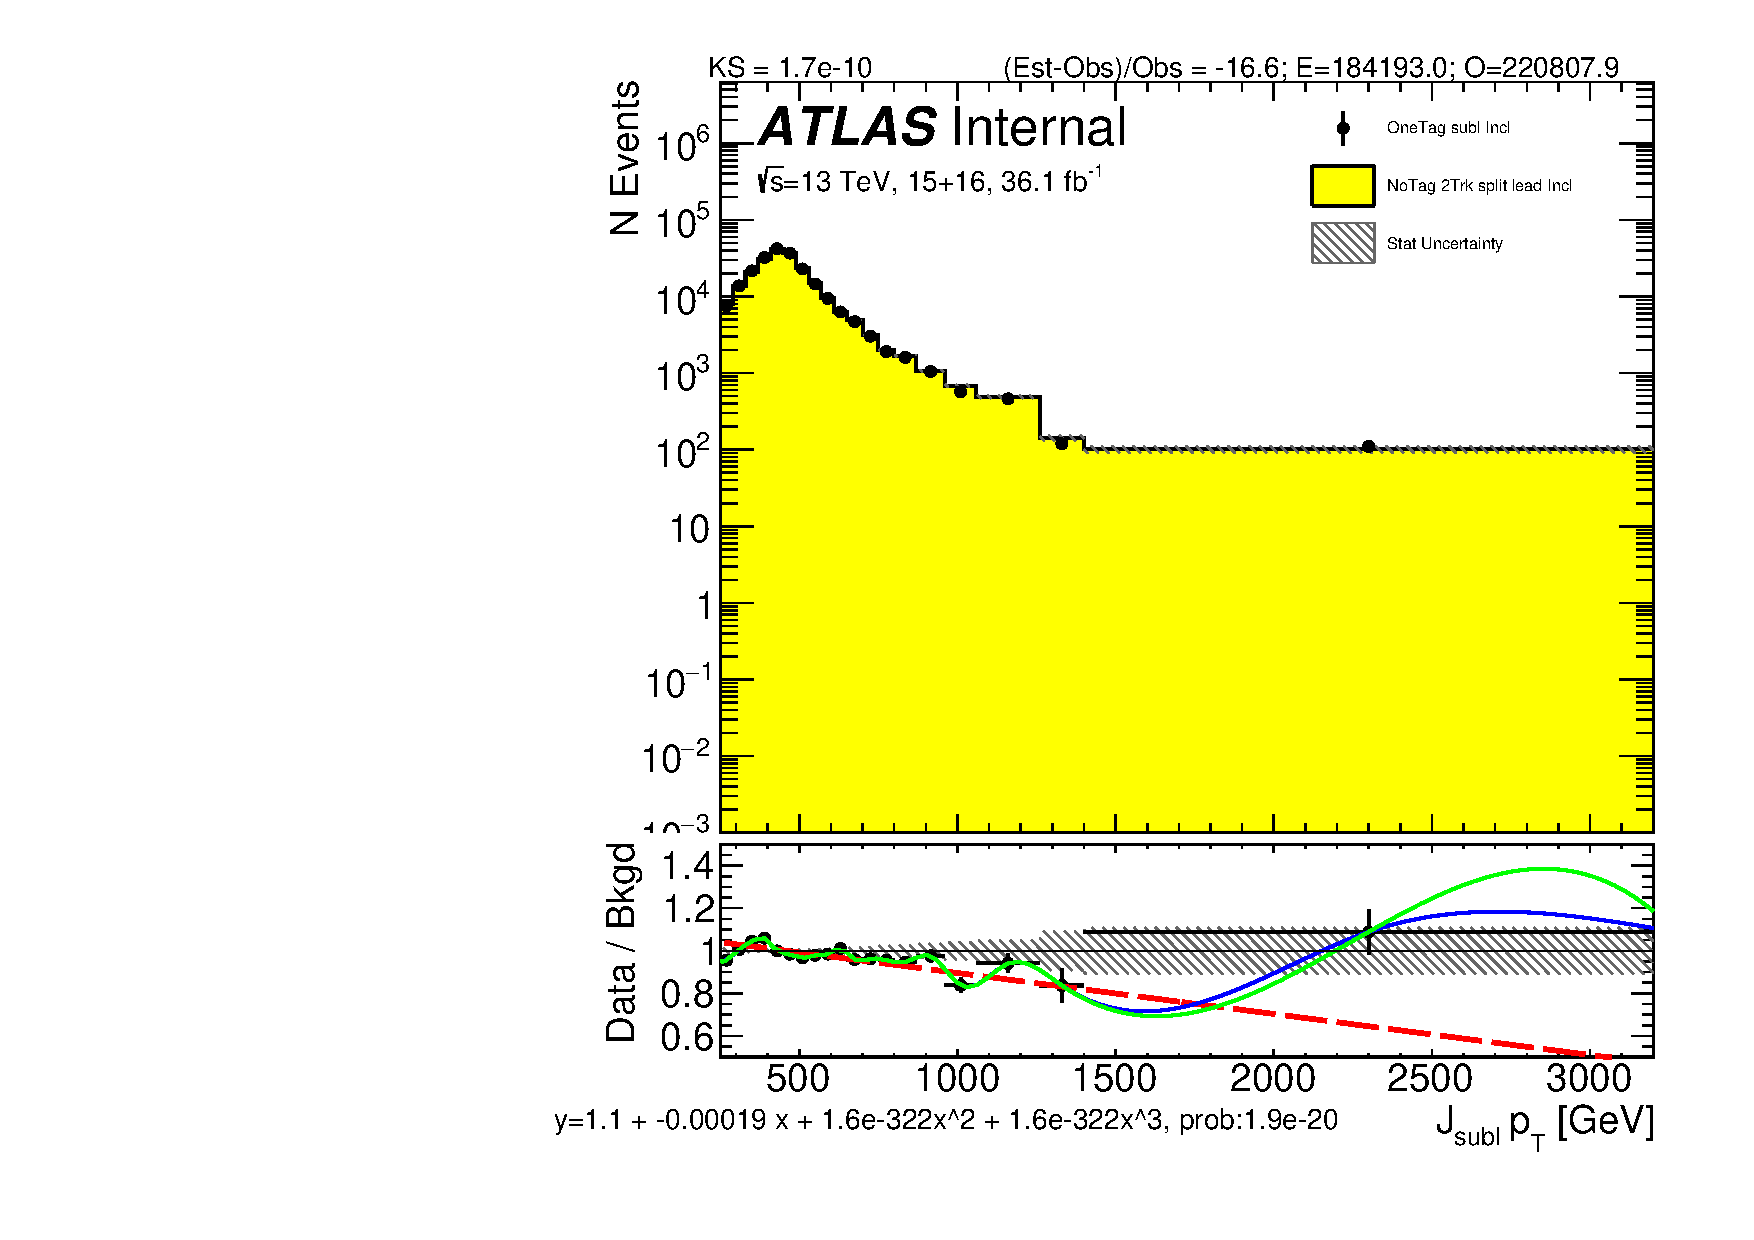
\includegraphics[width=0.25\textwidth,angle=-90]{figures/boosted/Reweight/Fits/Moriond_NoTag_2Trk_split_lead_Incl_sublHCand_Pt_m_1.pdf}
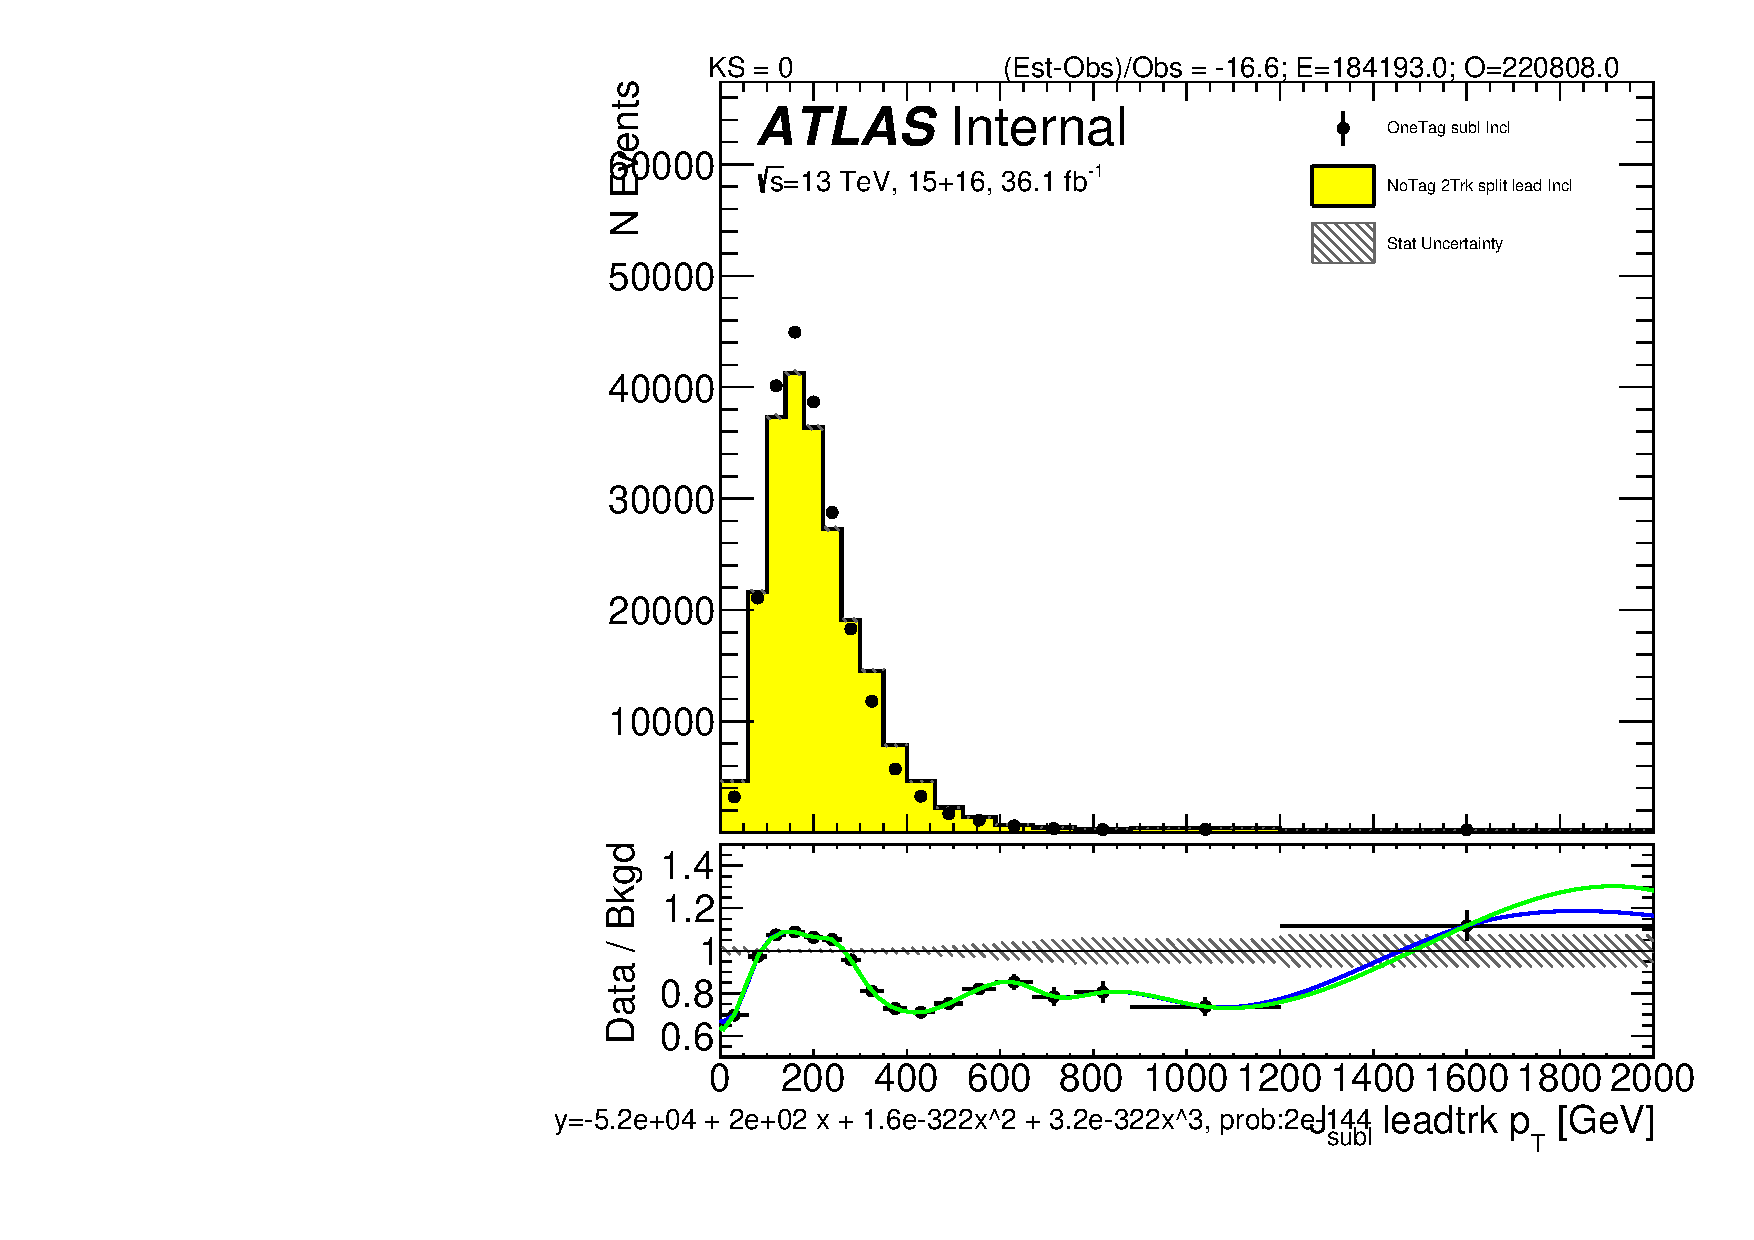
\includegraphics[width=0.25\textwidth,angle=-90]{figures/boosted/Reweight/Fits/Moriond_NoTag_2Trk_split_lead_Incl_sublHCand_trk0_Pt.pdf}
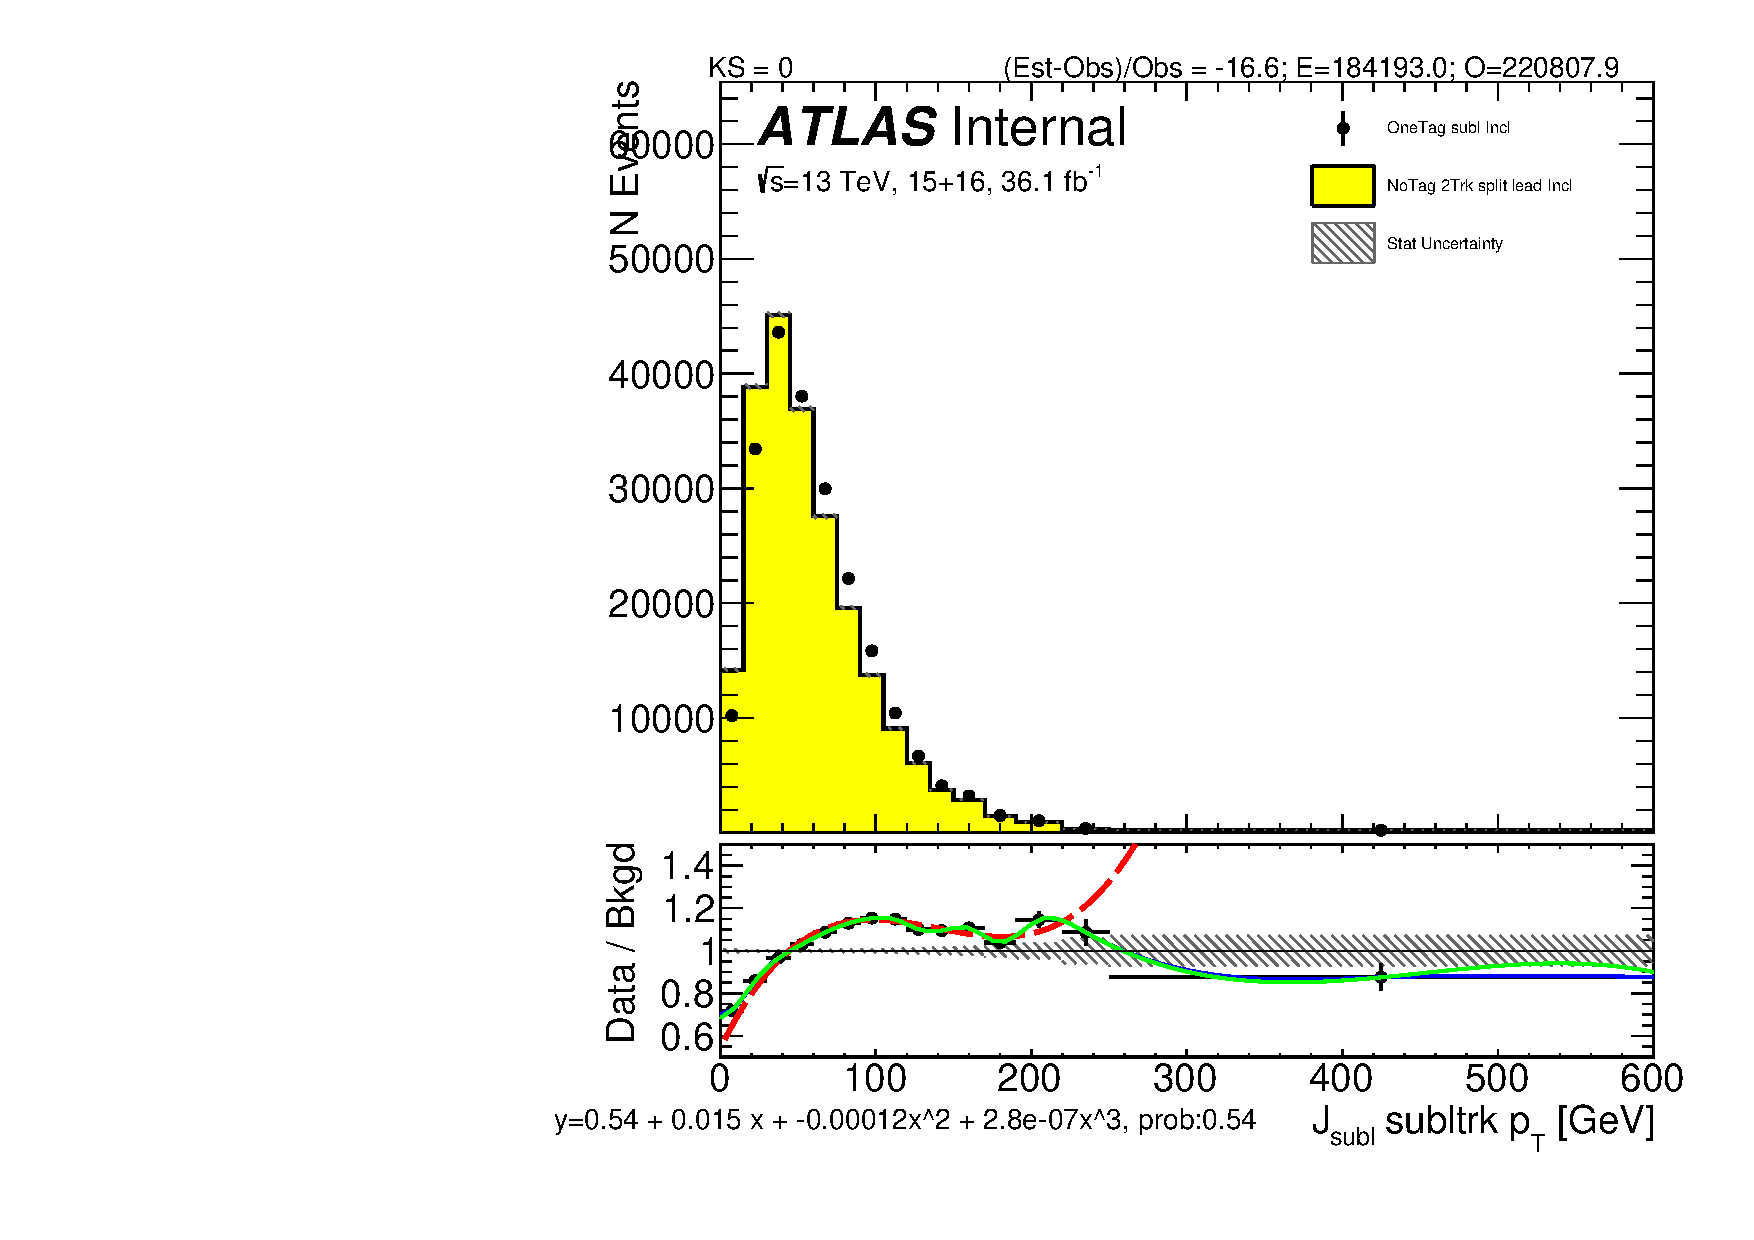
\includegraphics[width=0.25\textwidth,angle=-90]{figures/boosted/Reweight/Fits/Moriond_NoTag_2Trk_split_lead_Incl_sublHCand_trk1_Pt.pdf} \\
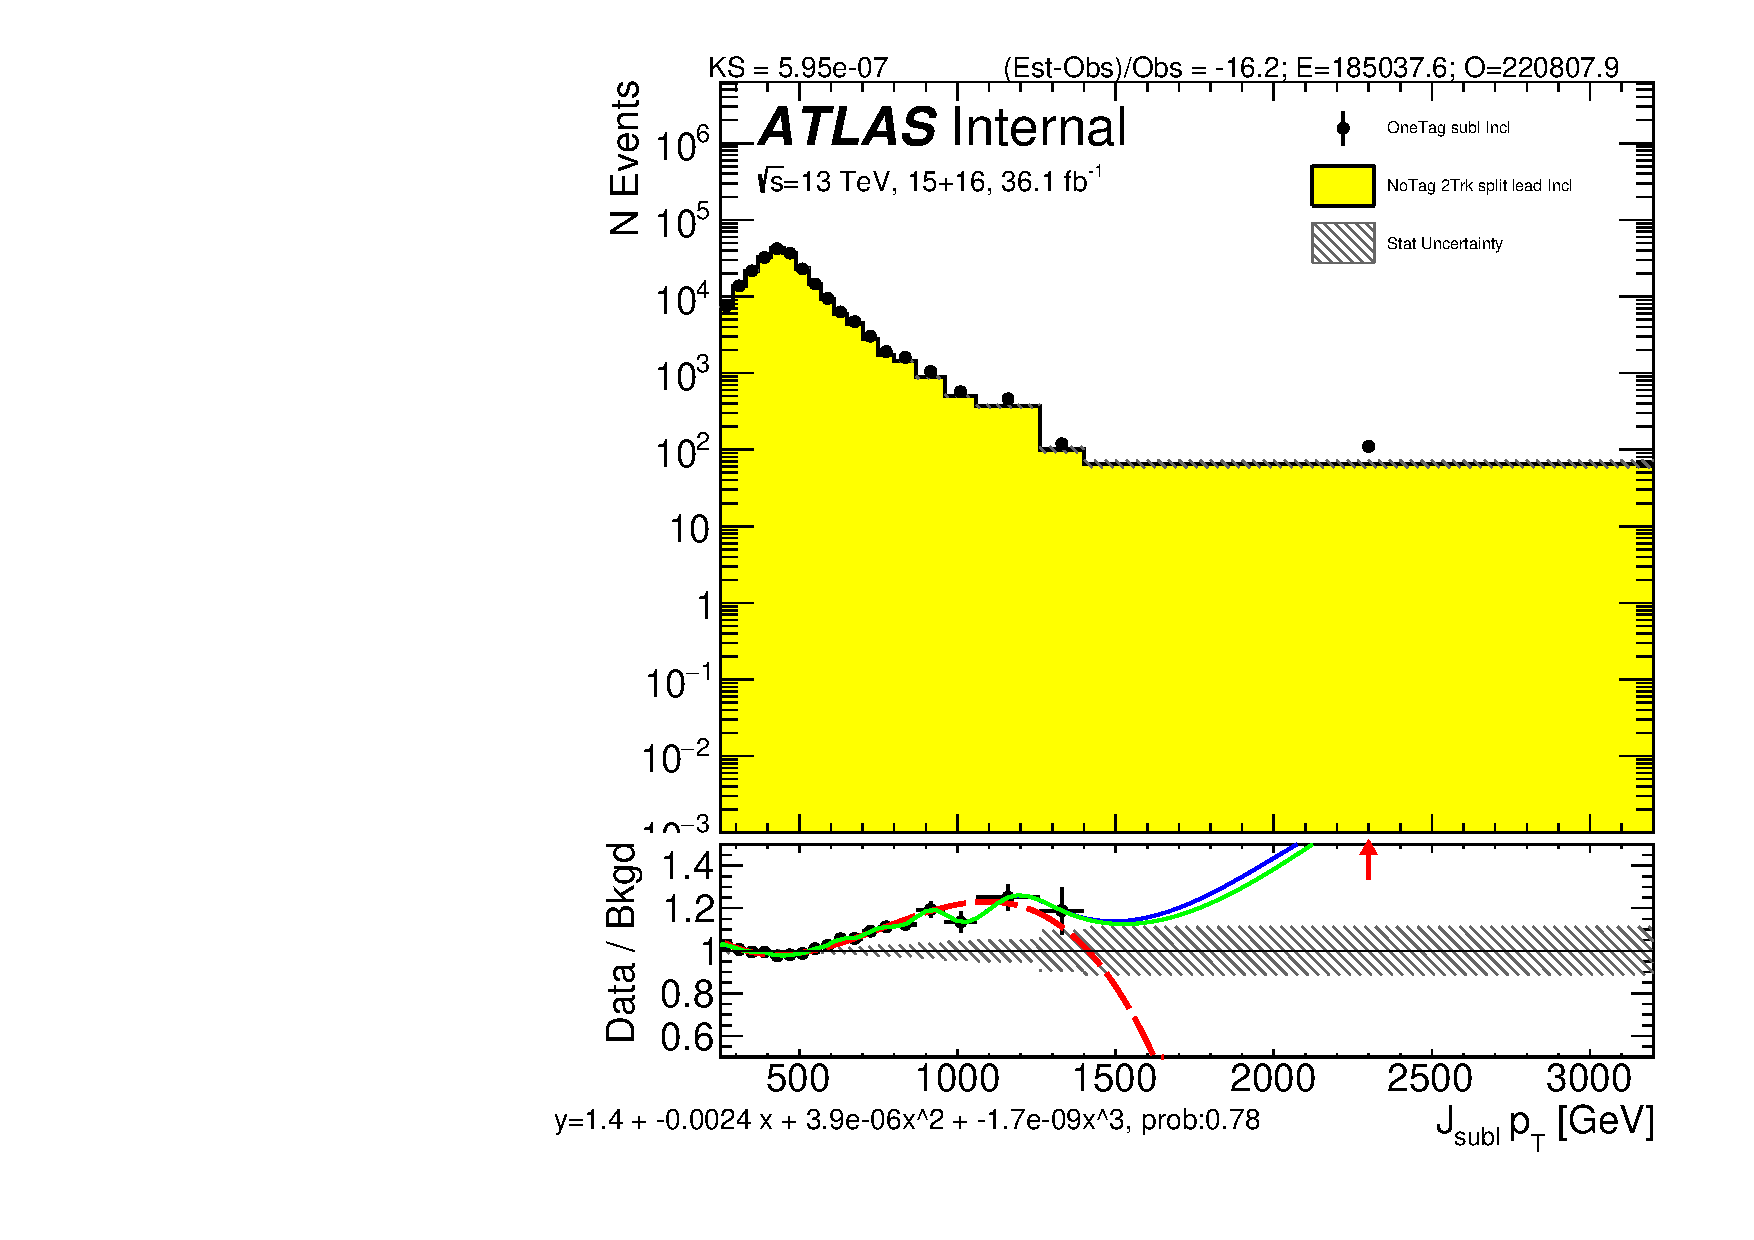
\includegraphics[width=0.25\textwidth,angle=-90]{figures/boosted/Reweight/Fits/Moriond_bkg_0_NoTag_2Trk_split_lead_Incl_sublHCand_Pt_m_1.pdf}
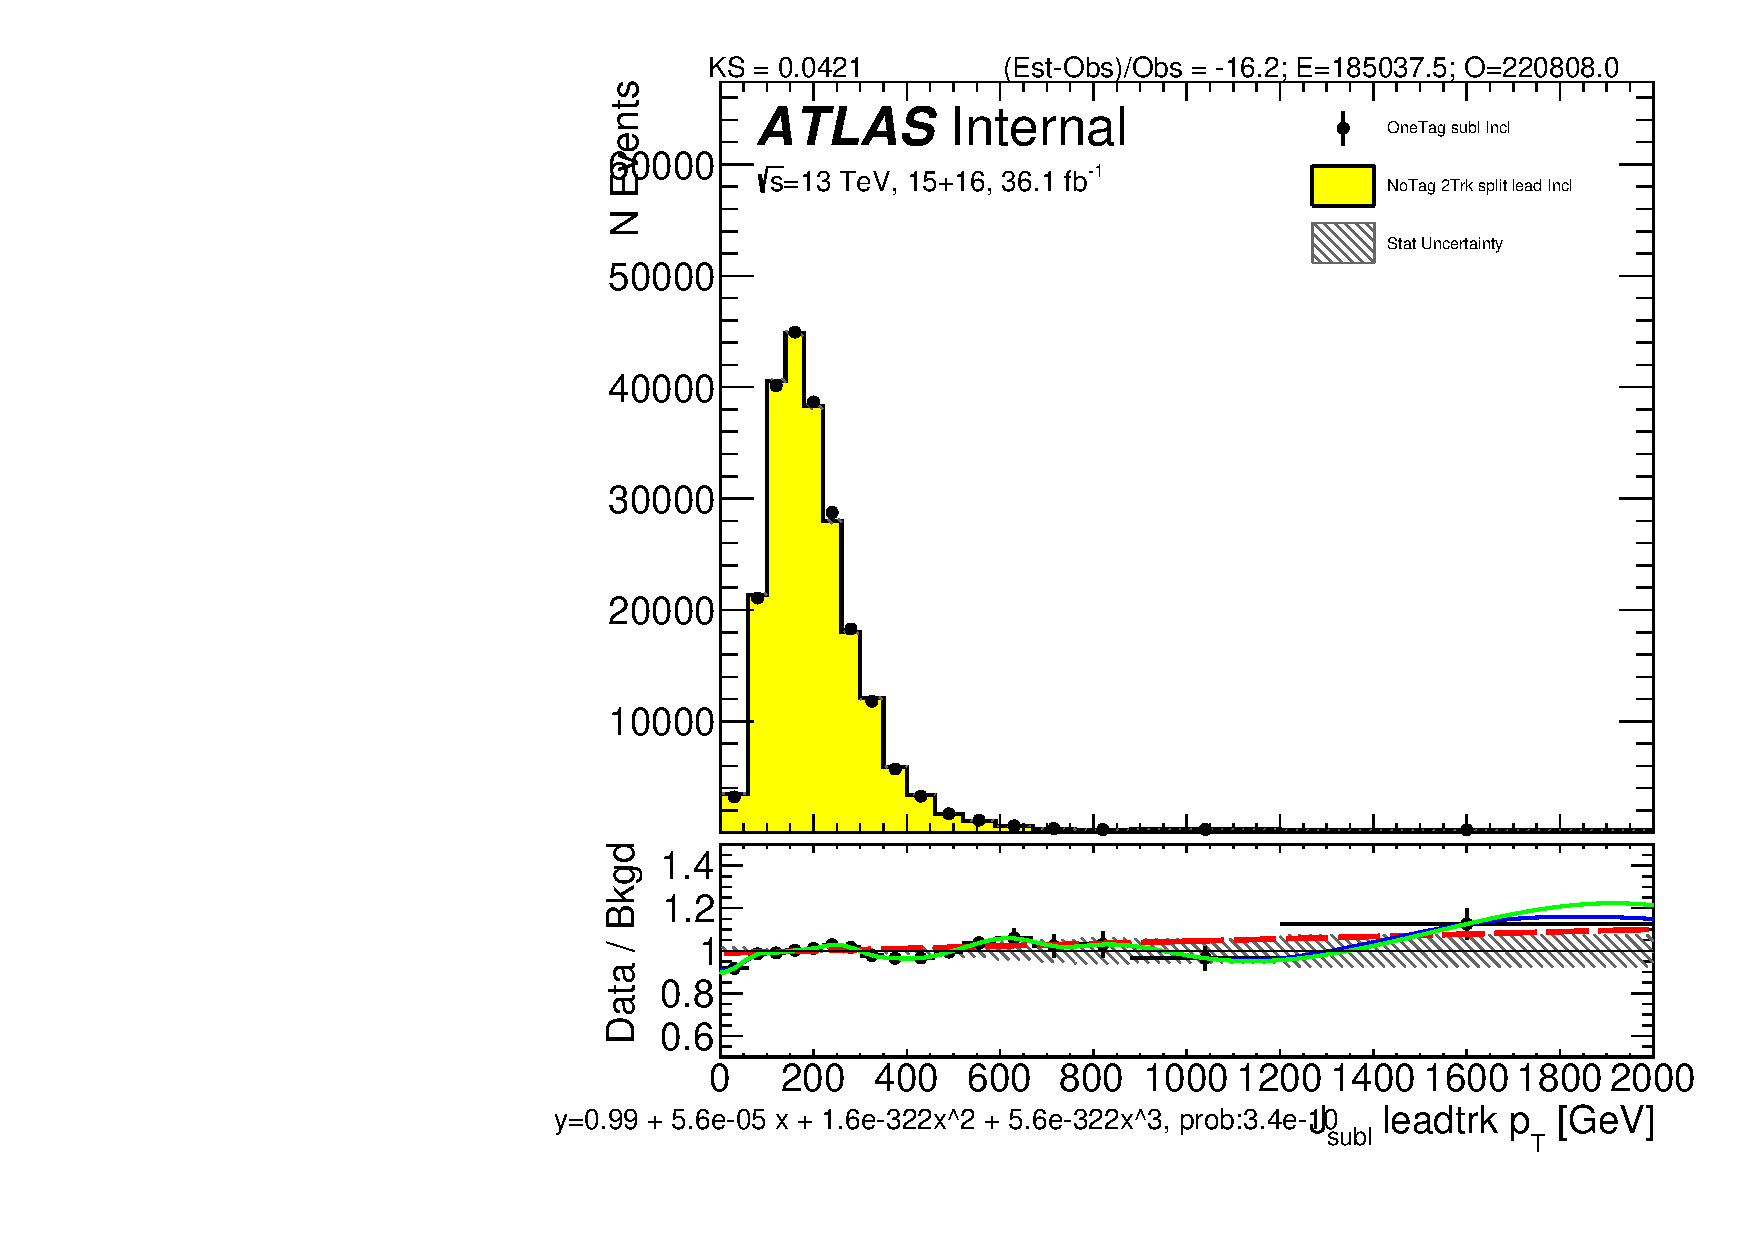
\includegraphics[width=0.25\textwidth,angle=-90]{figures/boosted/Reweight/Fits/Moriond_bkg_0_NoTag_2Trk_split_lead_Incl_sublHCand_trk0_Pt.pdf}
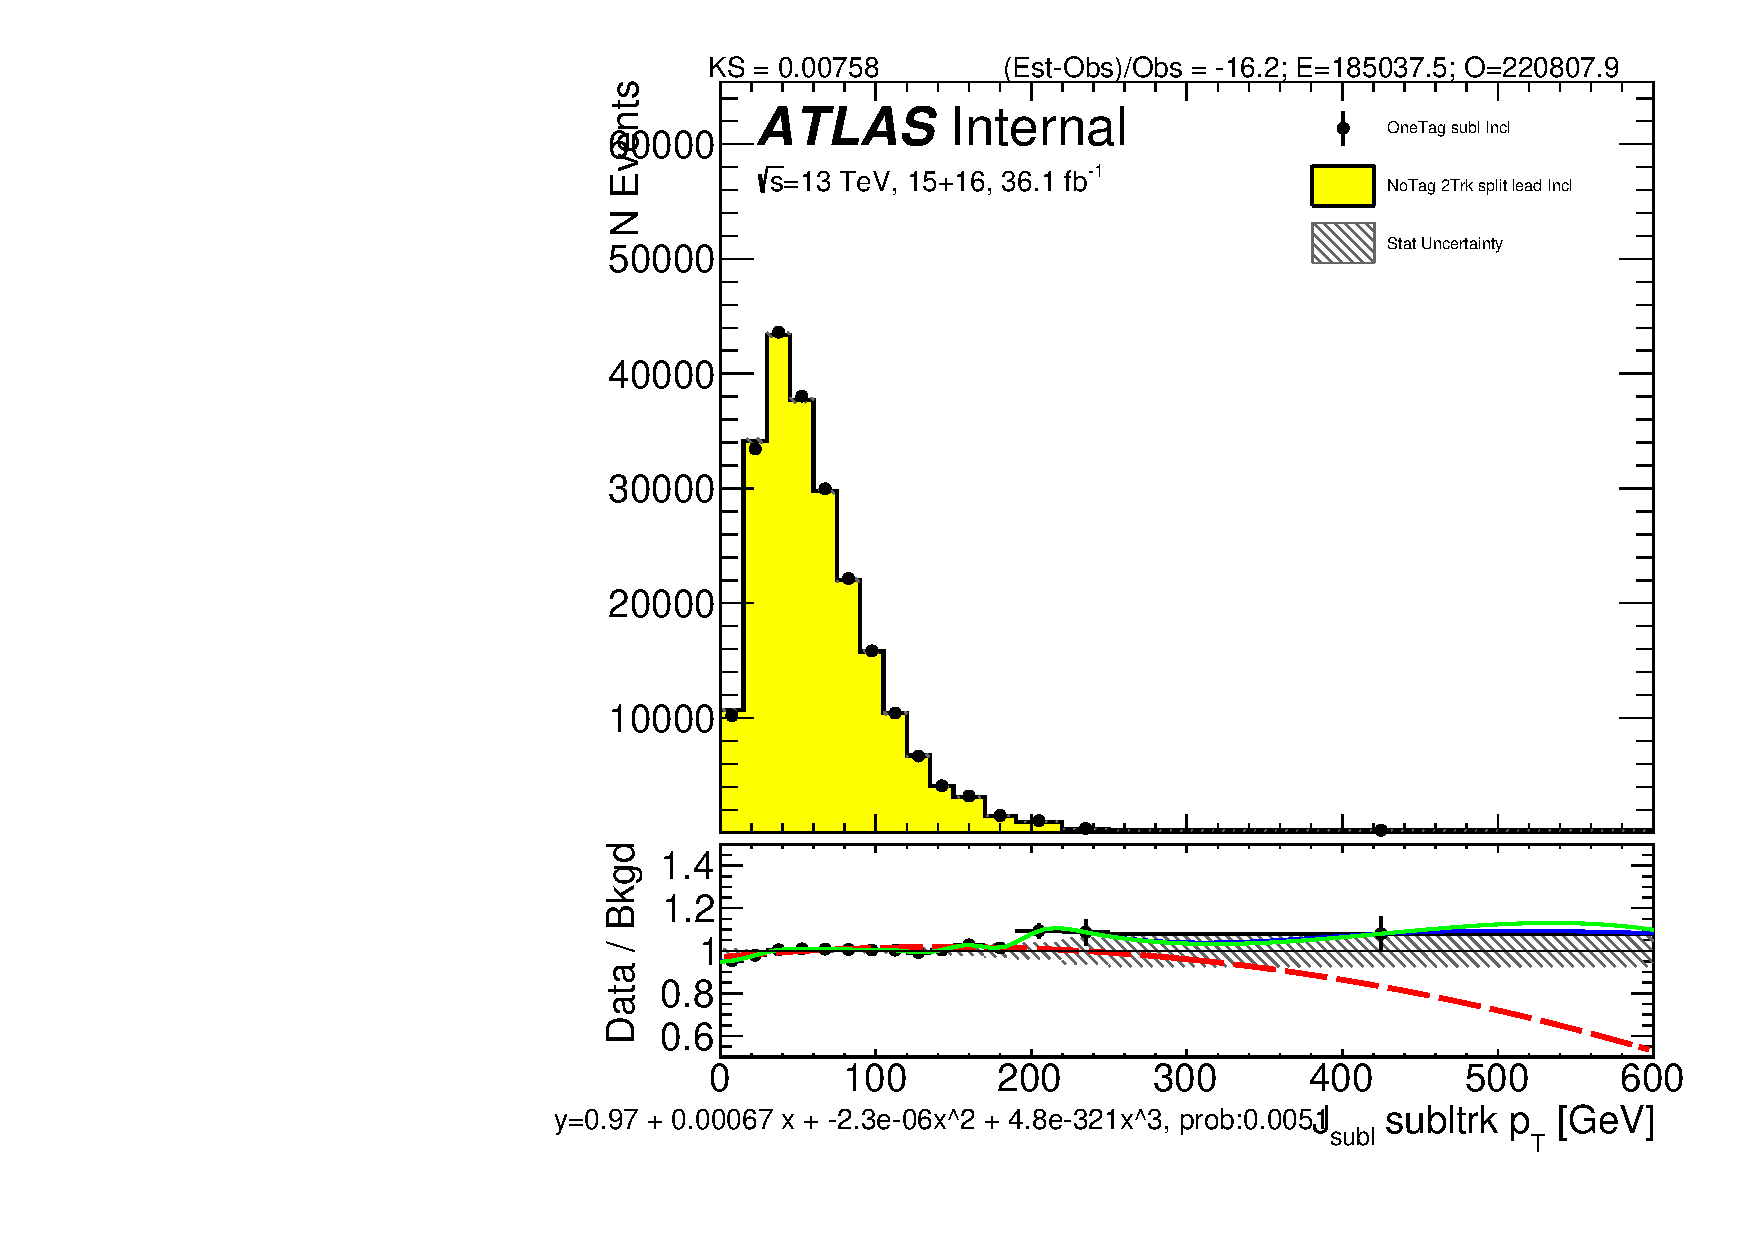
\includegraphics[width=0.25\textwidth,angle=-90]{figures/boosted/Reweight/Fits/Moriond_bkg_0_NoTag_2Trk_split_lead_Incl_sublHCand_trk1_Pt.pdf} \\
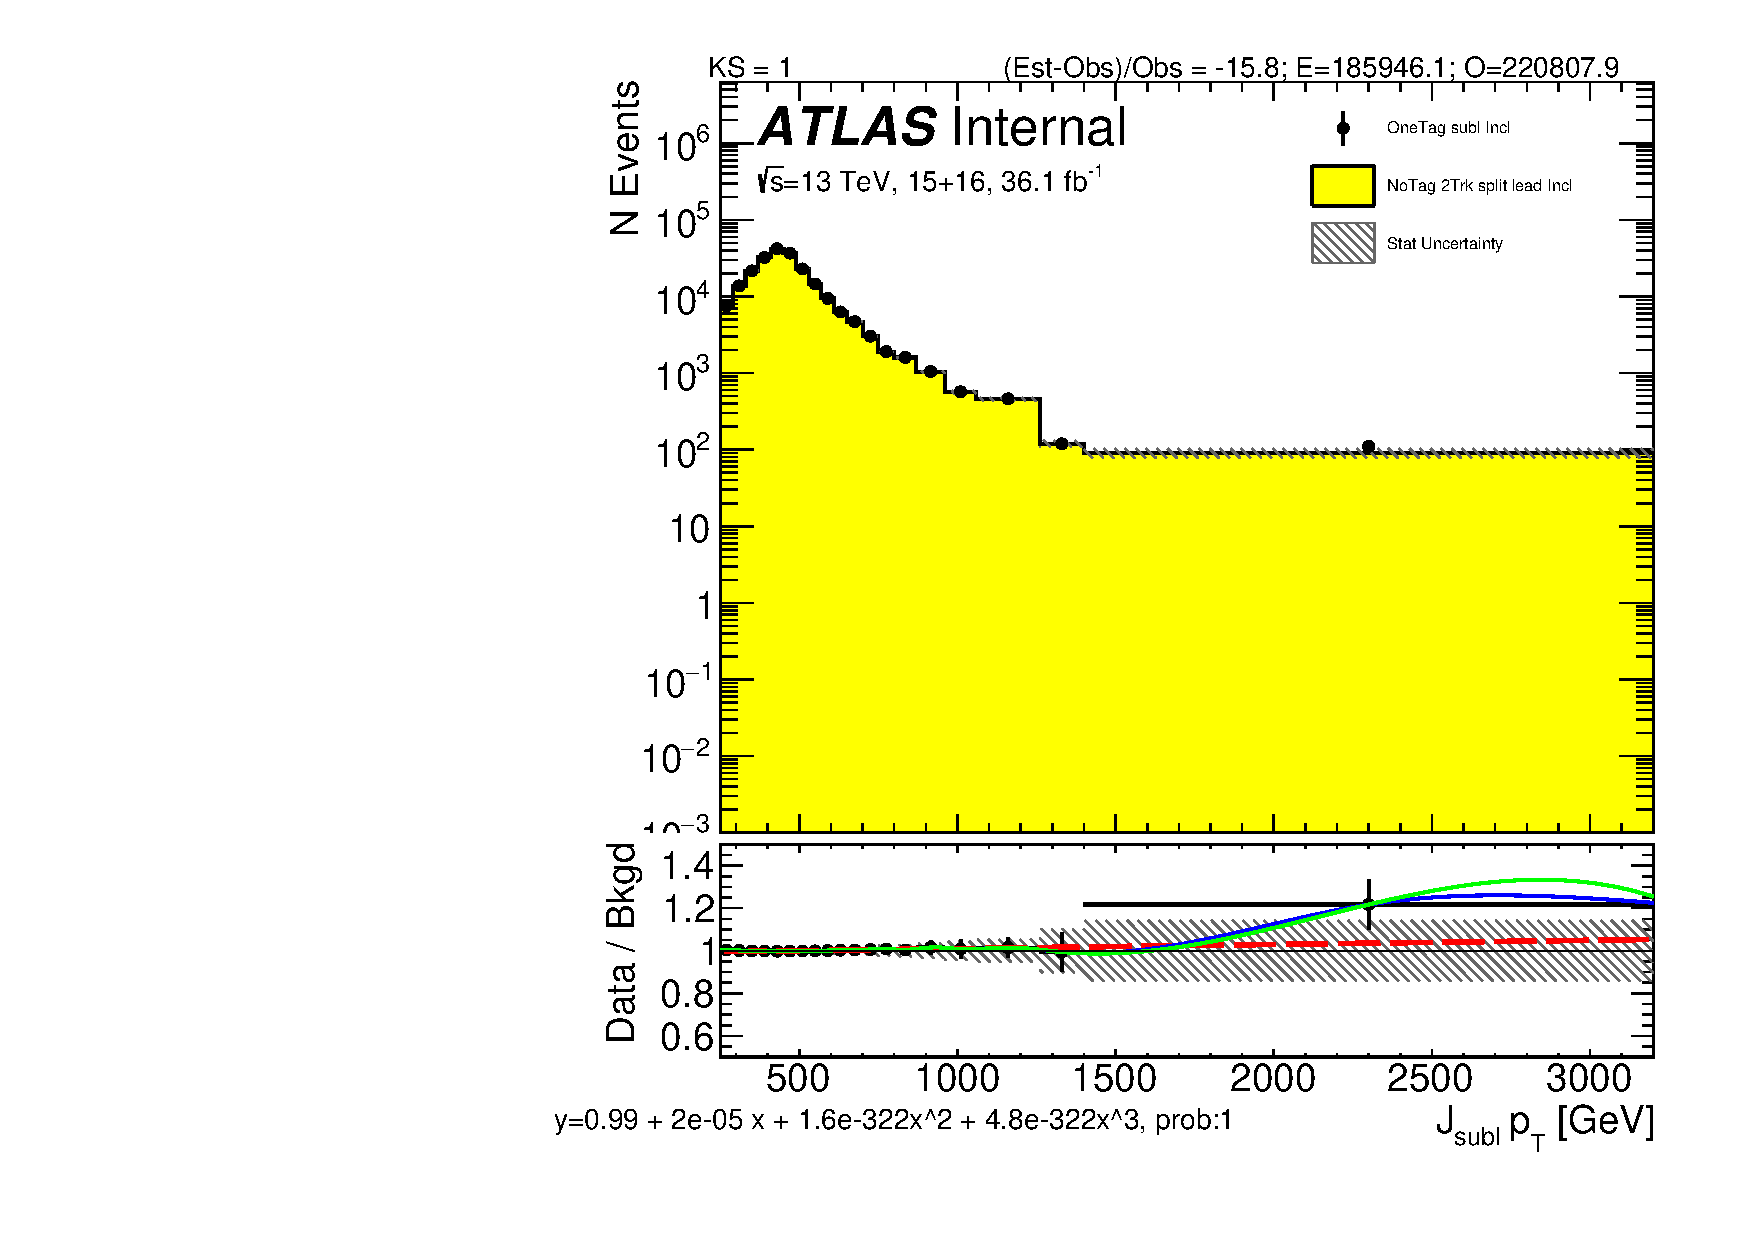
\includegraphics[width=0.25\textwidth,angle=-90]{figures/boosted/Reweight/Fits/Moriond_bkg_3_NoTag_2Trk_split_lead_Incl_sublHCand_Pt_m_1.pdf}
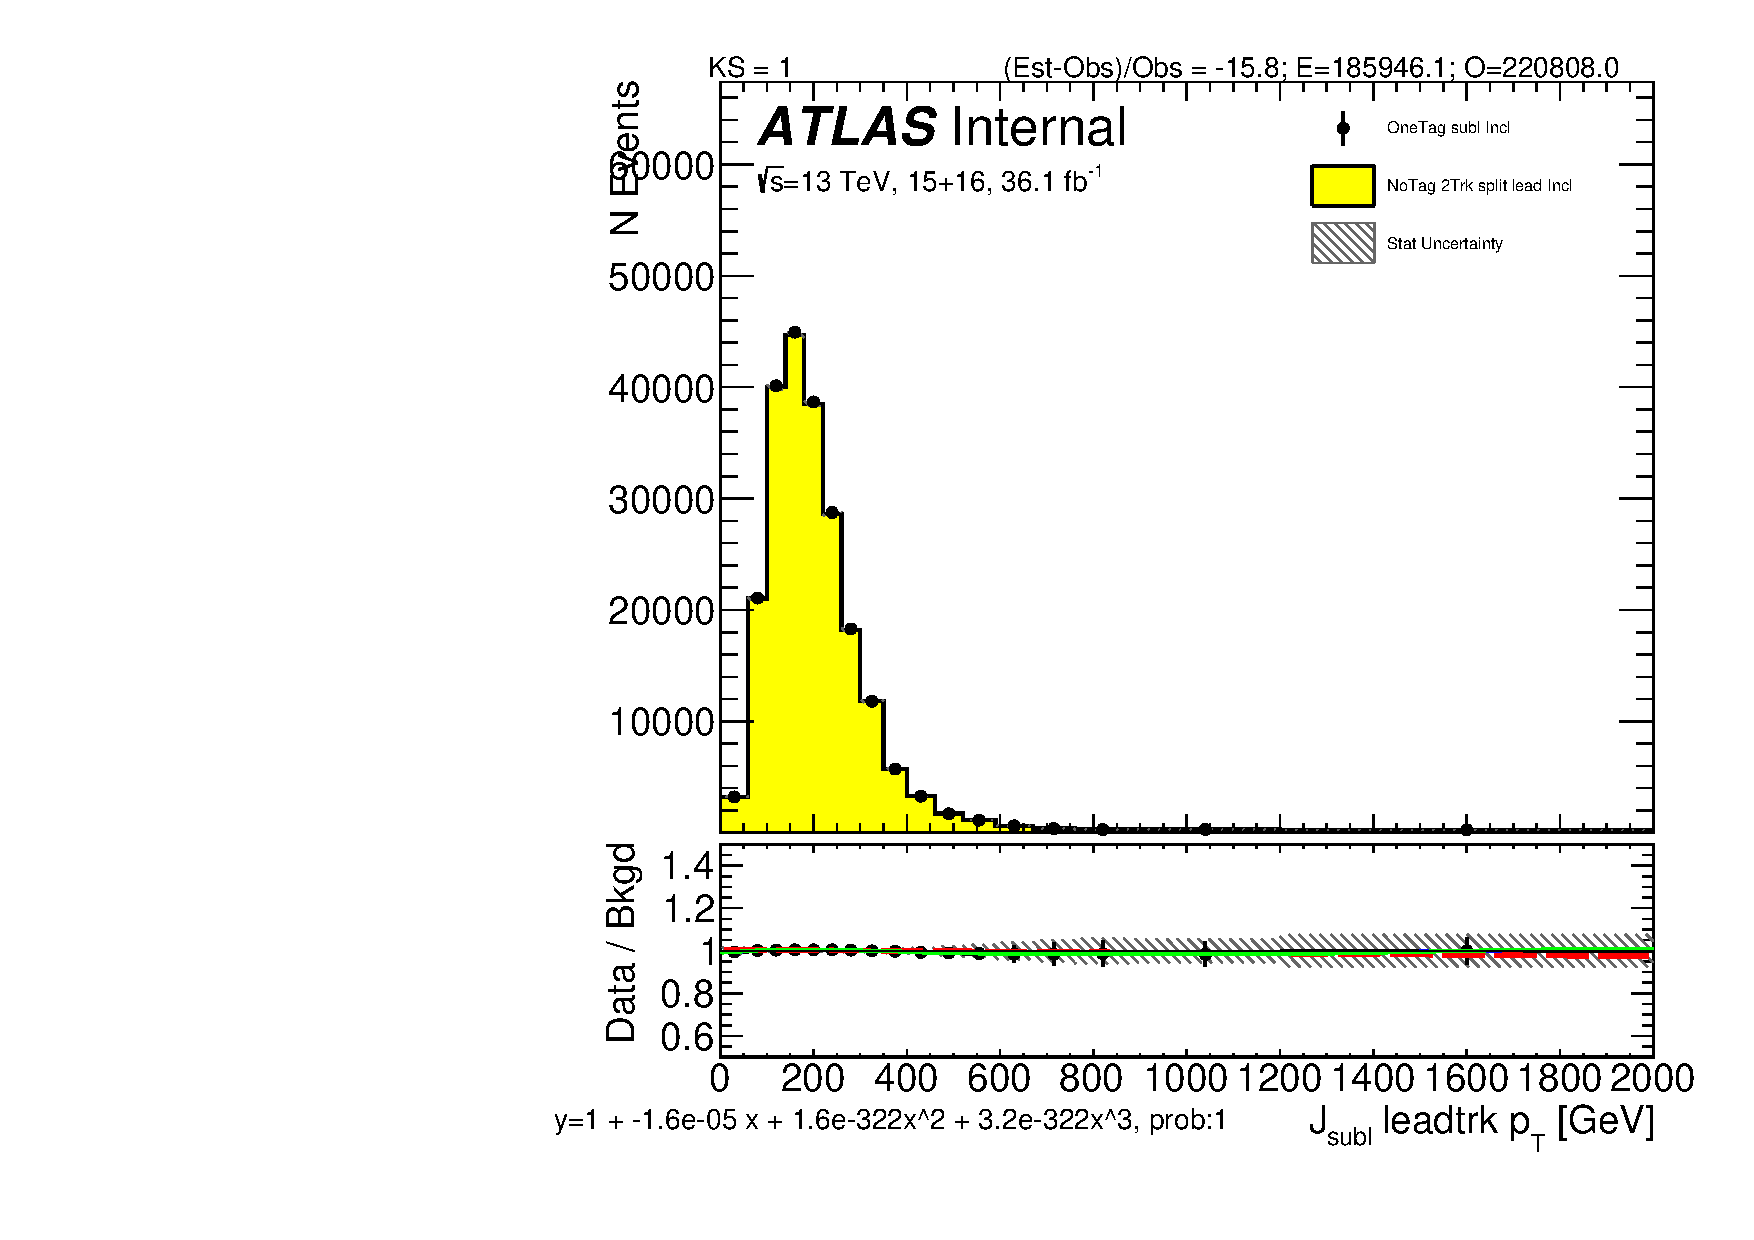
\includegraphics[width=0.25\textwidth,angle=-90]{figures/boosted/Reweight/Fits/Moriond_bkg_3_NoTag_2Trk_split_lead_Incl_sublHCand_trk0_Pt.pdf}
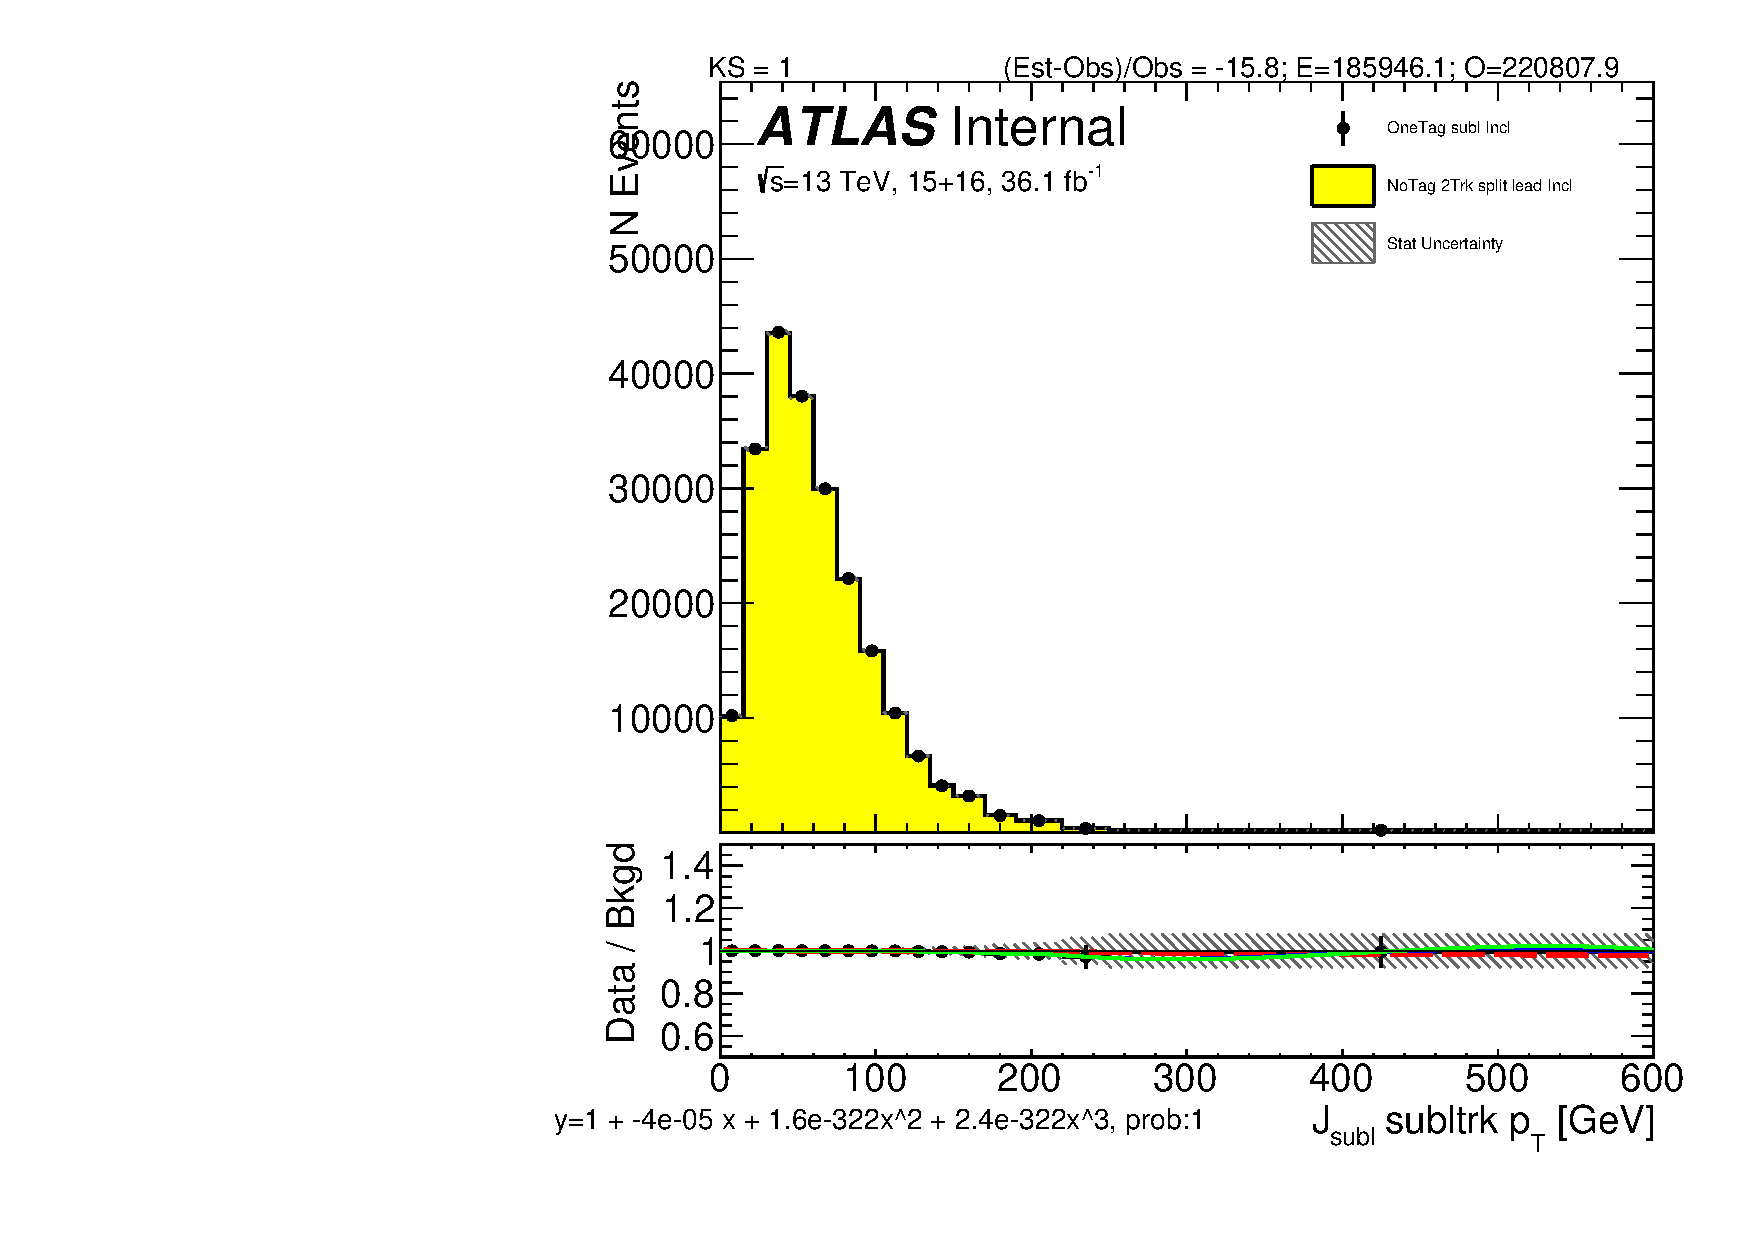
\includegraphics[width=0.25\textwidth,angle=-90]{figures/boosted/Reweight/Fits/Moriond_bkg_3_NoTag_2Trk_split_lead_Incl_sublHCand_trk1_Pt.pdf} \\
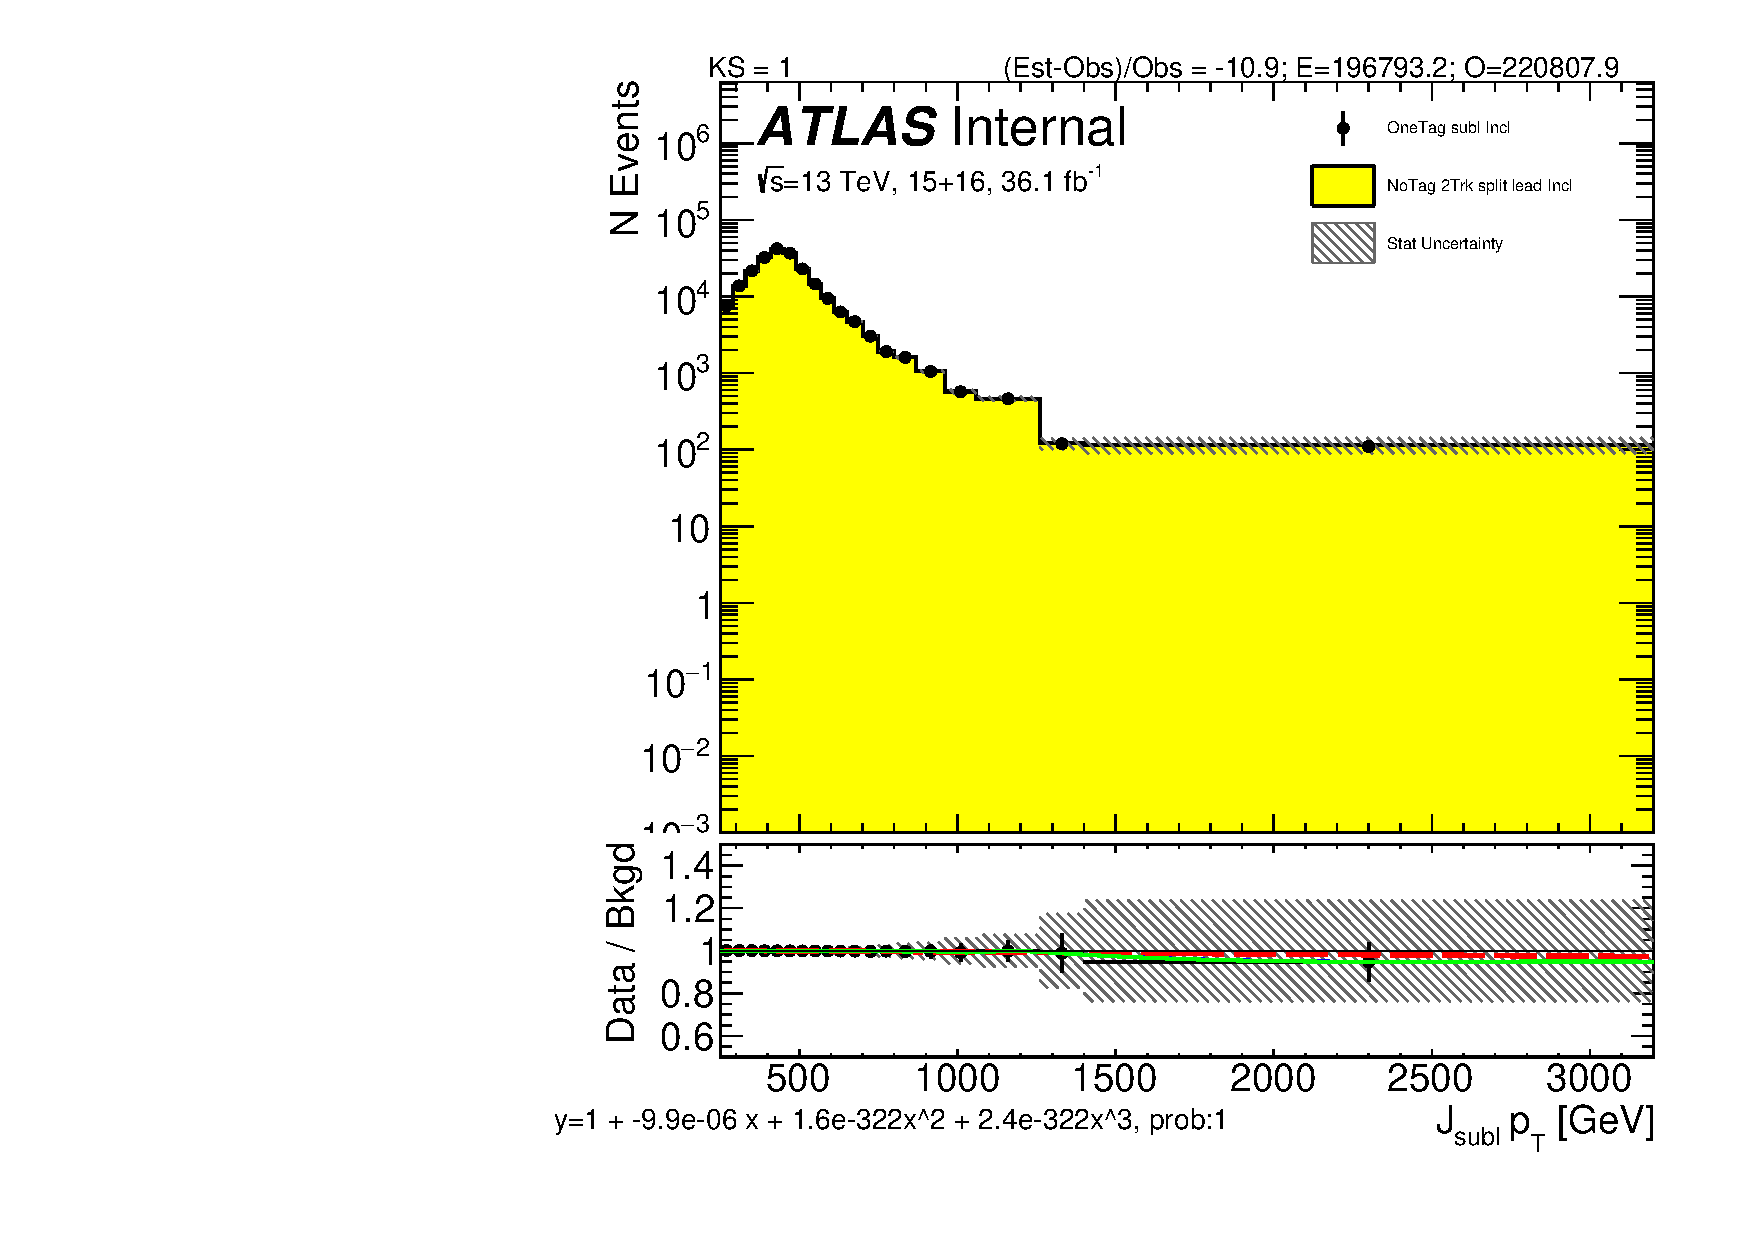
\includegraphics[width=0.25\textwidth,angle=-90]{figures/boosted/Reweight/Fits/Moriond_bkg_9_NoTag_2Trk_split_lead_Incl_sublHCand_Pt_m_1.pdf}
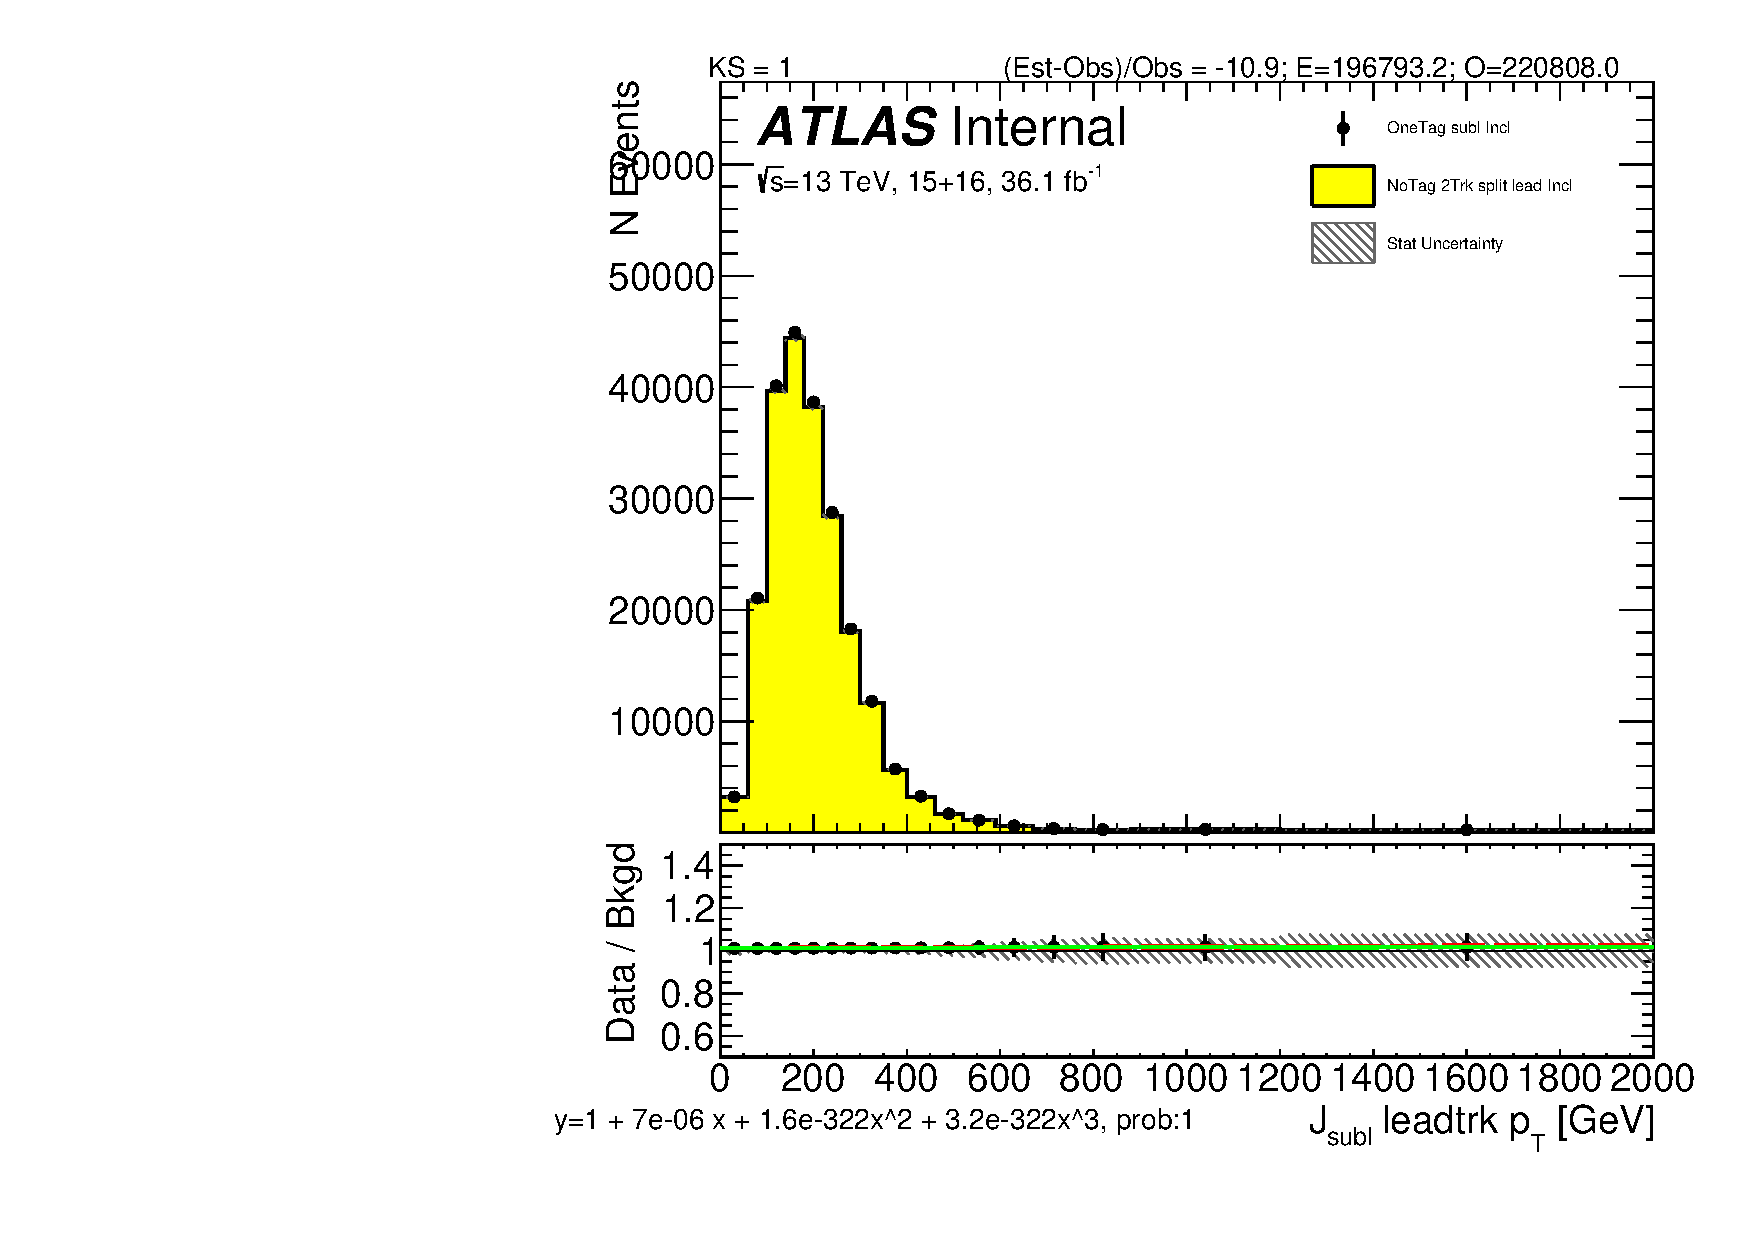
\includegraphics[width=0.25\textwidth,angle=-90]{figures/boosted/Reweight/Fits/Moriond_bkg_9_NoTag_2Trk_split_lead_Incl_sublHCand_trk0_Pt.pdf}
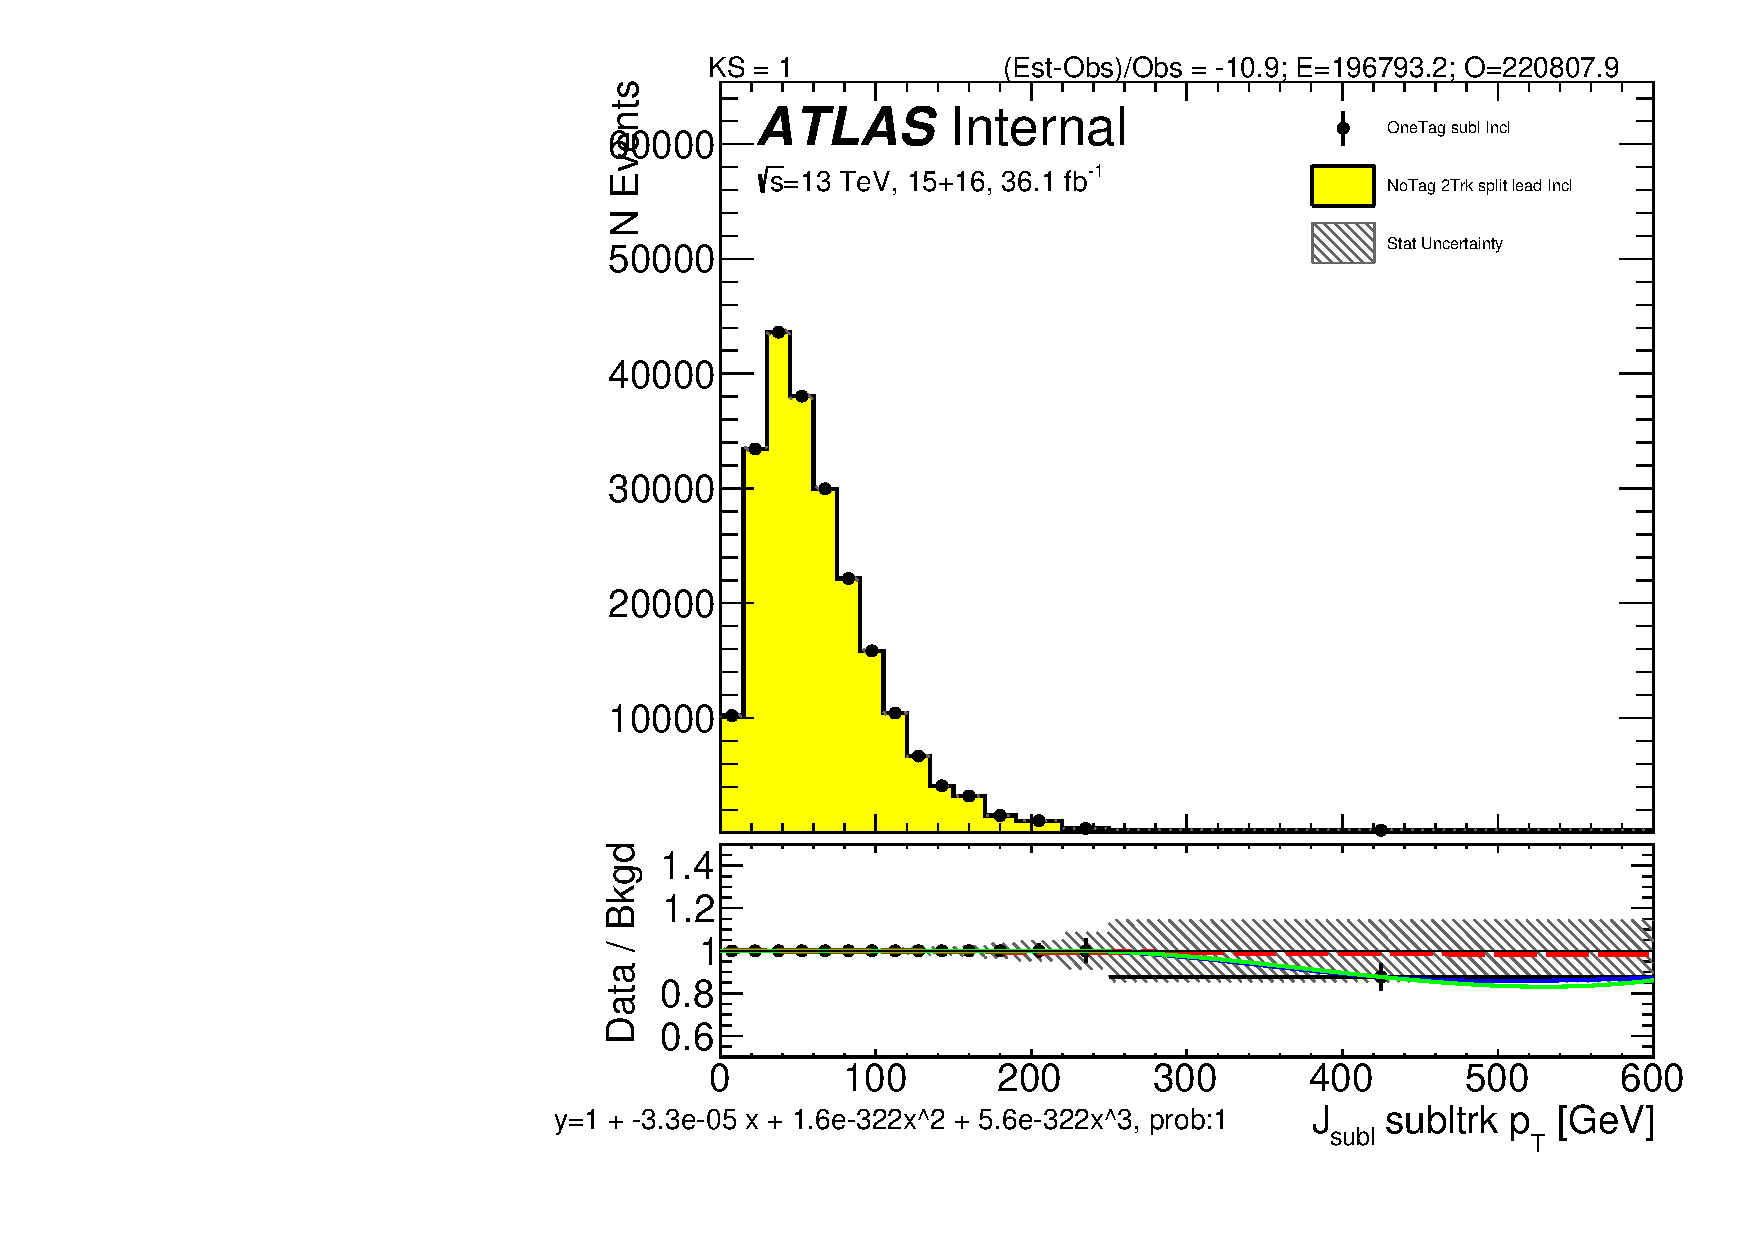
\includegraphics[width=0.25\textwidth,angle=-90]{figures/boosted/Reweight/Fits/Moriond_bkg_9_NoTag_2Trk_split_lead_Incl_sublHCand_trk1_Pt.pdf} \\
\caption{For $2bs$ background estimate: the fits to the ratio of the data in the $1b$ category, of the subleading Higgs candidate $1b$-tagged events' subleading Higgs candidate distributions(black point), over the leading Higgs candidate $1b$-tagged events' subleading Higgs candidate distributions(yellow). Distributions and fits to the estimated QCD background for large-\R jet $p_{T}$ (left), the large-\R jet's leading track jet $p_T$ (middle), and large-\R jet's subleading track jet $p_T$ (right) are shown.  Figures are before reweighting (top row), after the first iteration(second row), after the fourth iteration(third row), and after the last iteration (bottom row). The green line is the spline fit; the red line is a polynomial fit; the blue line is the spline interpolation.}
\label{fig:rw-2bs-lead}
\end{center}
\end{figure*}

\begin{figure*}[htbp!]
\begin{center}
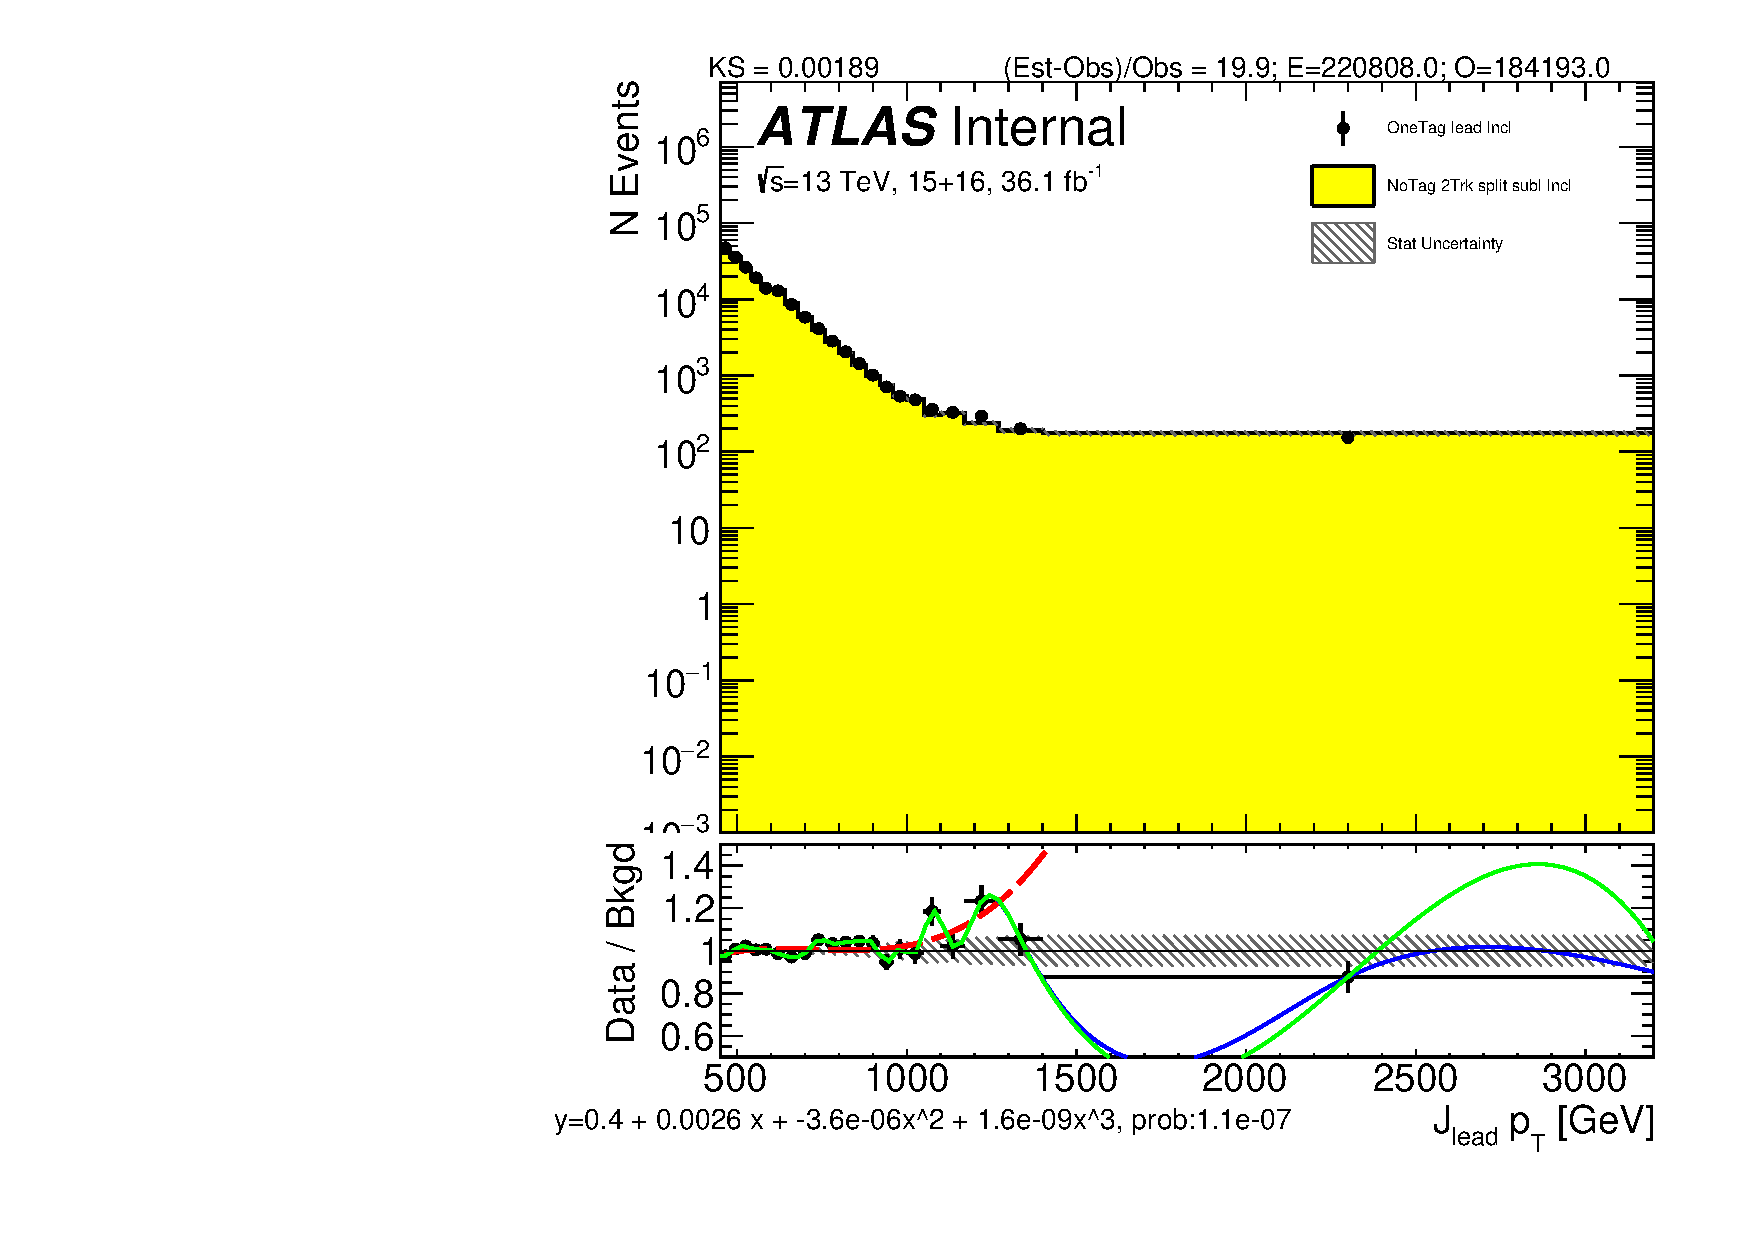
\includegraphics[width=0.25\textwidth,angle=-90]{figures/boosted/Reweight/Fits/Moriond_NoTag_2Trk_split_subl_Incl_leadHCand_Pt_m_1.pdf}
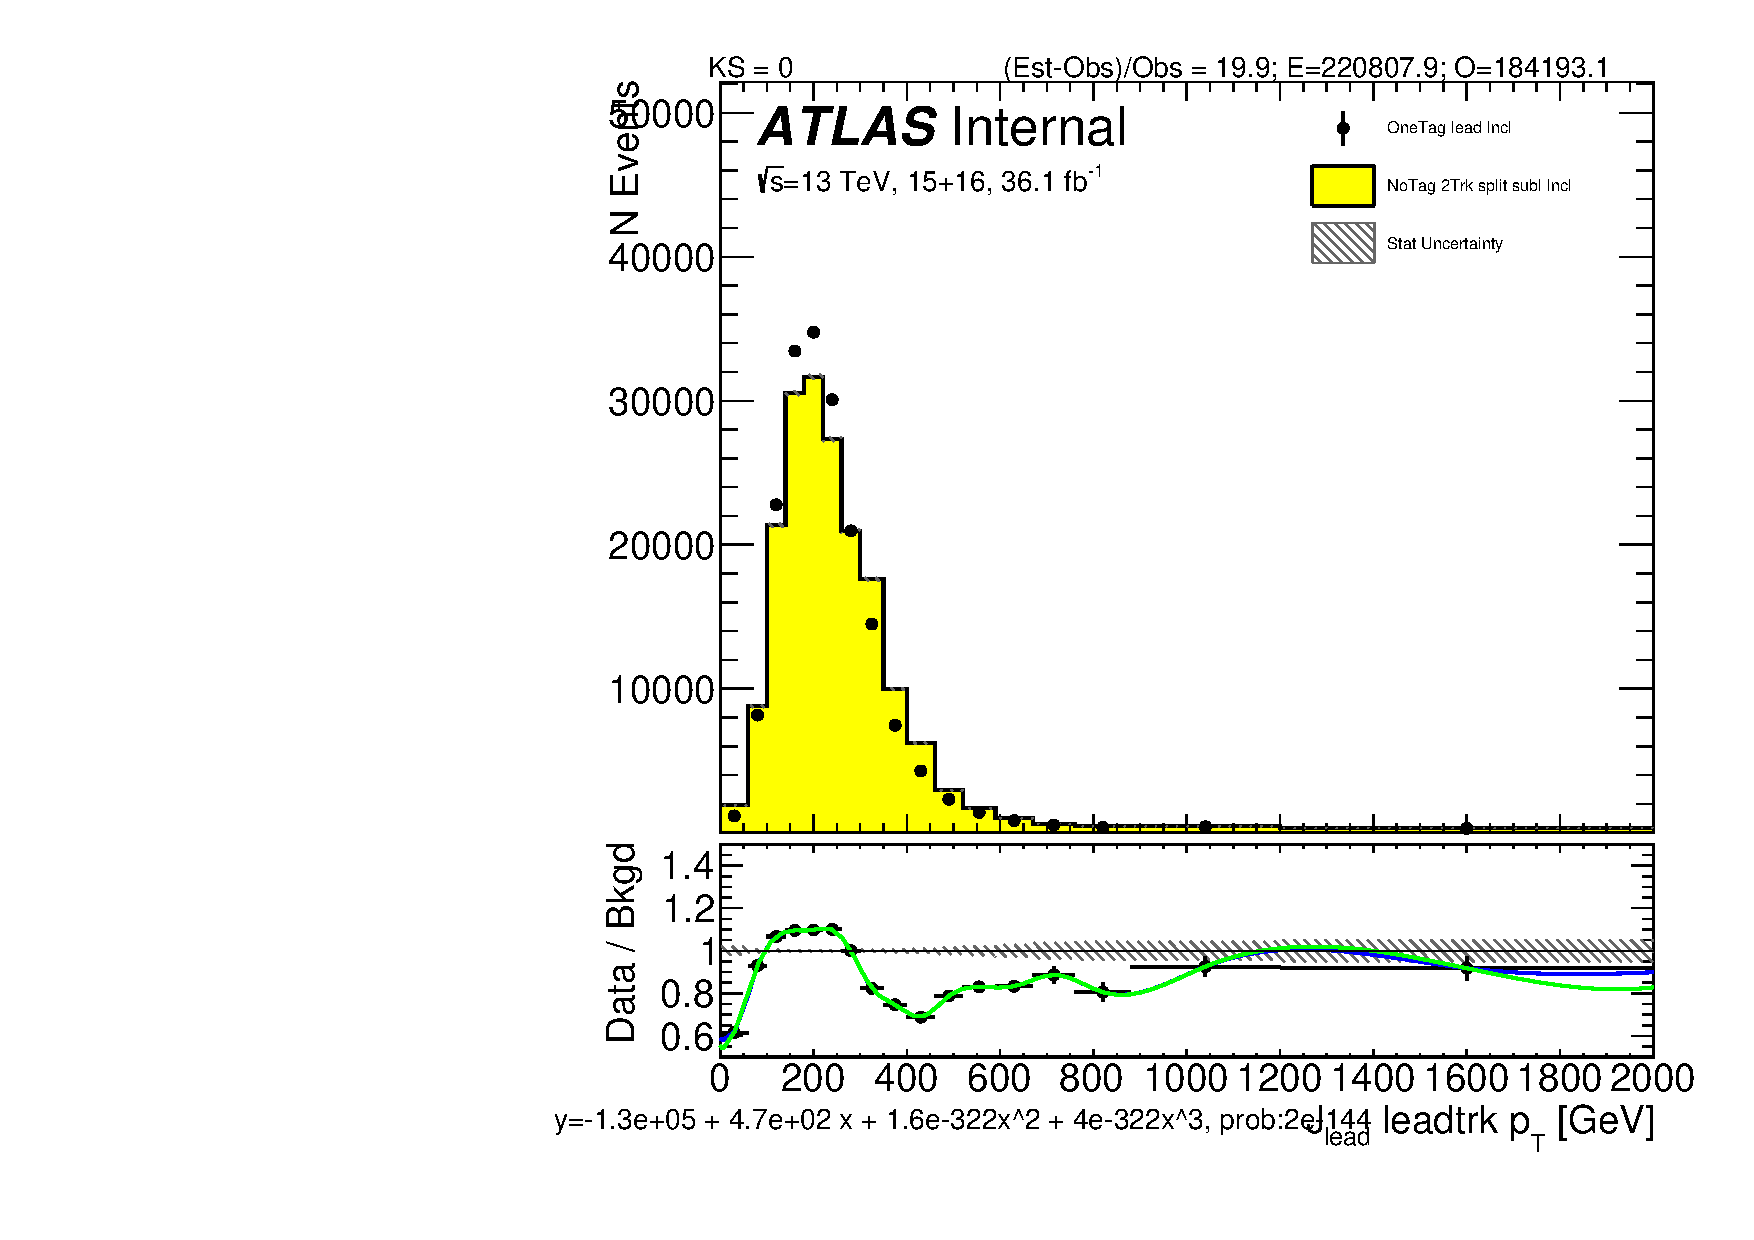
\includegraphics[width=0.25\textwidth,angle=-90]{figures/boosted/Reweight/Fits/Moriond_NoTag_2Trk_split_subl_Incl_leadHCand_trk0_Pt.pdf}
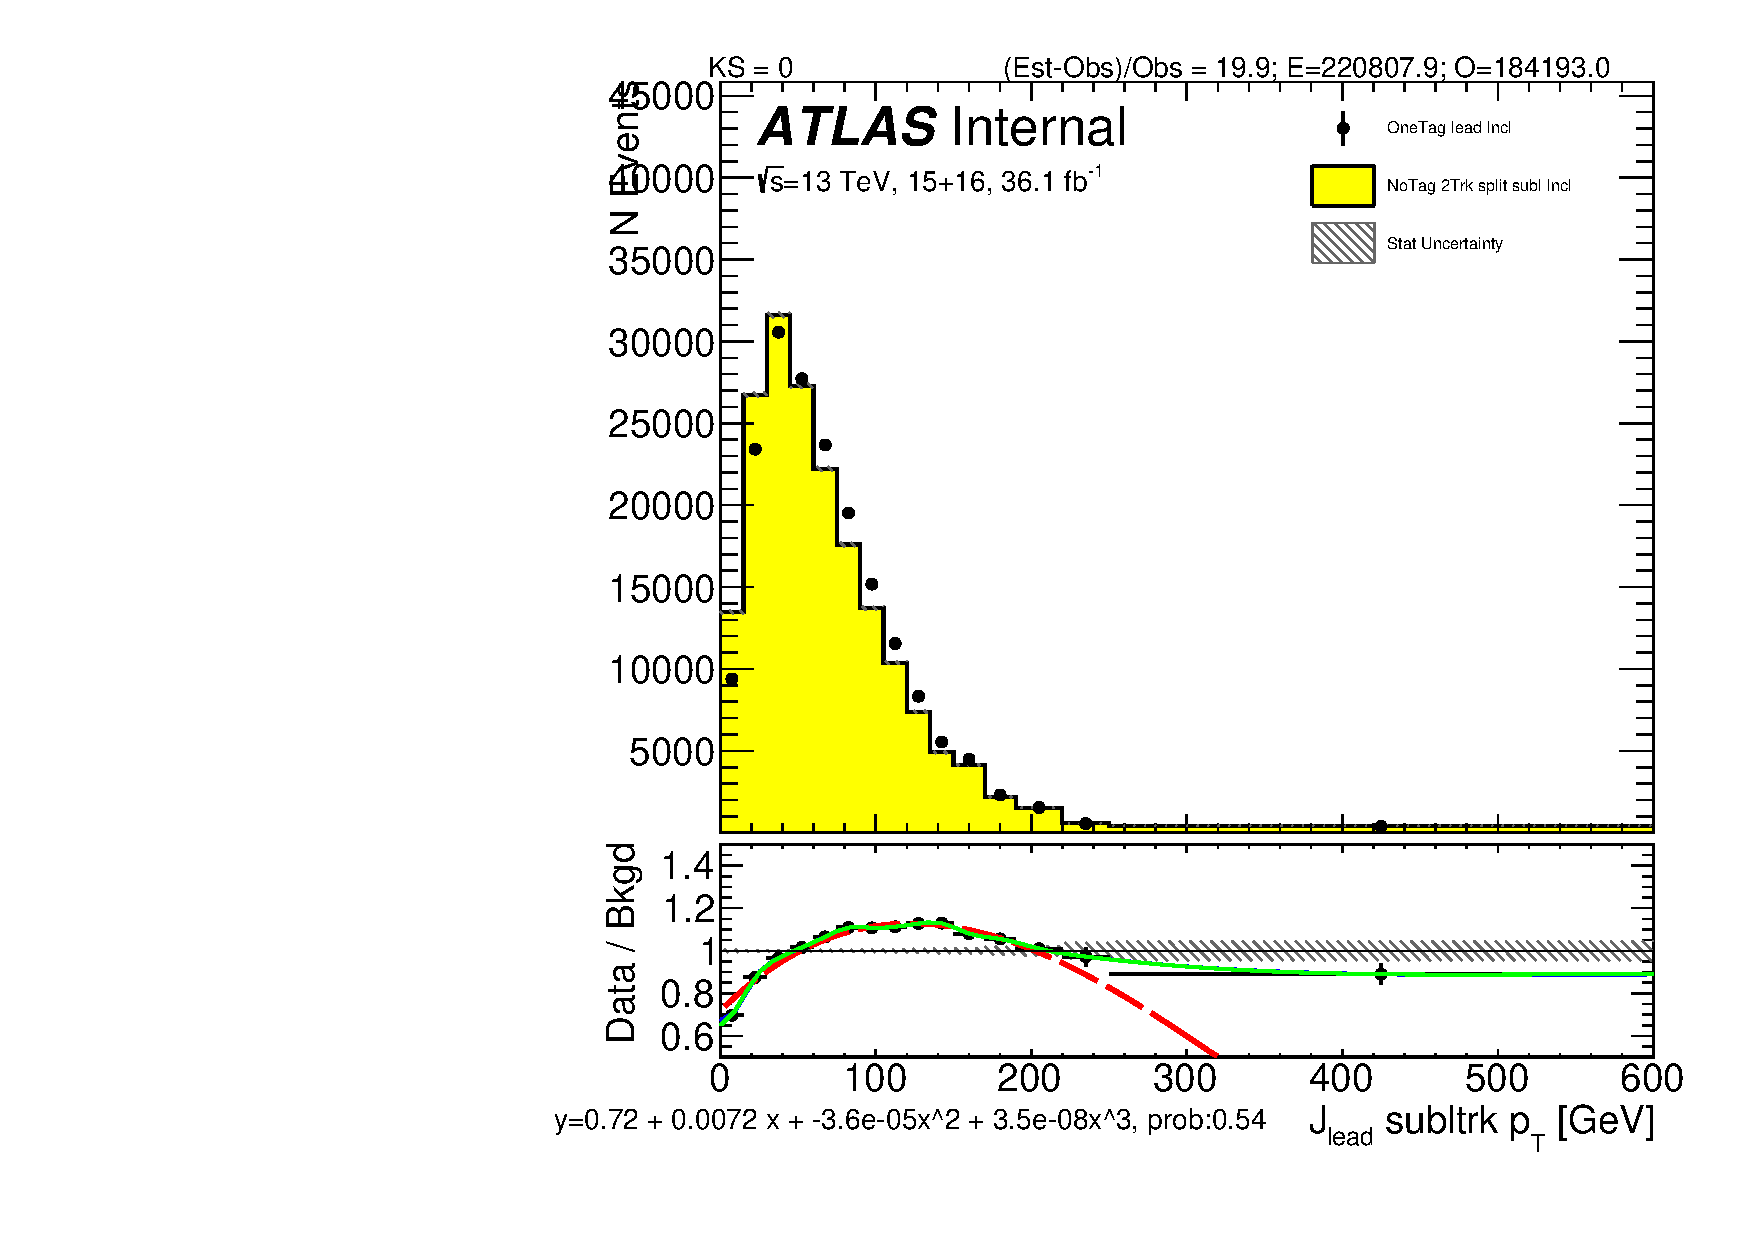
\includegraphics[width=0.25\textwidth,angle=-90]{figures/boosted/Reweight/Fits/Moriond_NoTag_2Trk_split_subl_Incl_leadHCand_trk1_Pt.pdf} \\
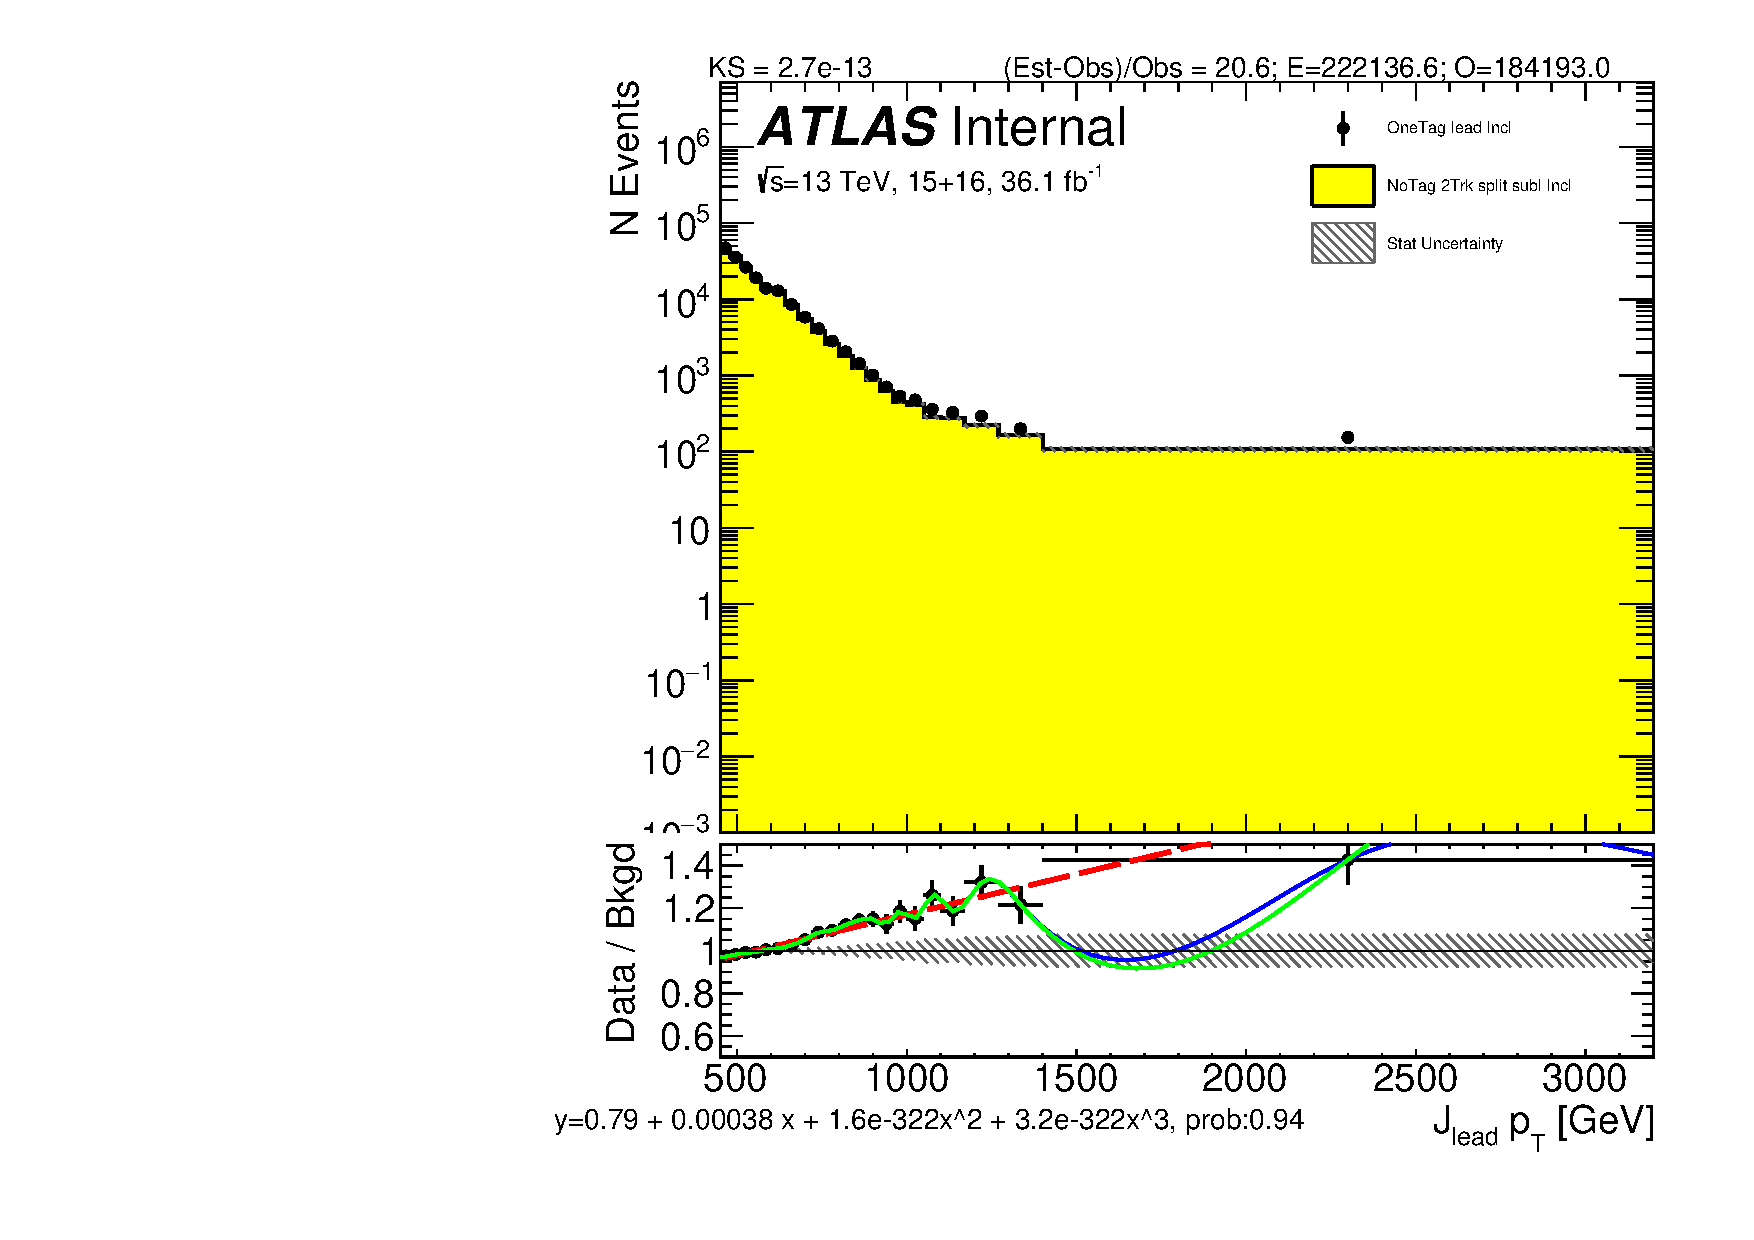
\includegraphics[width=0.25\textwidth,angle=-90]{figures/boosted/Reweight/Fits/Moriond_bkg_0_NoTag_2Trk_split_subl_Incl_leadHCand_Pt_m_1.pdf}
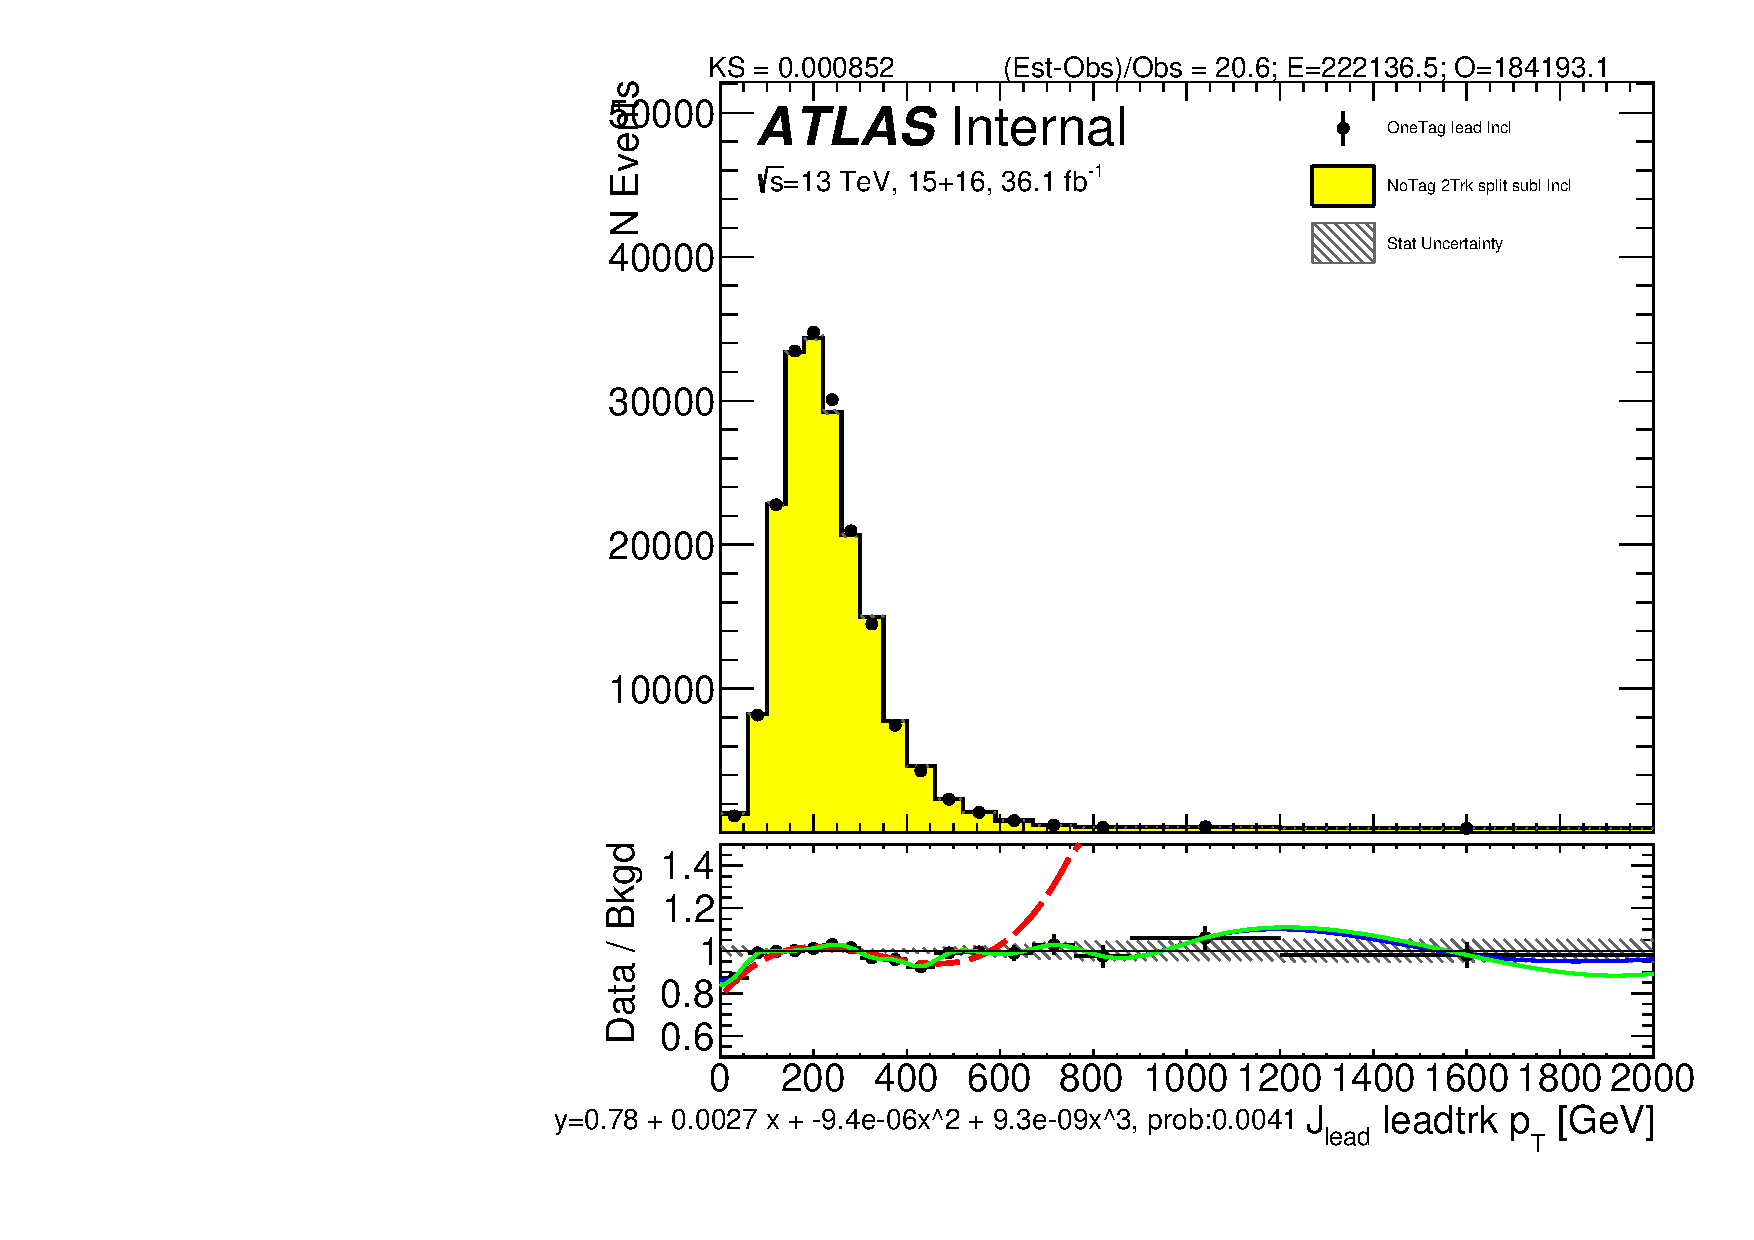
\includegraphics[width=0.25\textwidth,angle=-90]{figures/boosted/Reweight/Fits/Moriond_bkg_0_NoTag_2Trk_split_subl_Incl_leadHCand_trk0_Pt.pdf}
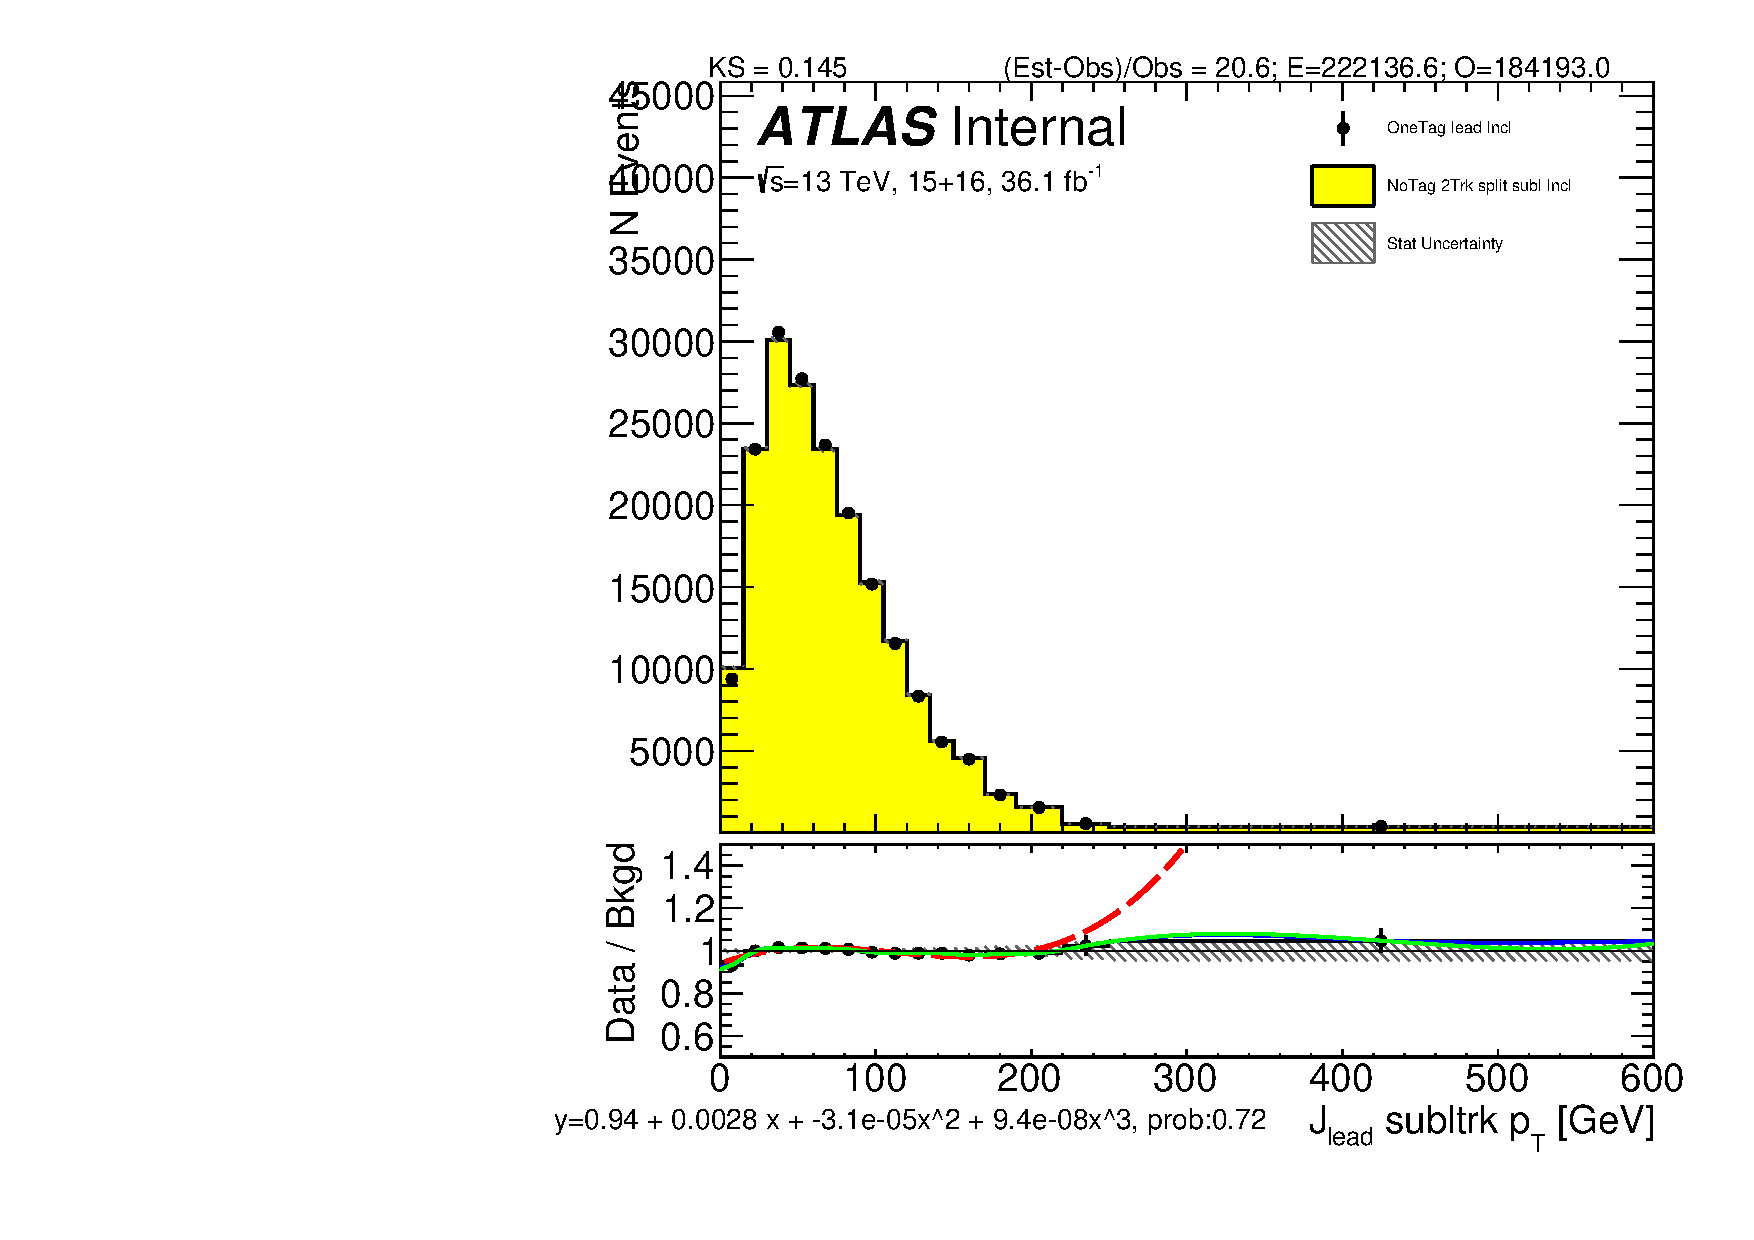
\includegraphics[width=0.25\textwidth,angle=-90]{figures/boosted/Reweight/Fits/Moriond_bkg_0_NoTag_2Trk_split_subl_Incl_leadHCand_trk1_Pt.pdf} \\
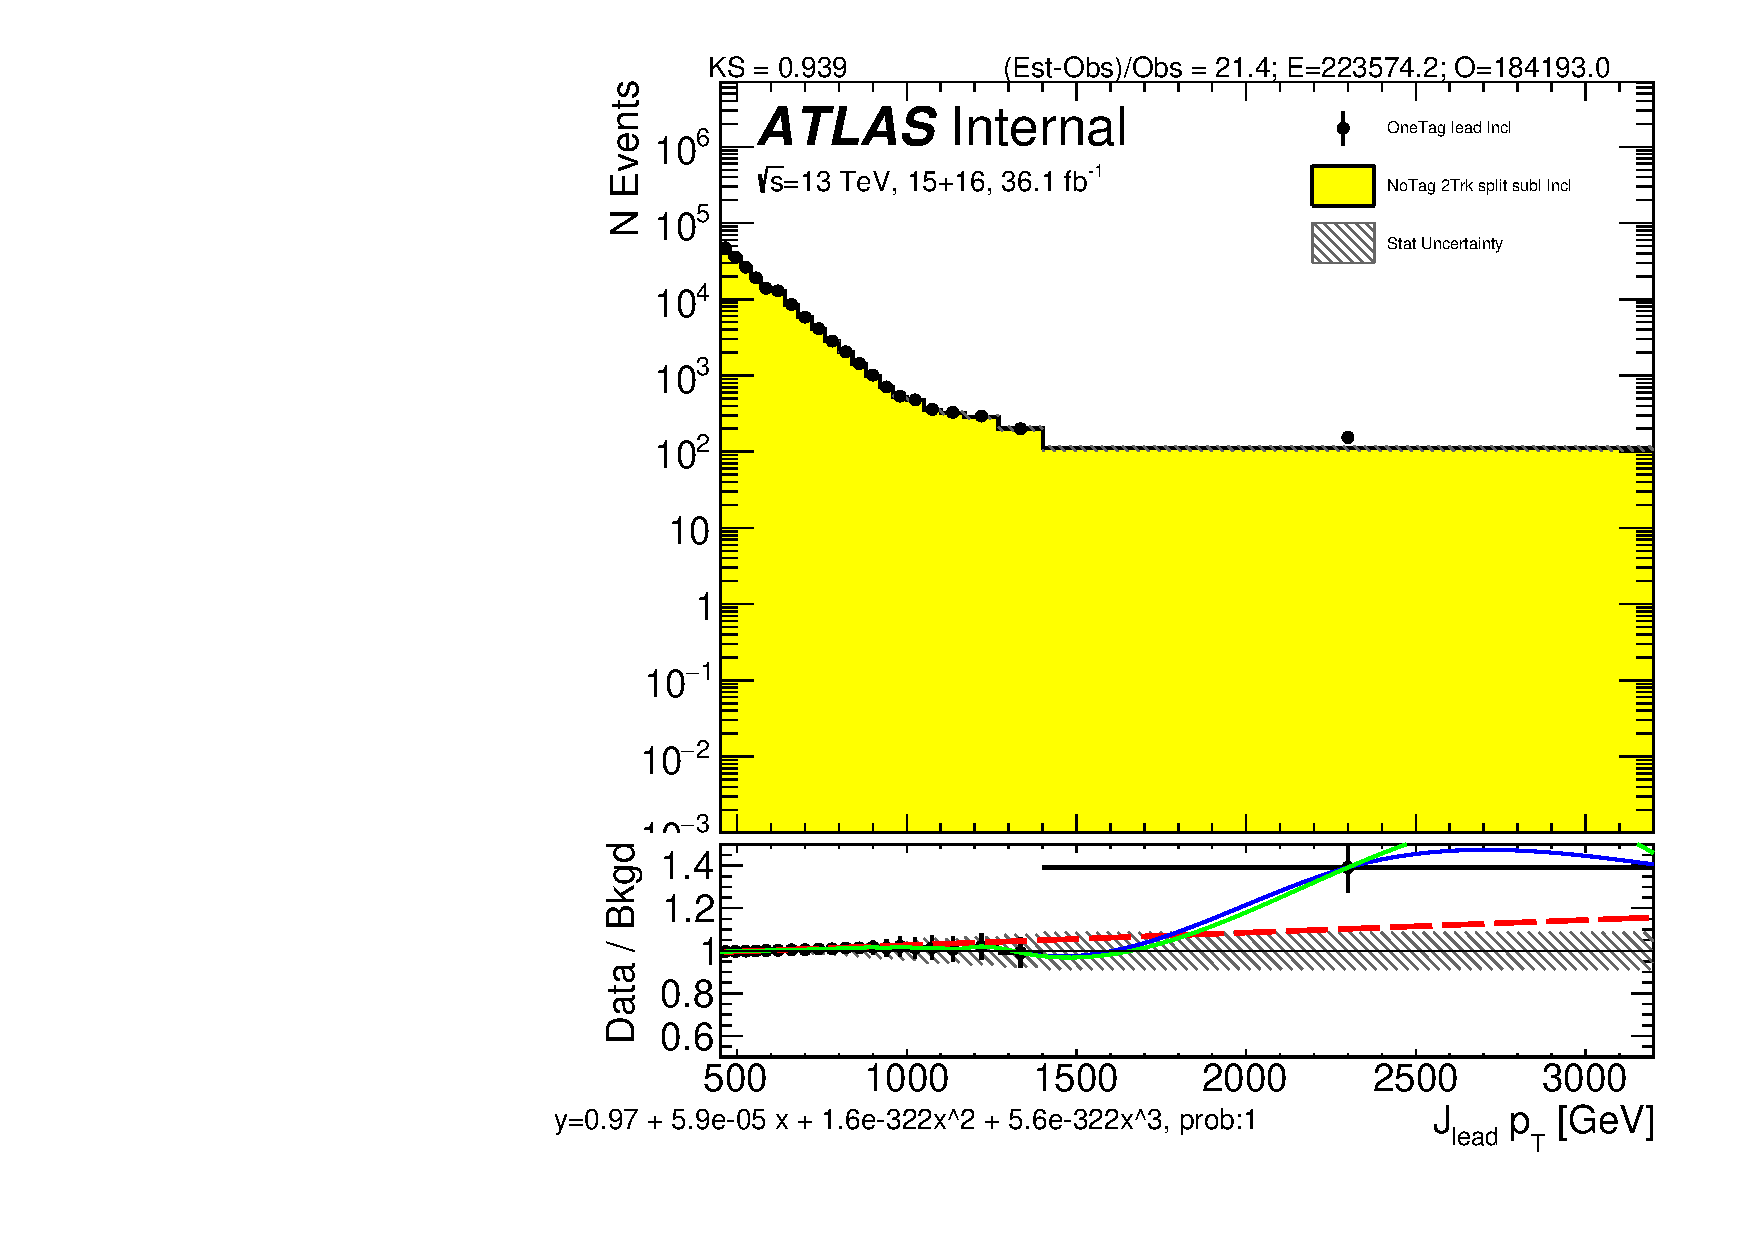
\includegraphics[width=0.25\textwidth,angle=-90]{figures/boosted/Reweight/Fits/Moriond_bkg_3_NoTag_2Trk_split_subl_Incl_leadHCand_Pt_m_1.pdf}
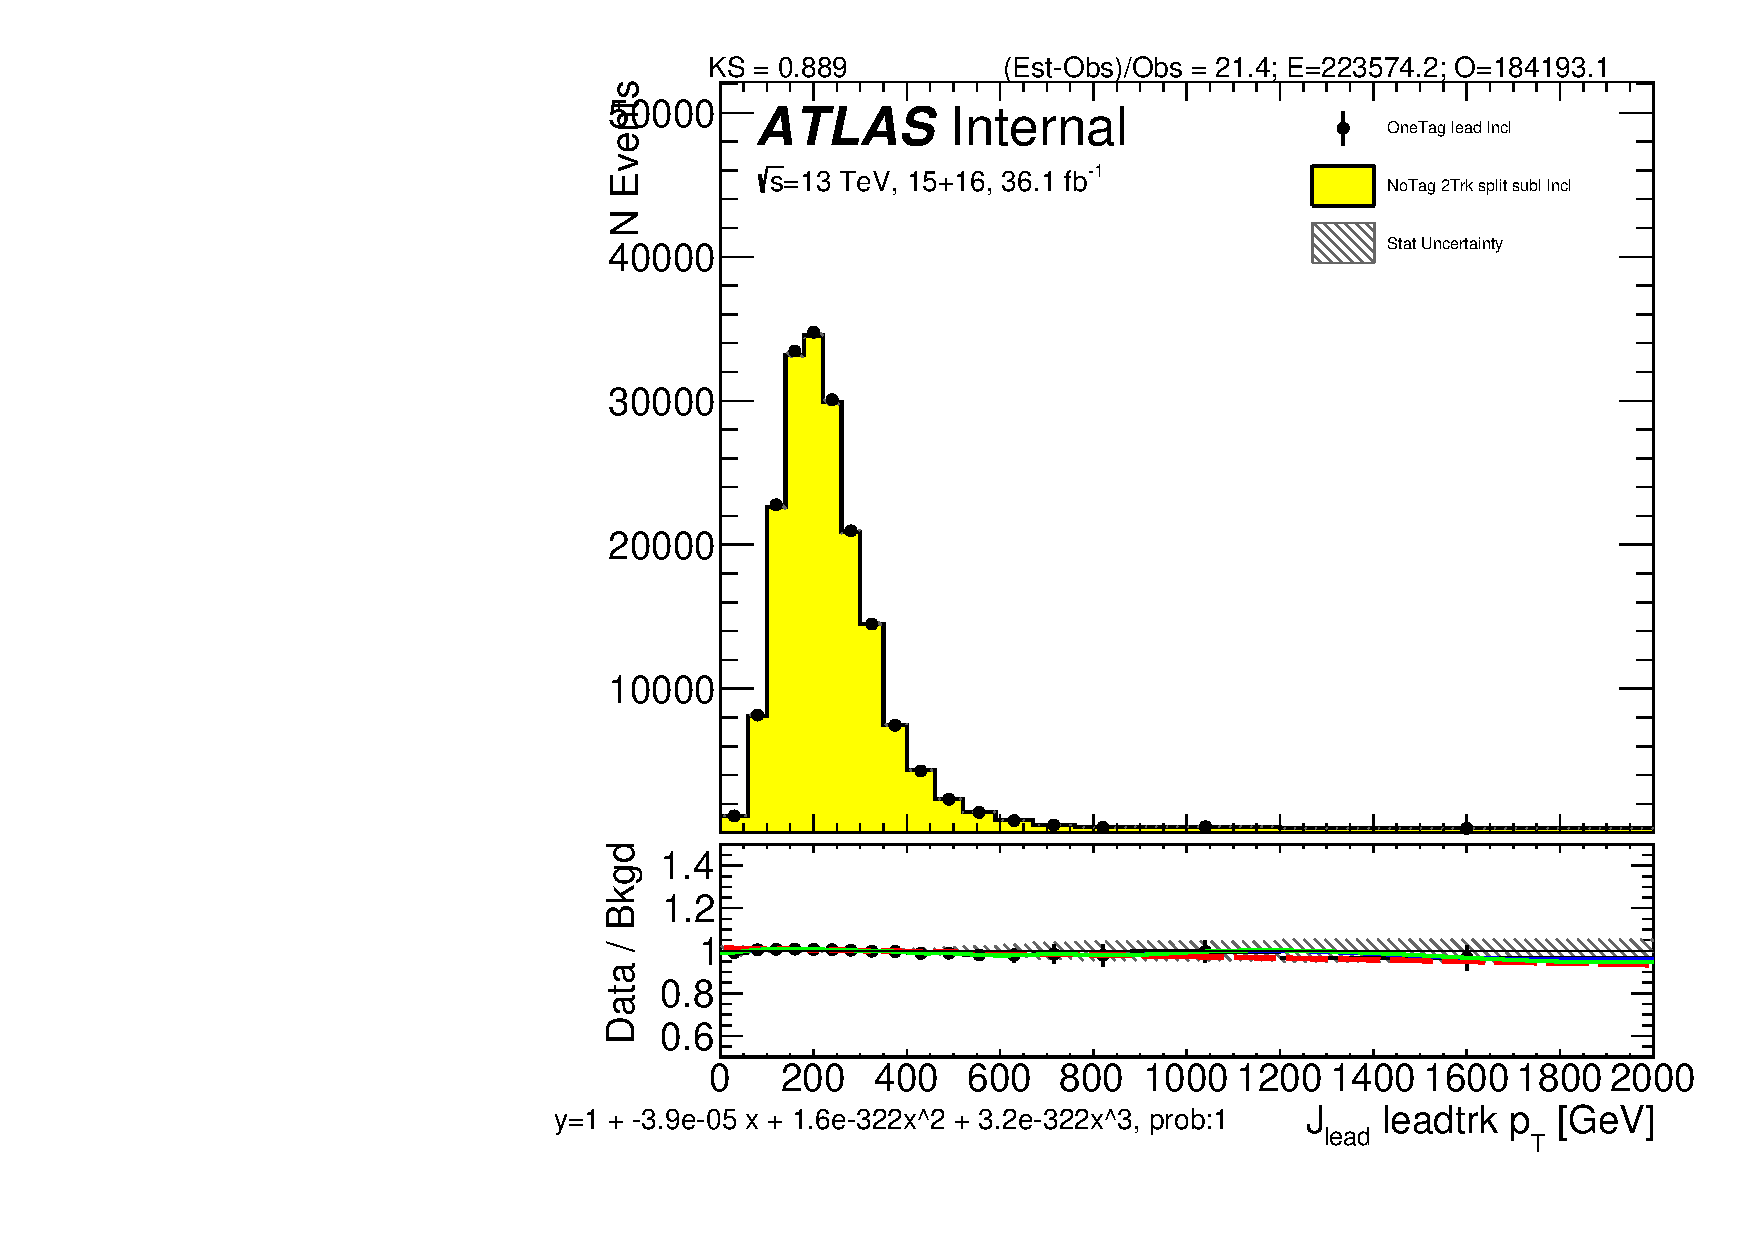
\includegraphics[width=0.25\textwidth,angle=-90]{figures/boosted/Reweight/Fits/Moriond_bkg_3_NoTag_2Trk_split_subl_Incl_leadHCand_trk0_Pt.pdf}
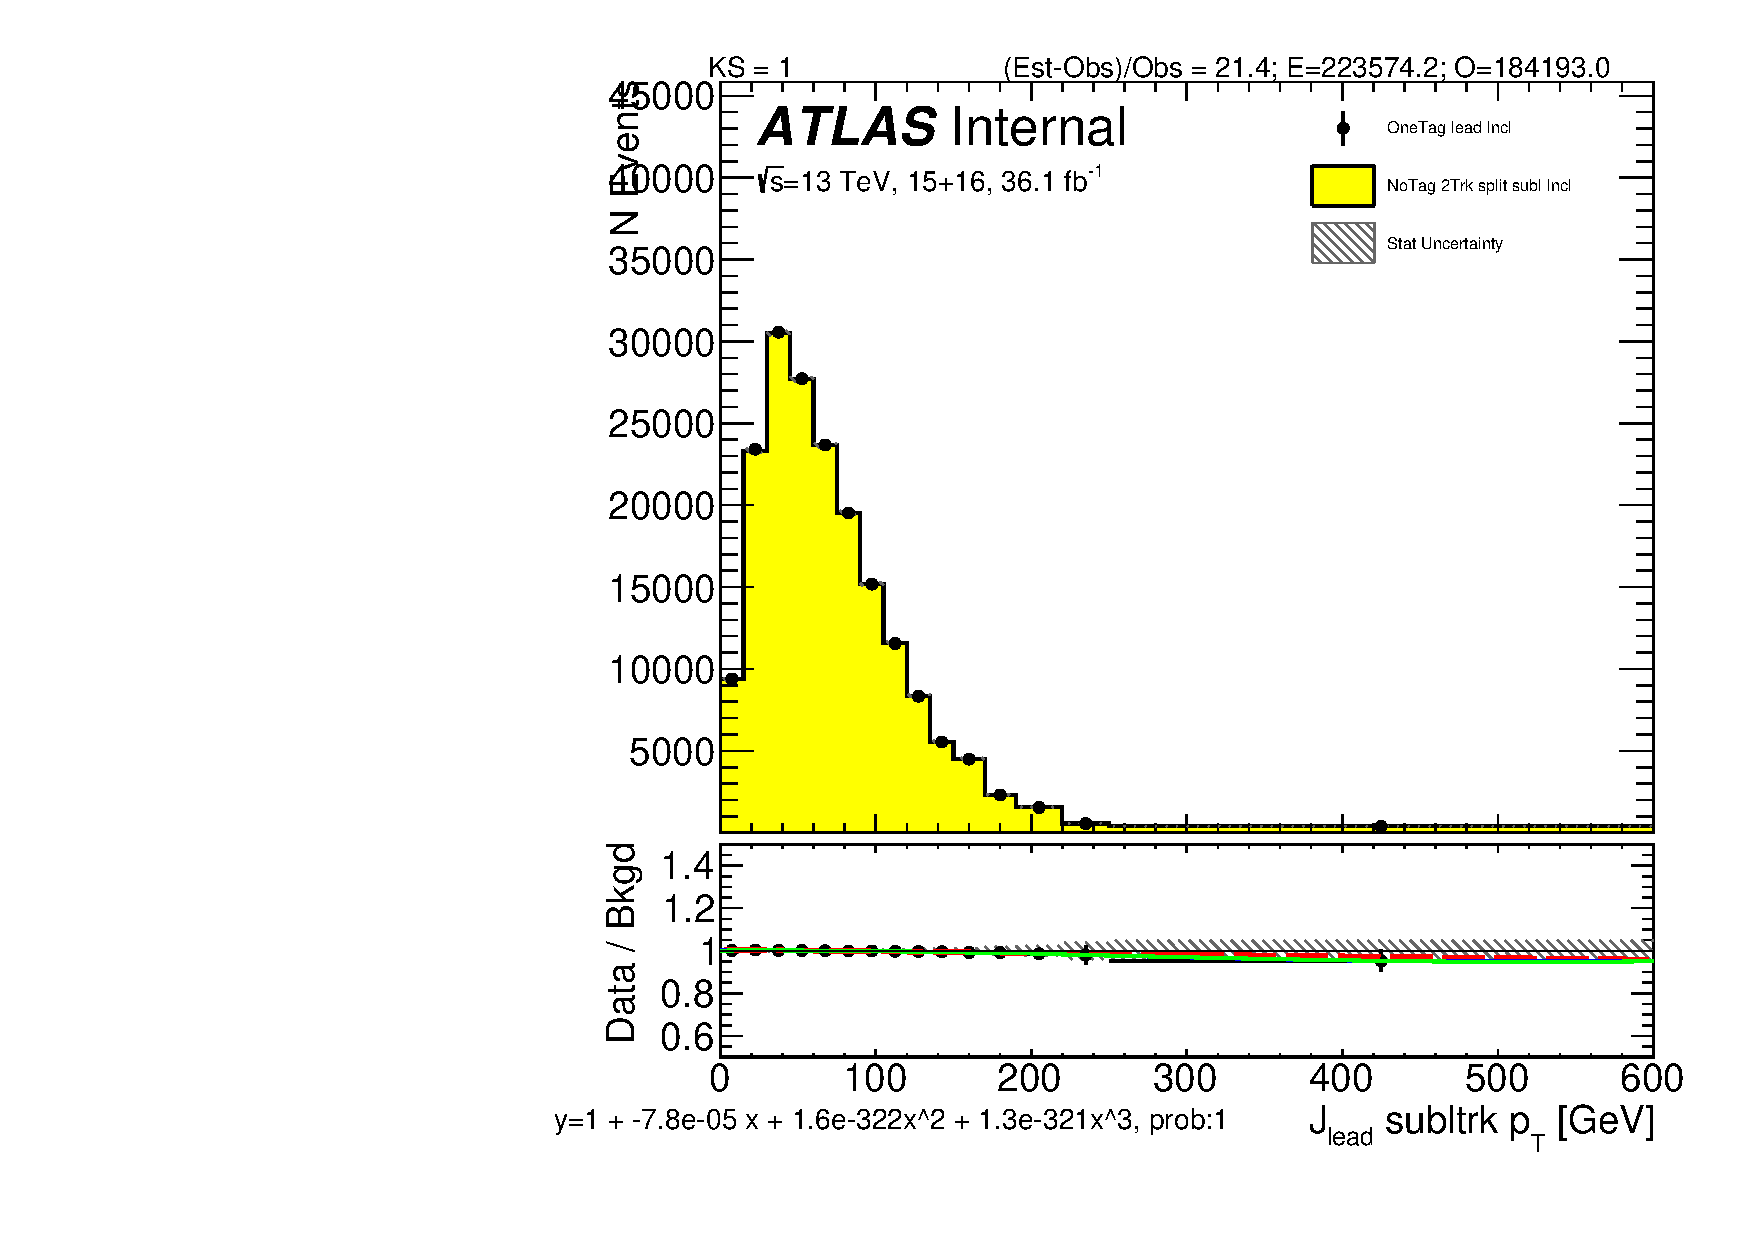
\includegraphics[width=0.25\textwidth,angle=-90]{figures/boosted/Reweight/Fits/Moriond_bkg_3_NoTag_2Trk_split_subl_Incl_leadHCand_trk1_Pt.pdf} \\
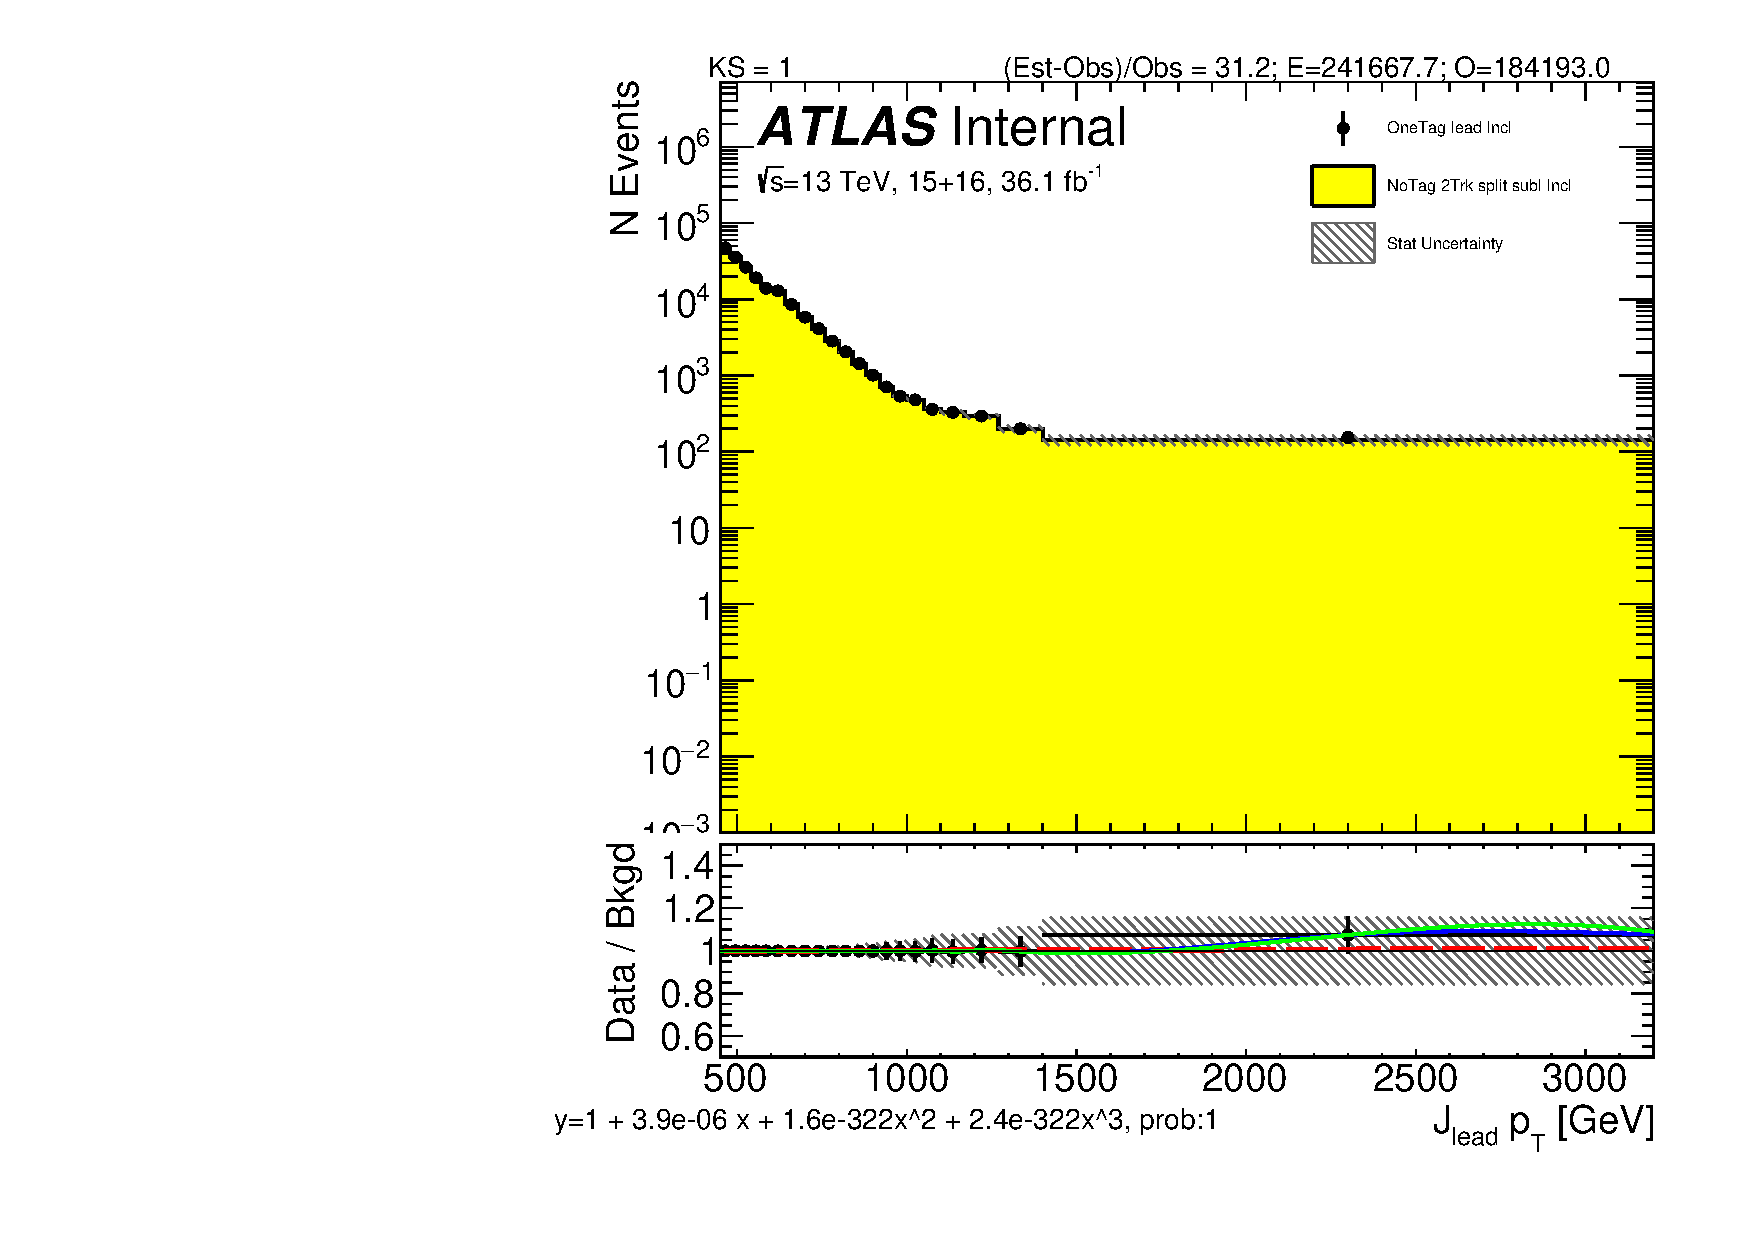
\includegraphics[width=0.25\textwidth,angle=-90]{figures/boosted/Reweight/Fits/Moriond_bkg_9_NoTag_2Trk_split_subl_Incl_leadHCand_Pt_m_1.pdf}
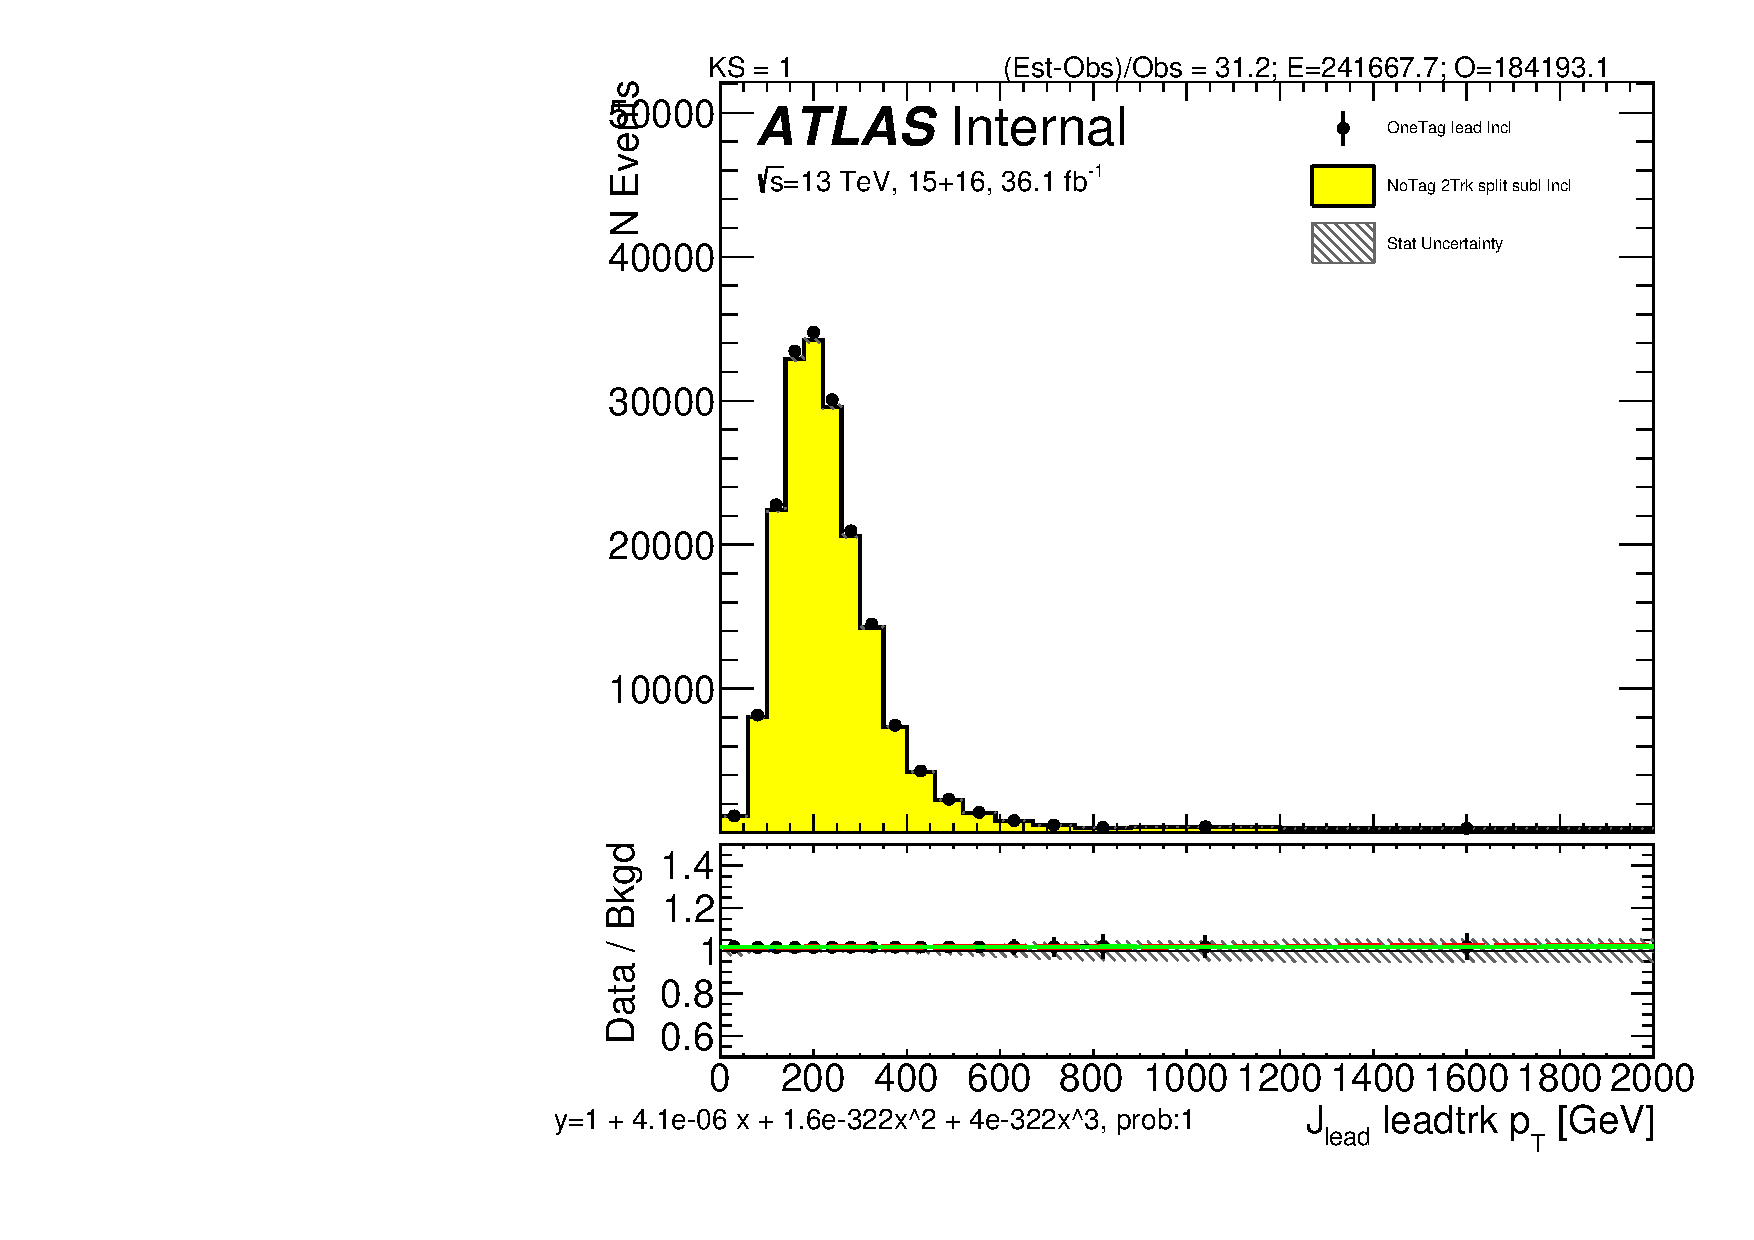
\includegraphics[width=0.25\textwidth,angle=-90]{figures/boosted/Reweight/Fits/Moriond_bkg_9_NoTag_2Trk_split_subl_Incl_leadHCand_trk0_Pt.pdf}
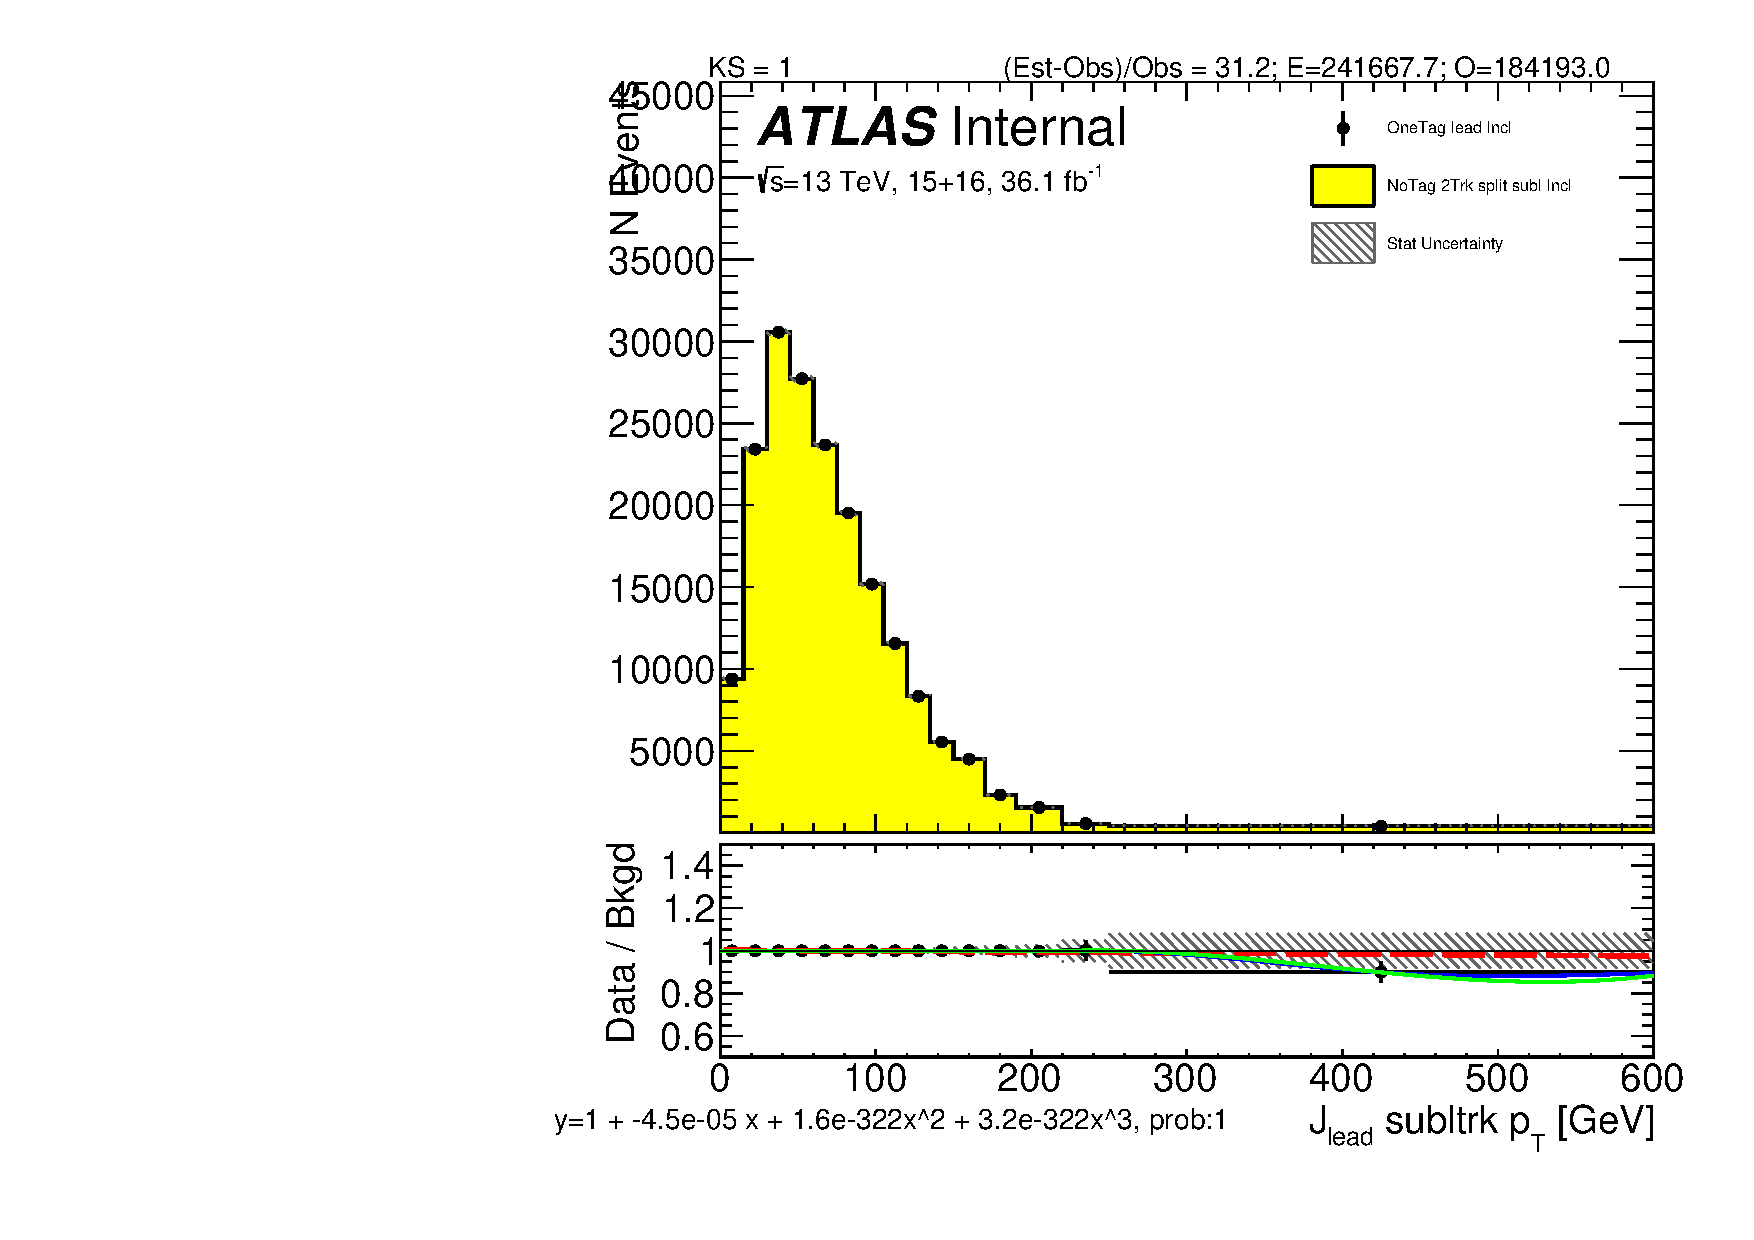
\includegraphics[width=0.25\textwidth,angle=-90]{figures/boosted/Reweight/Fits/Moriond_bkg_9_NoTag_2Trk_split_subl_Incl_leadHCand_trk1_Pt.pdf} \\
\caption{For $2bs$ background estimate: the fits to the ratio of the data in the $1b$ category, of the leading Higgs candidate $1b$-tagged events' leading Higgs candidate distributions(black point), over the subleading Higgs candidate $1b$-tagged events' leading Higgs candidate distributions(yellow). Distributions and fits to the estimated QCD background for large-\R jet $p_{T}$ (left),  the large-\R jet's leading track jet $p_T$ (middle), and large-\R jet's subleading track jet $p_T$ (right) are shown.  Figures are before reweighting (top row), after the first iteration(second row), after the fourth iteration(third row), and after the last iteration (bottom row). The green line is the spline fit; the red line is a polynomial fit; the blue line is the spline interpolation.}
\label{fig:rw-2bs-subl}
\end{center}
\end{figure*}

\begin{figure*}[htbp!]
\begin{center}
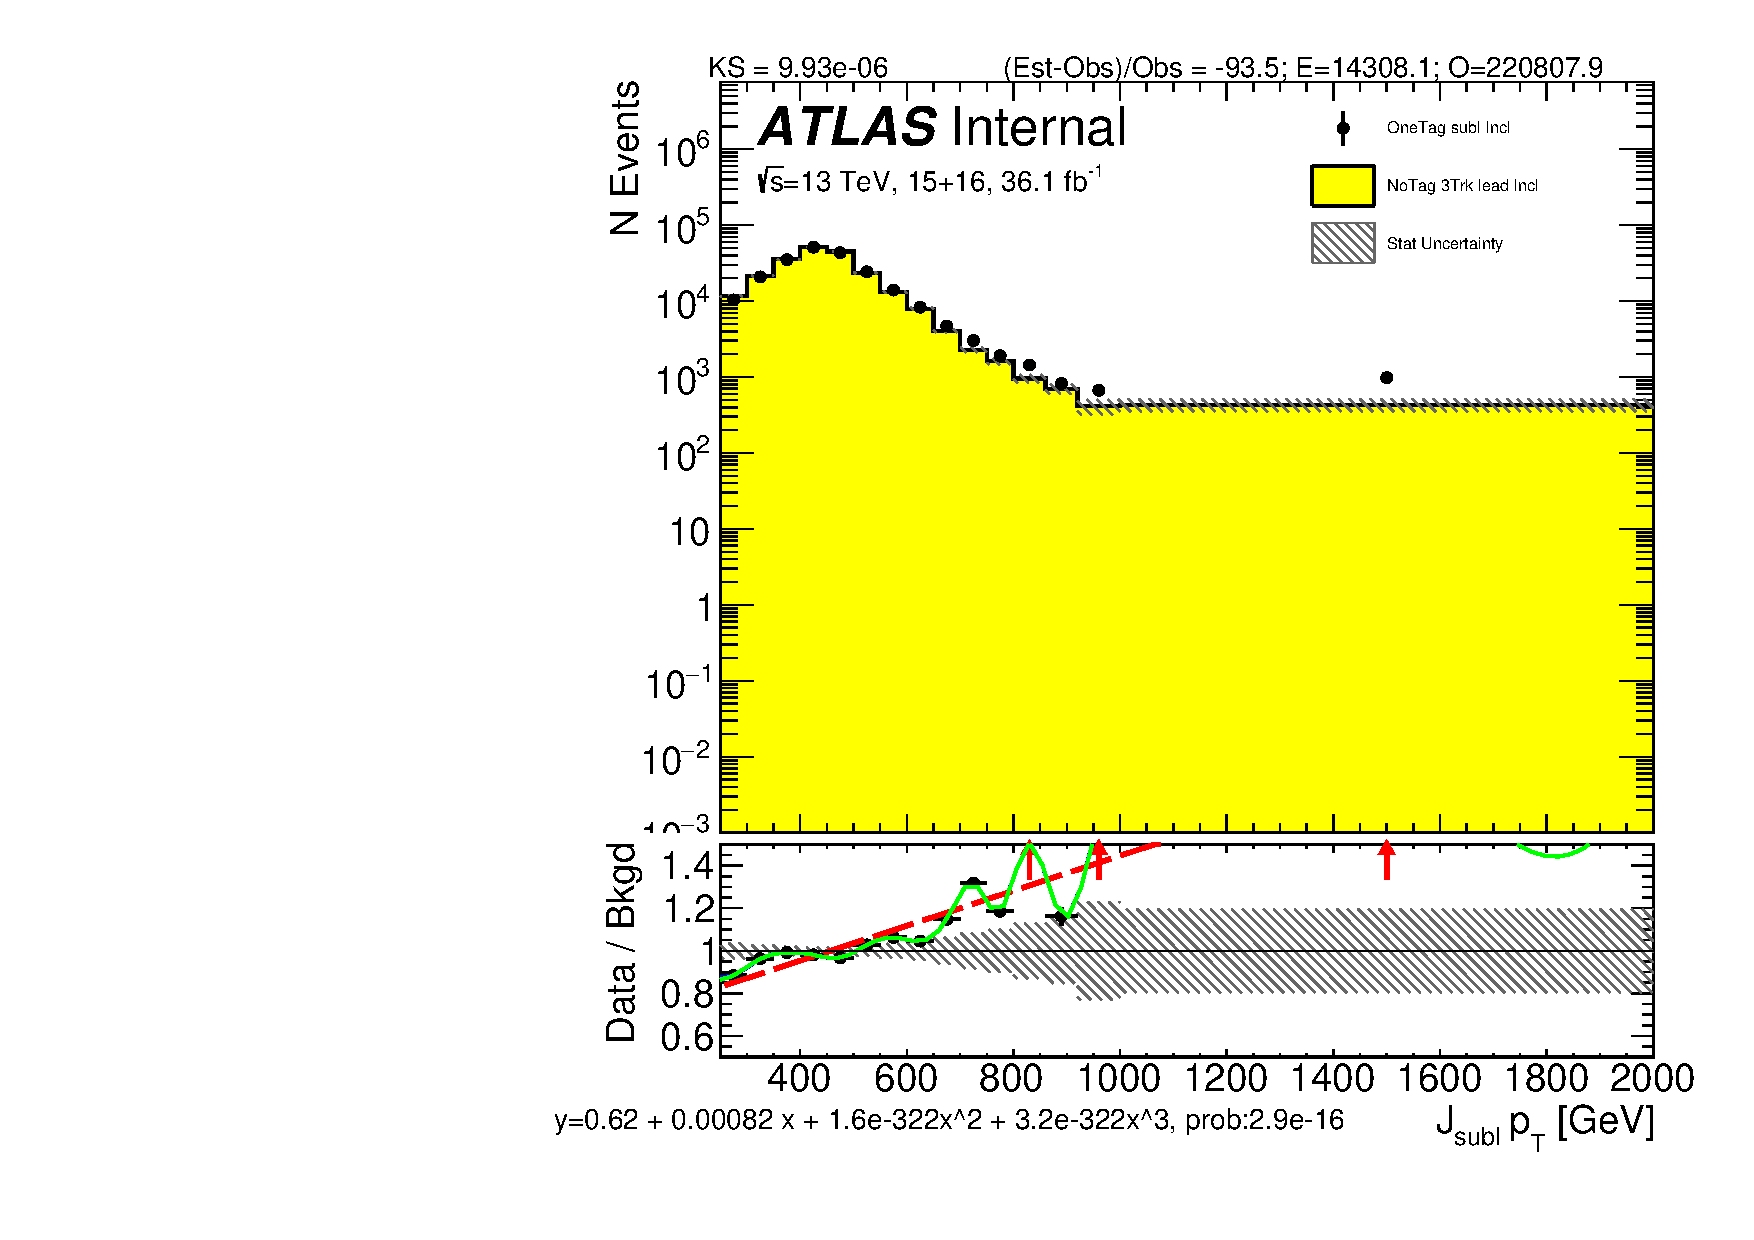
\includegraphics[width=0.25\textwidth,angle=-90]{figures/boosted/Reweight/Fits/Moriond_NoTag_3Trk_lead_Incl_sublHCand_Pt_m_1.pdf}
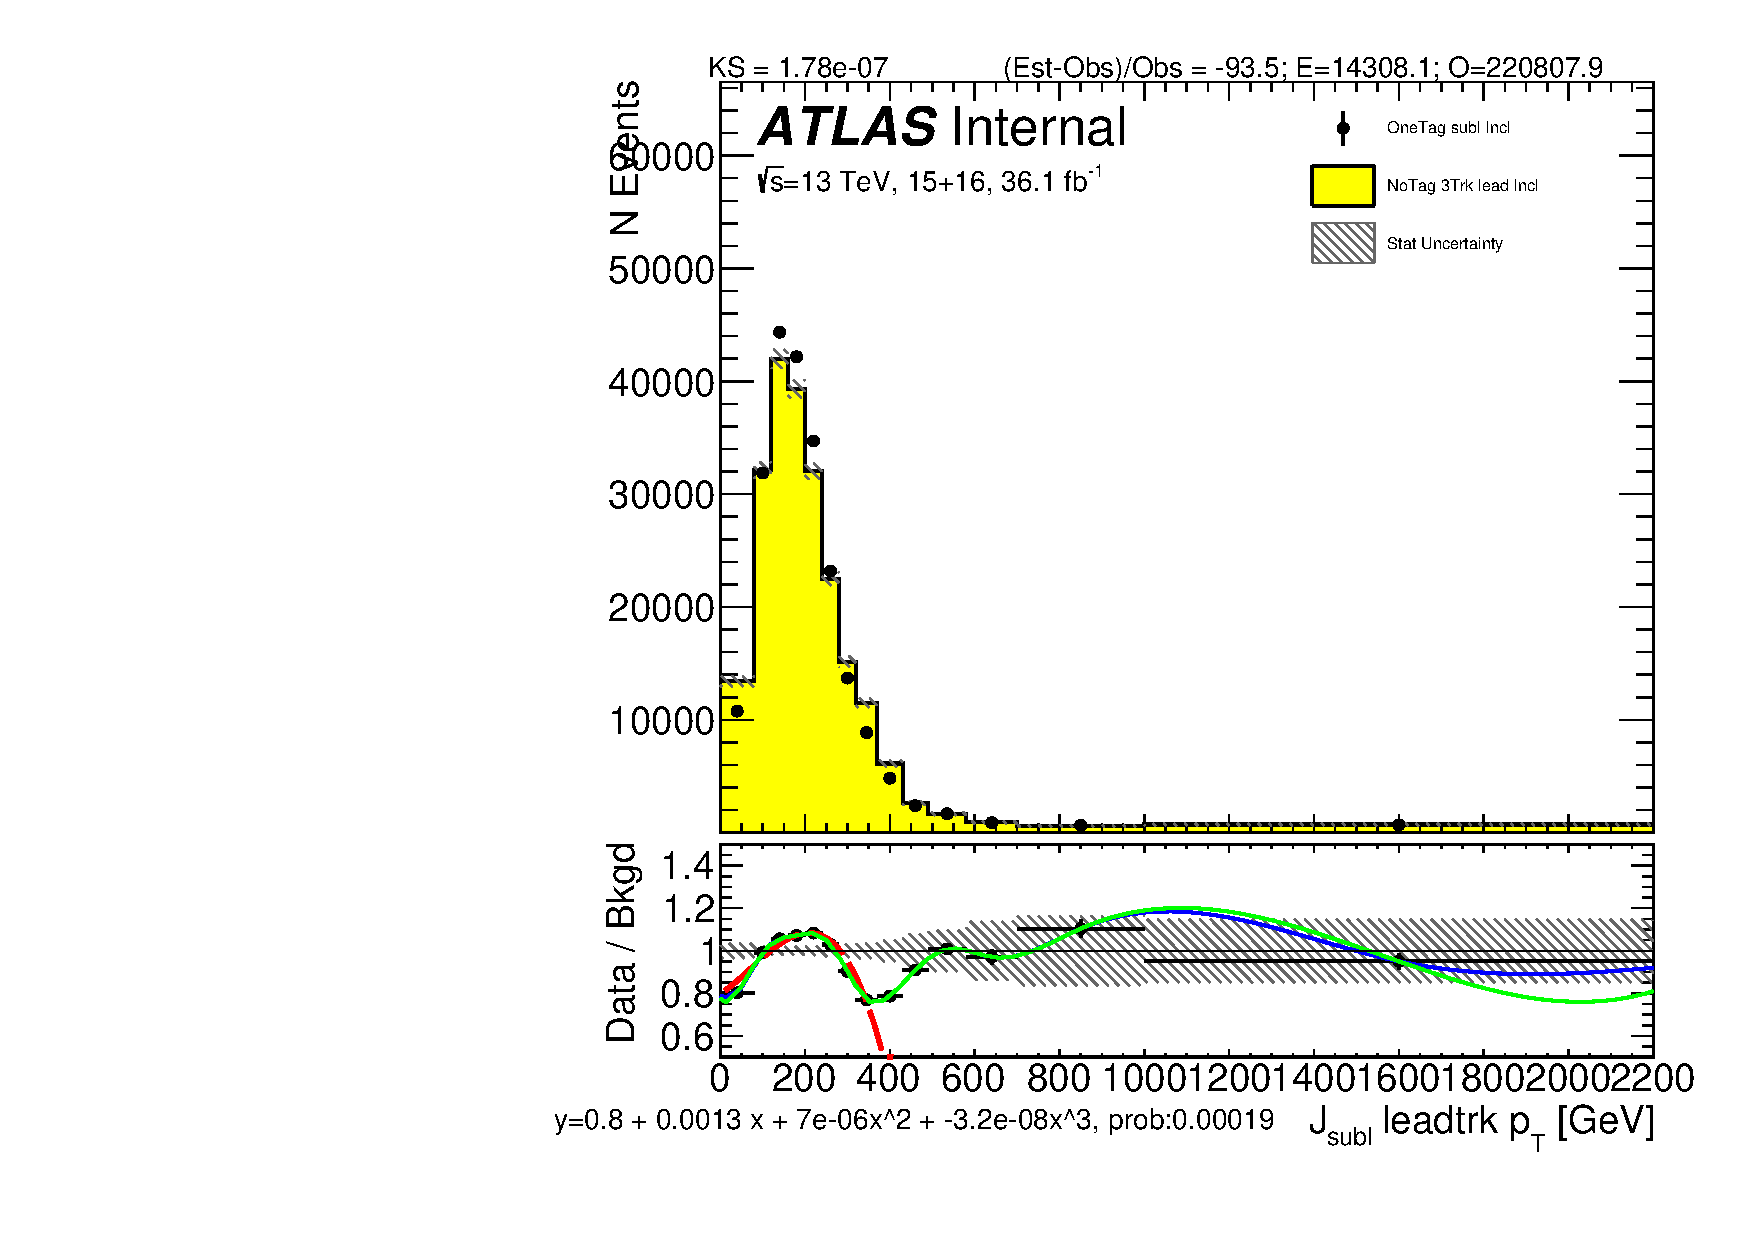
\includegraphics[width=0.25\textwidth,angle=-90]{figures/boosted/Reweight/Fits/Moriond_NoTag_3Trk_lead_Incl_sublHCand_trk0_Pt.pdf}
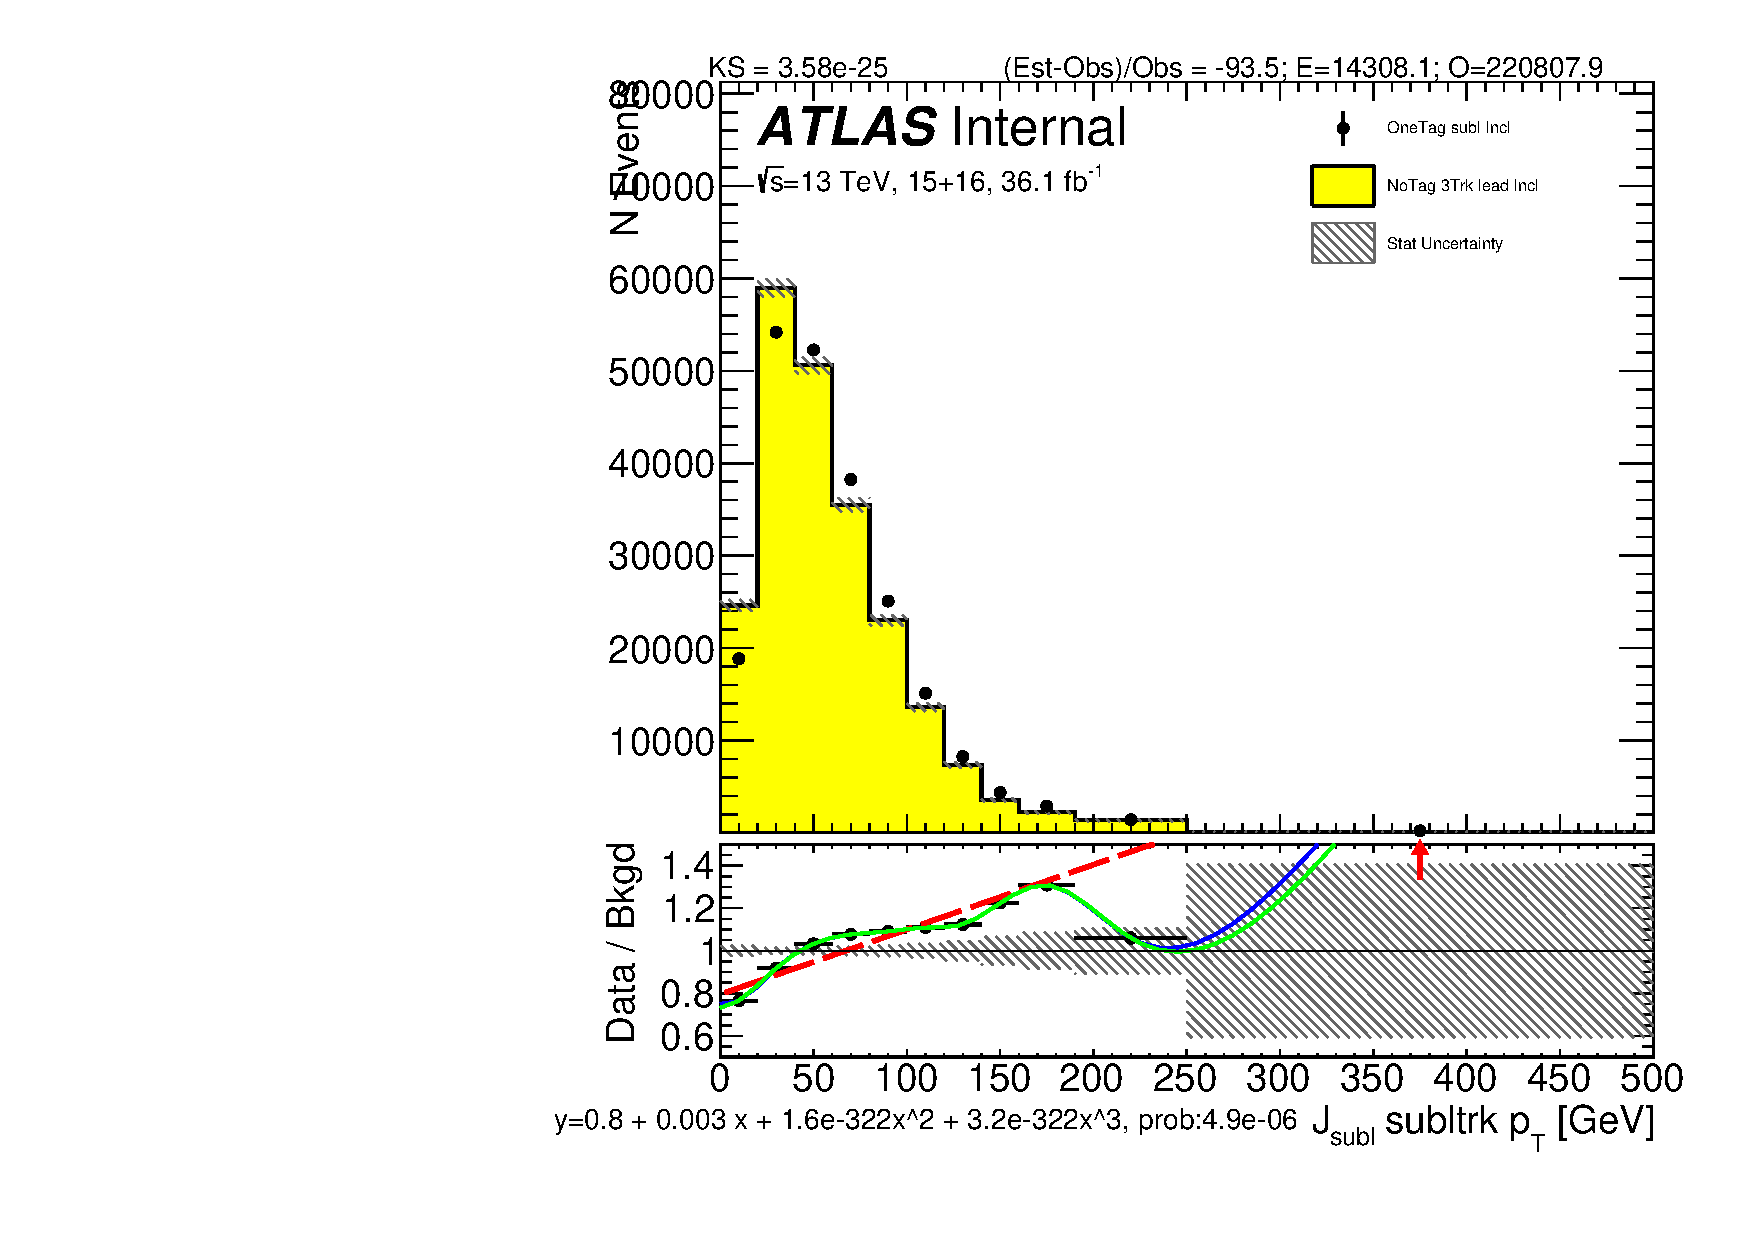
\includegraphics[width=0.25\textwidth,angle=-90]{figures/boosted/Reweight/Fits/Moriond_NoTag_3Trk_lead_Incl_sublHCand_trk1_Pt.pdf} \\
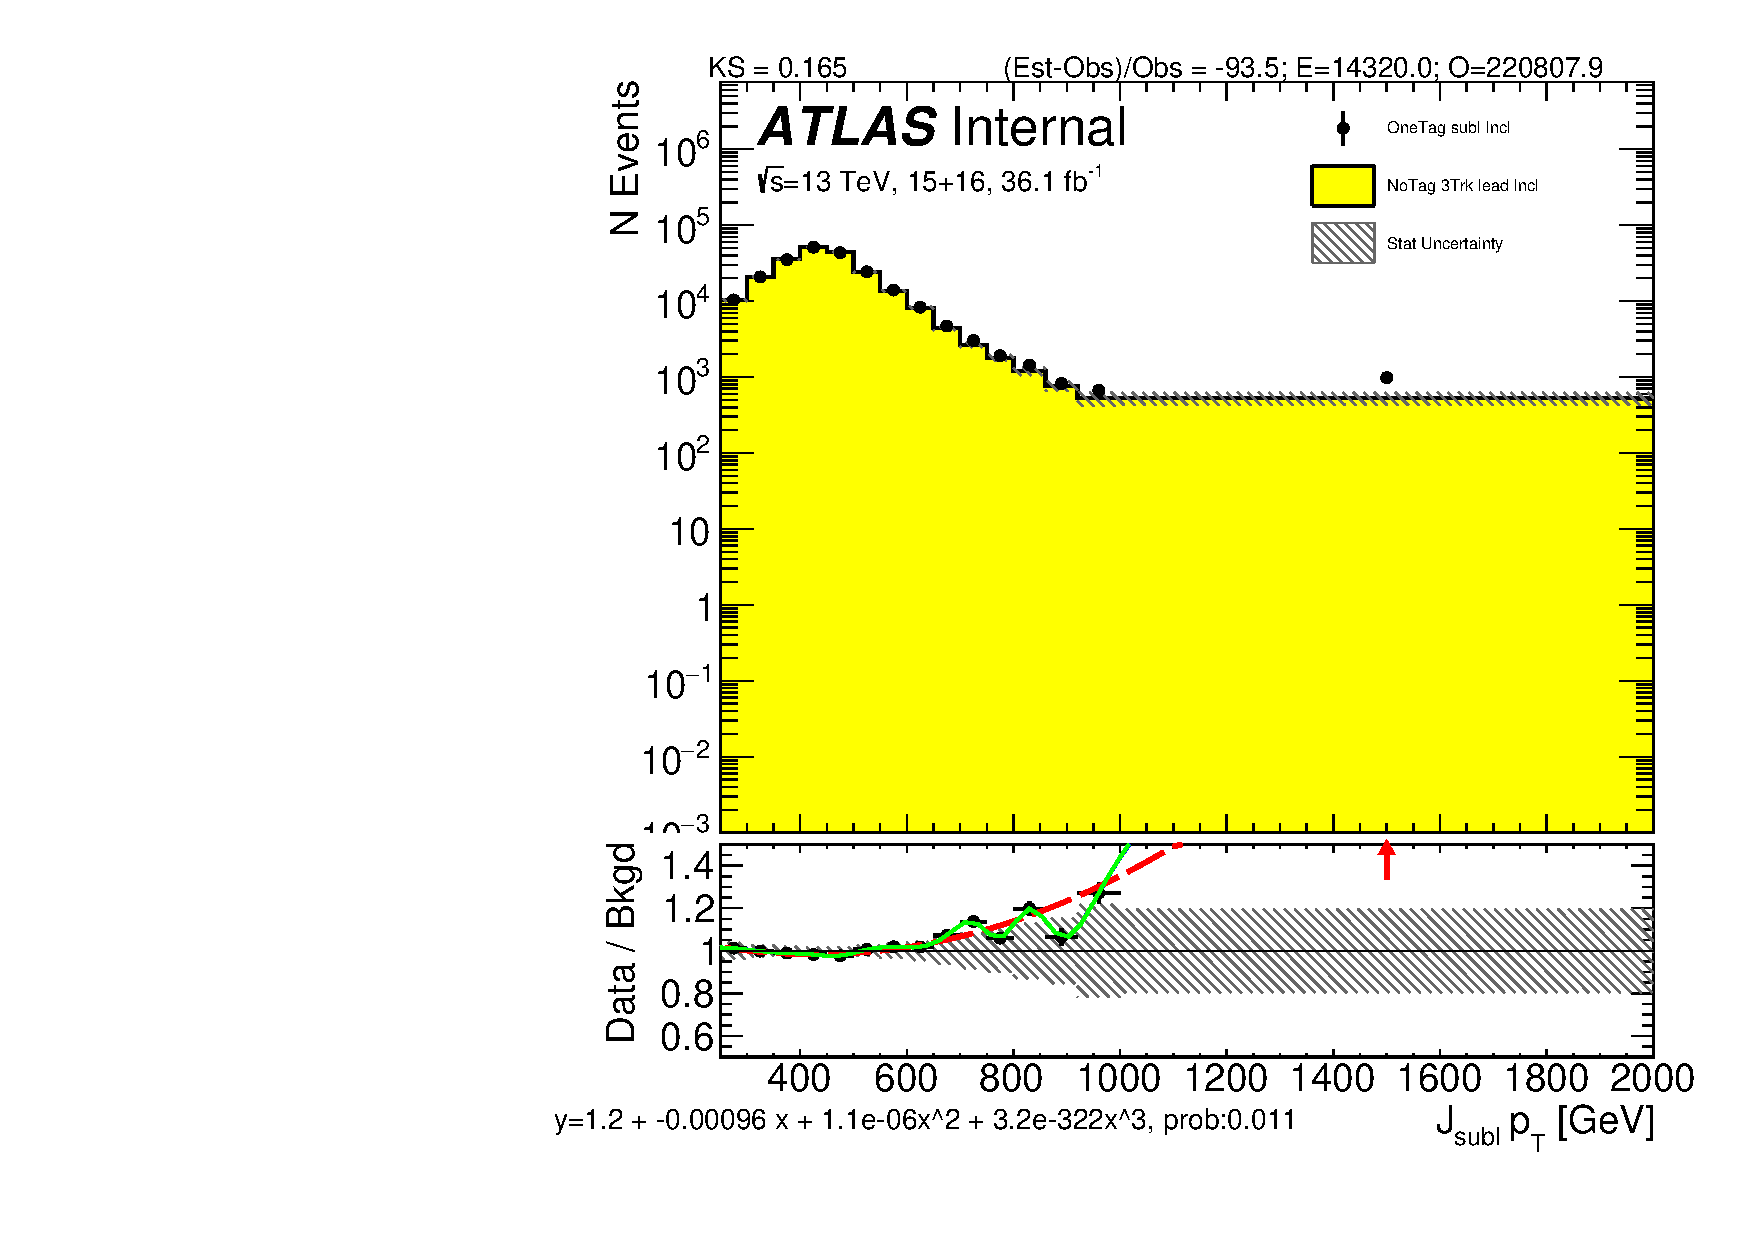
\includegraphics[width=0.25\textwidth,angle=-90]{figures/boosted/Reweight/Fits/Moriond_bkg_0_NoTag_3Trk_lead_Incl_sublHCand_Pt_m_1.pdf}
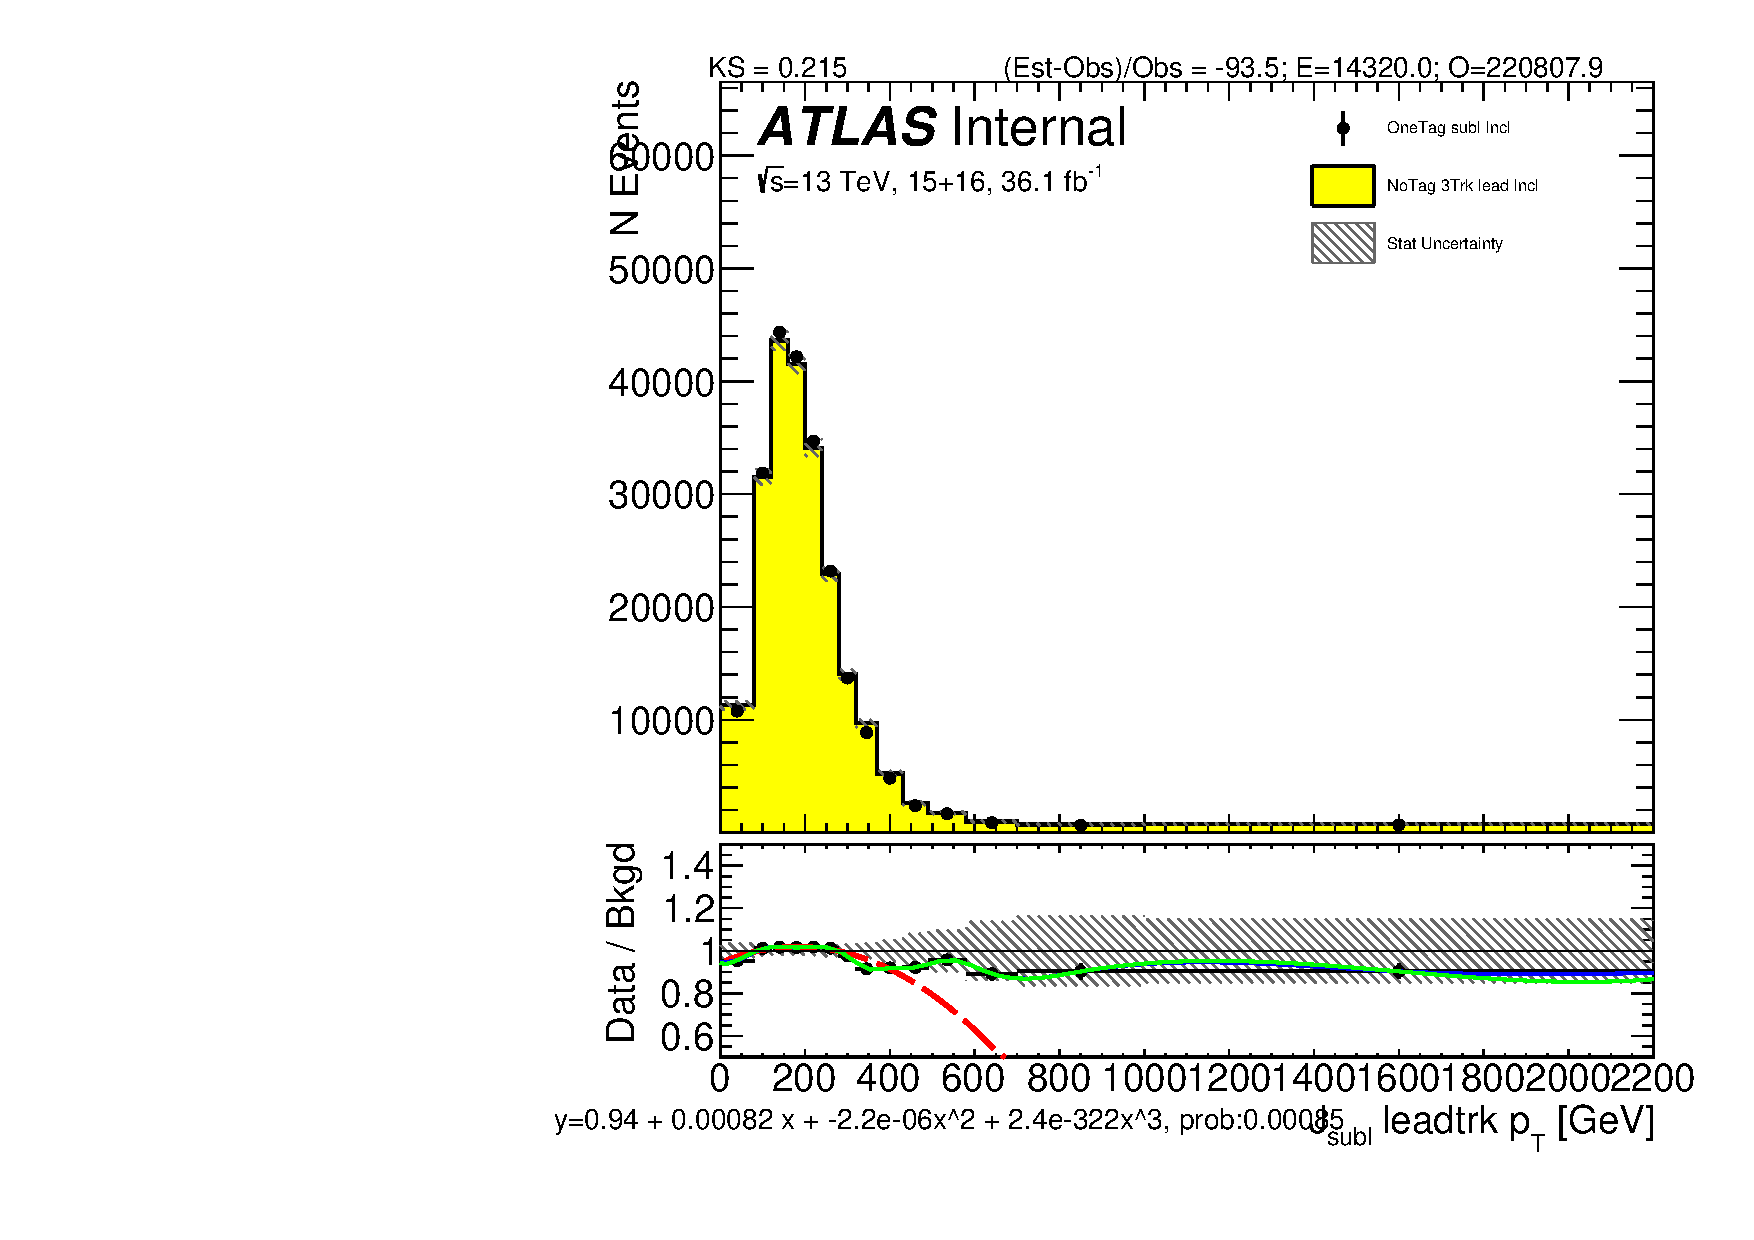
\includegraphics[width=0.25\textwidth,angle=-90]{figures/boosted/Reweight/Fits/Moriond_bkg_0_NoTag_3Trk_lead_Incl_sublHCand_trk0_Pt.pdf}
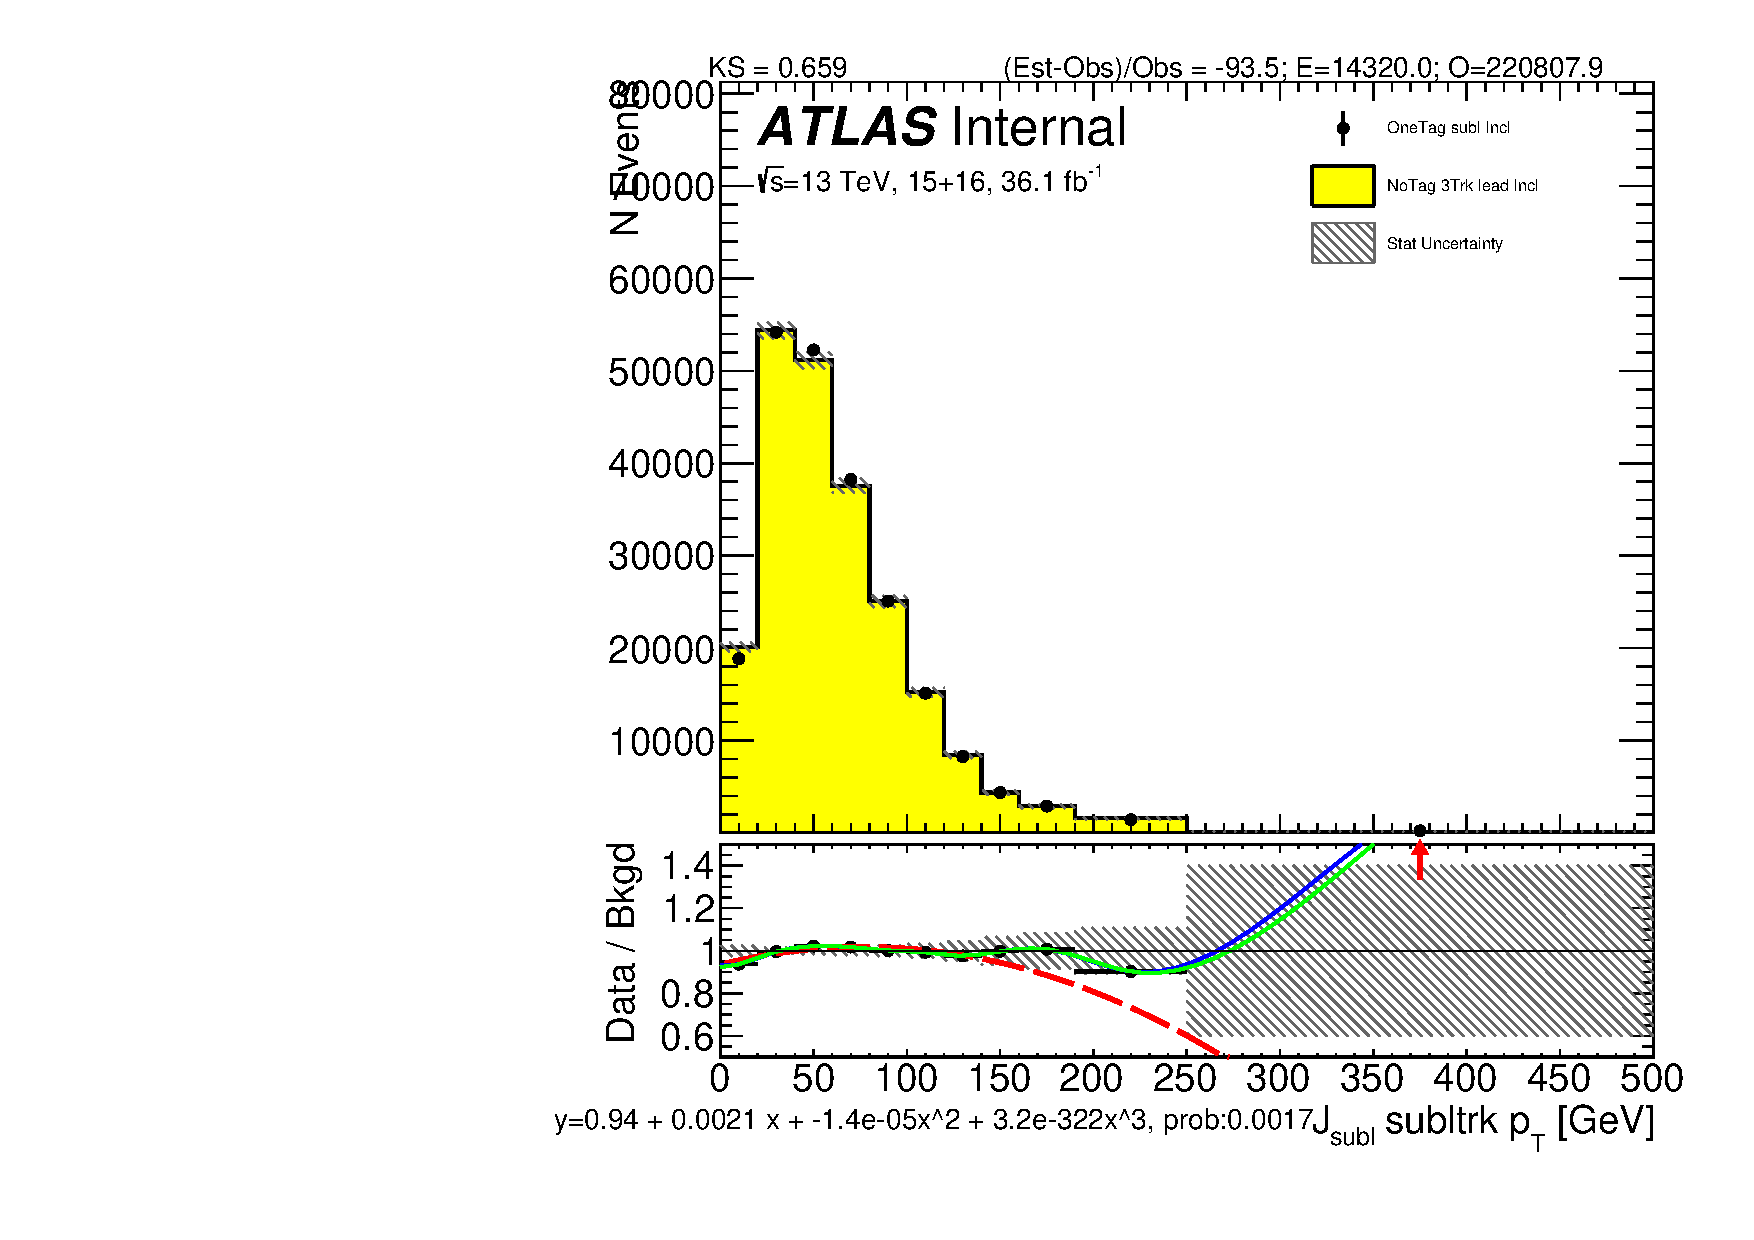
\includegraphics[width=0.25\textwidth,angle=-90]{figures/boosted/Reweight/Fits/Moriond_bkg_0_NoTag_3Trk_lead_Incl_sublHCand_trk1_Pt.pdf} \\
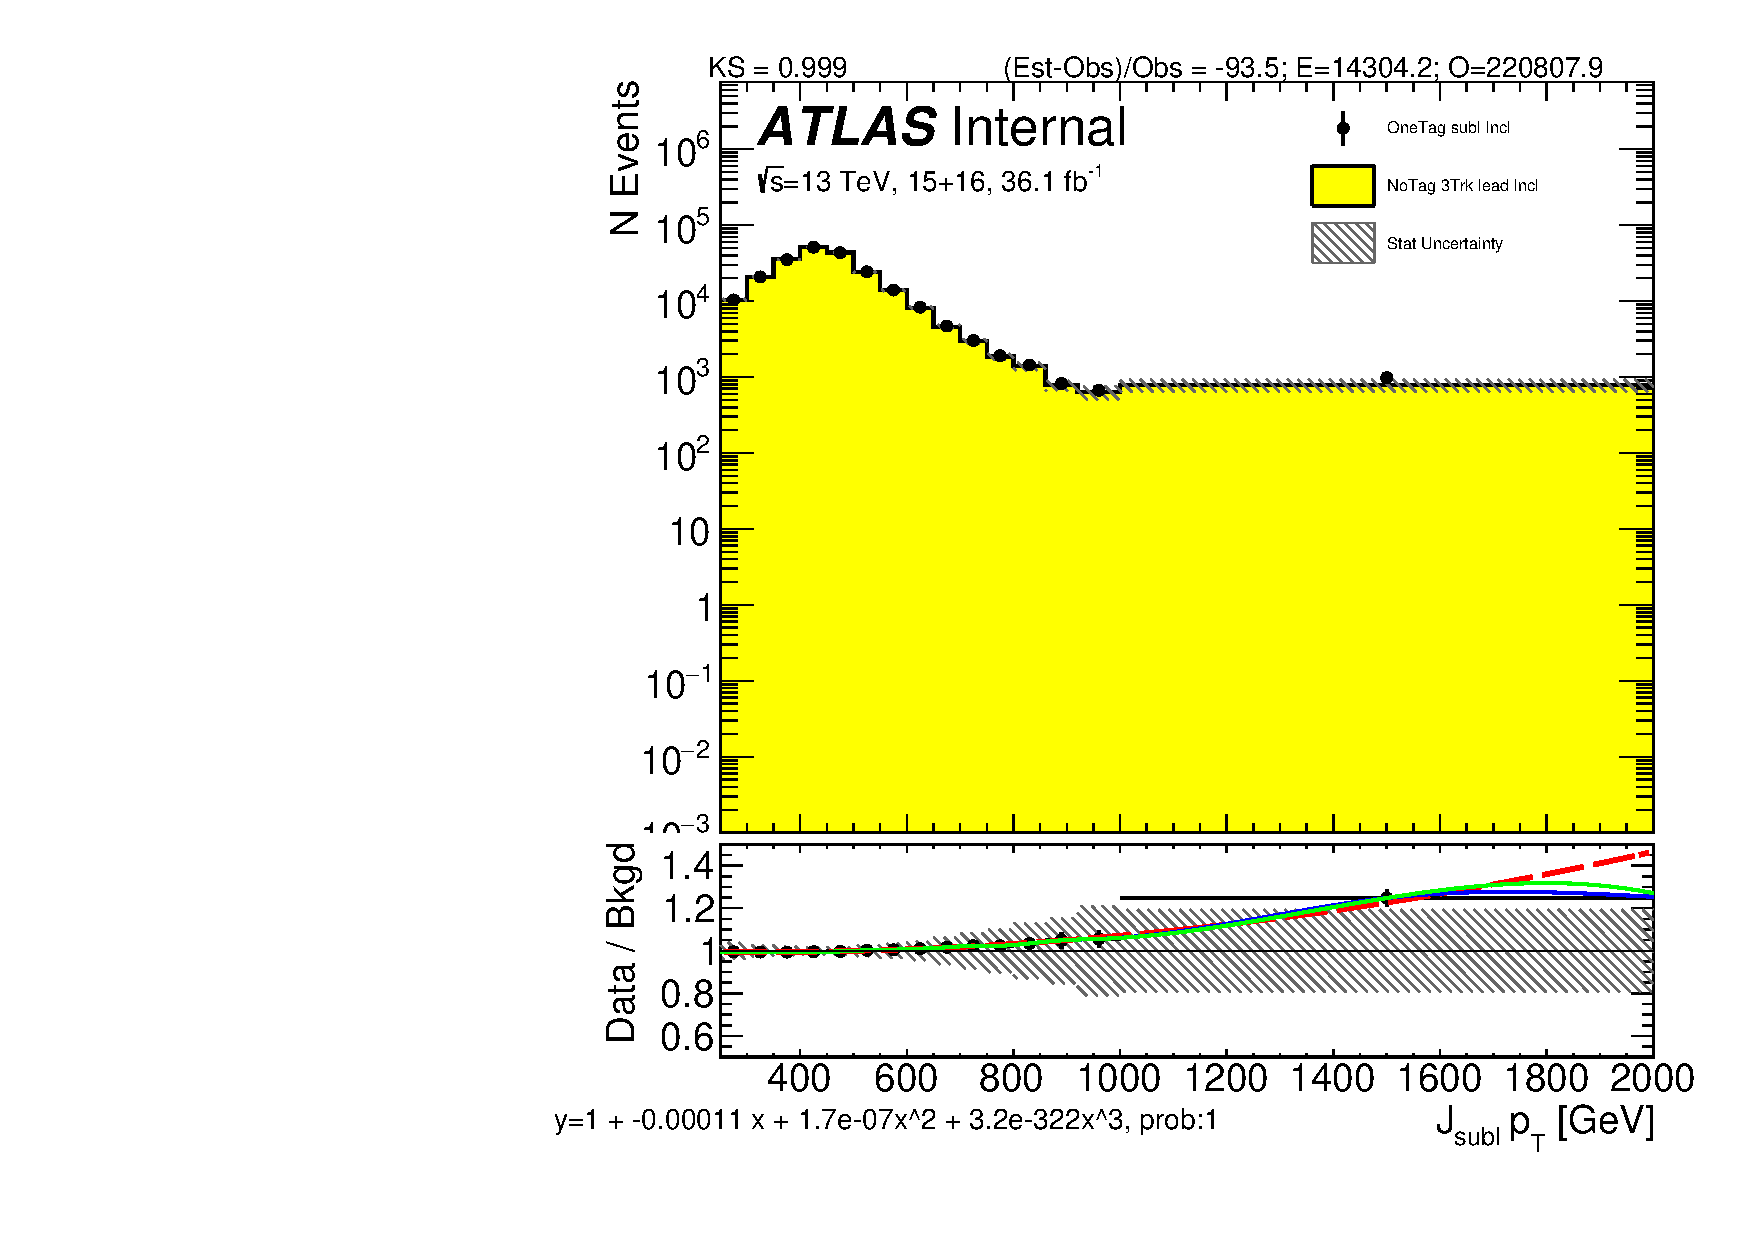
\includegraphics[width=0.25\textwidth,angle=-90]{figures/boosted/Reweight/Fits/Moriond_bkg_3_NoTag_3Trk_lead_Incl_sublHCand_Pt_m_1.pdf}
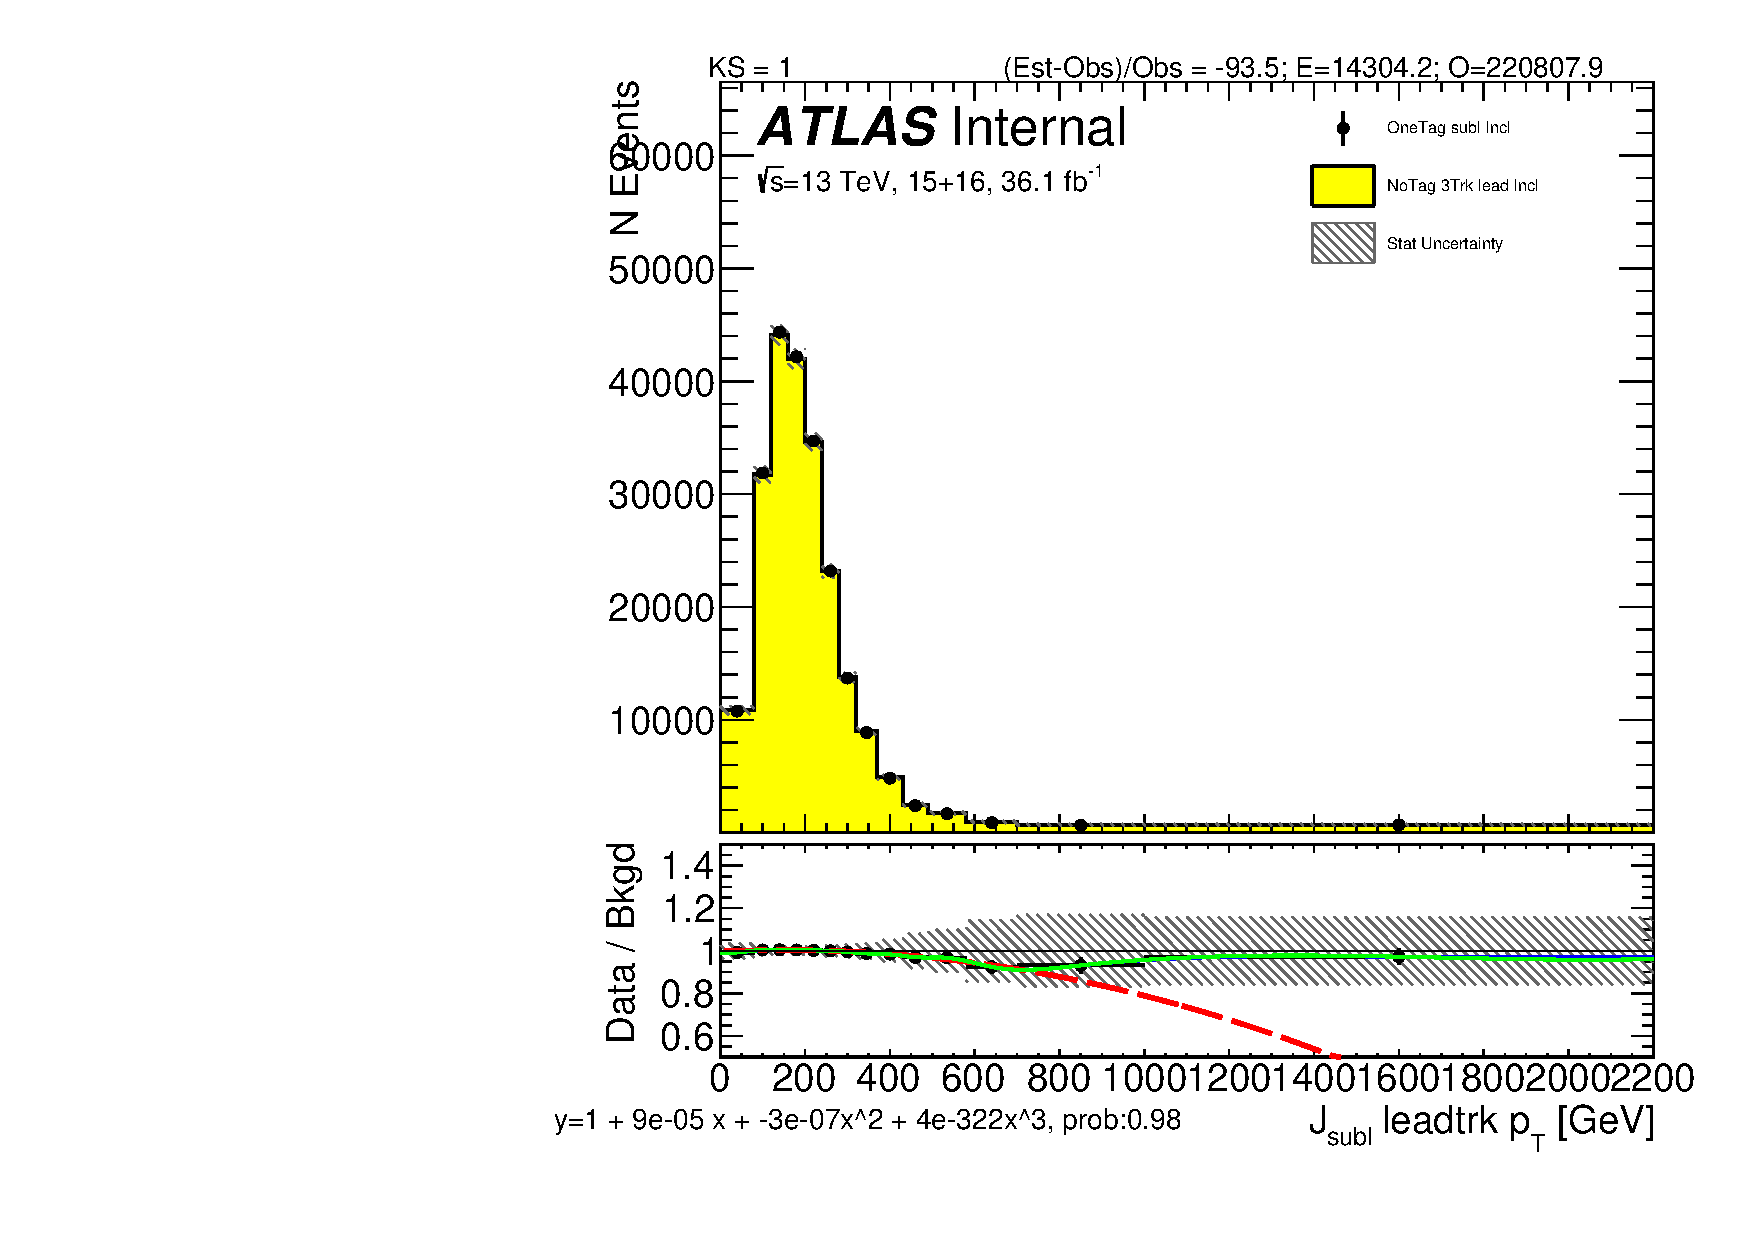
\includegraphics[width=0.25\textwidth,angle=-90]{figures/boosted/Reweight/Fits/Moriond_bkg_3_NoTag_3Trk_lead_Incl_sublHCand_trk0_Pt.pdf}
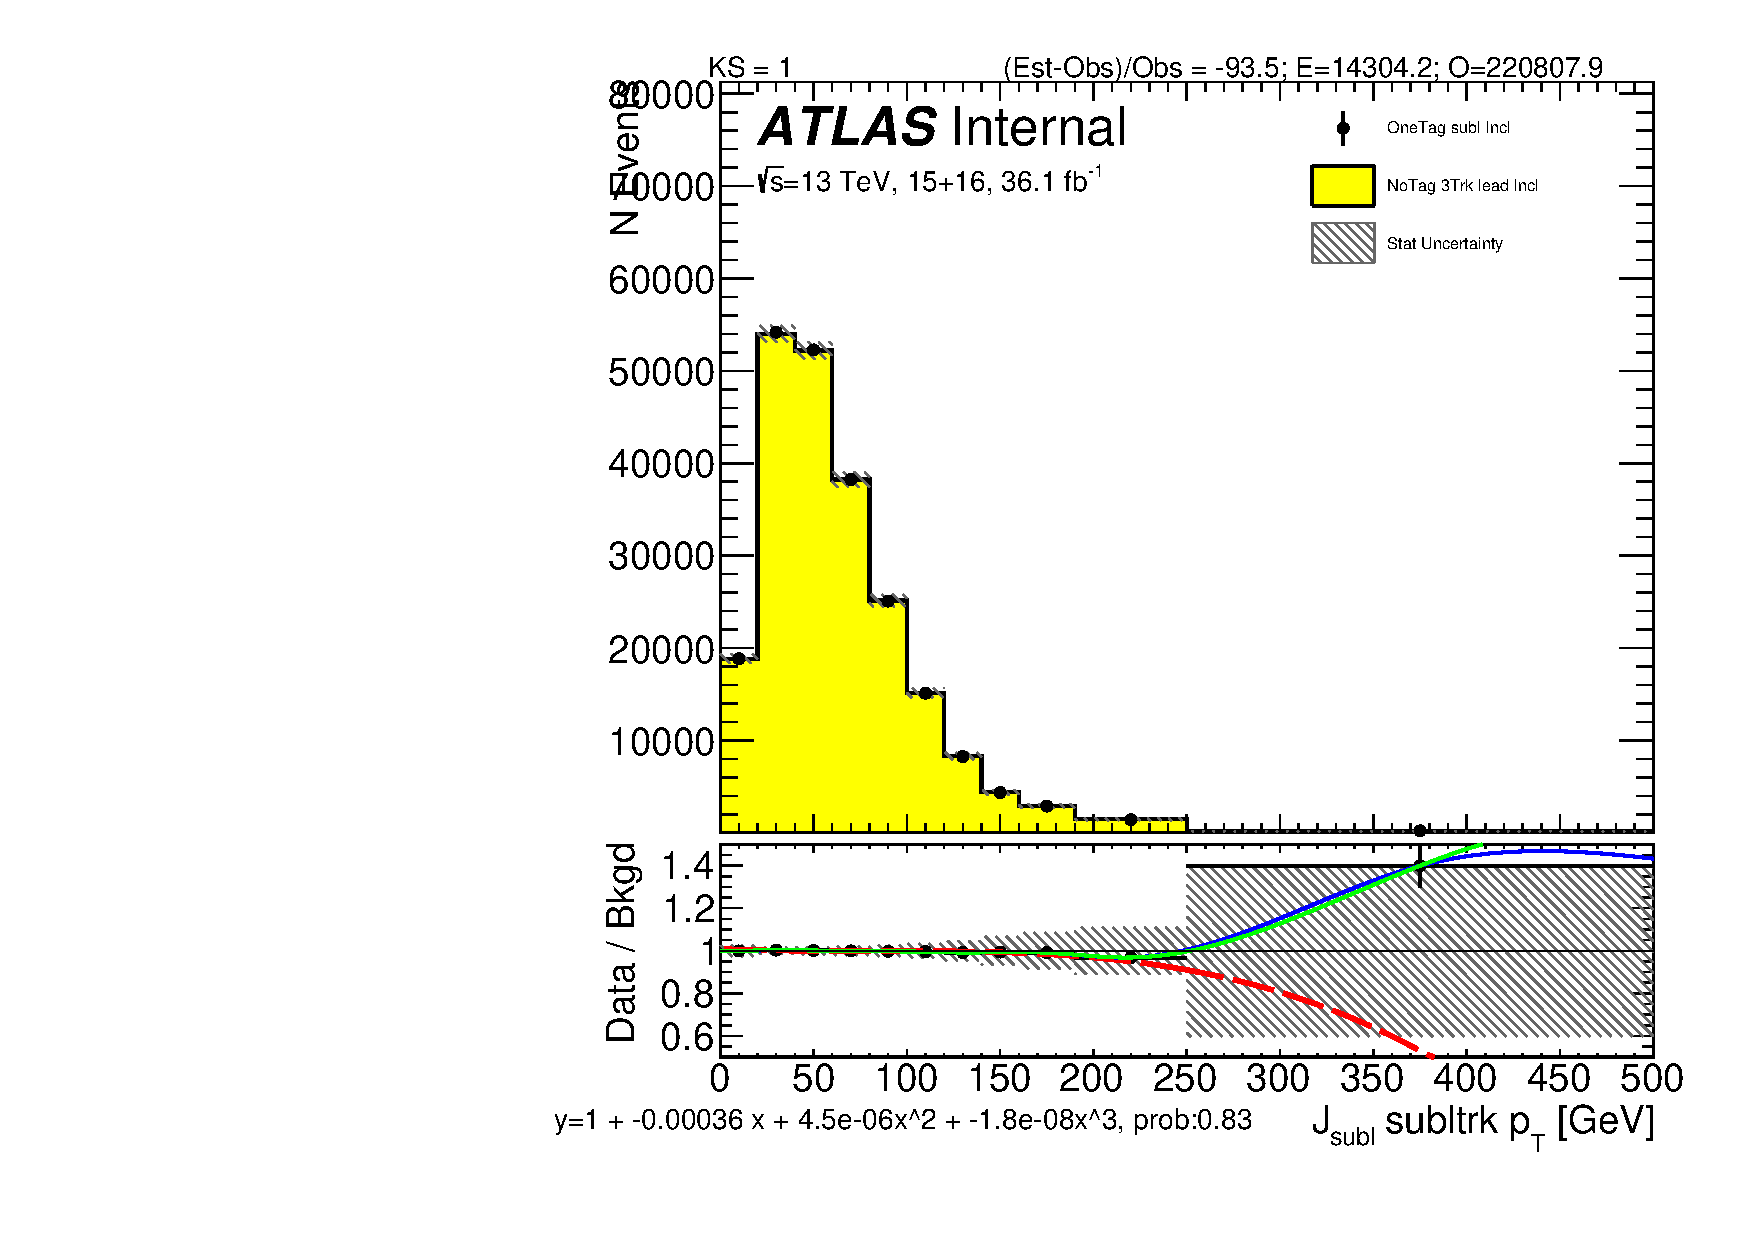
\includegraphics[width=0.25\textwidth,angle=-90]{figures/boosted/Reweight/Fits/Moriond_bkg_3_NoTag_3Trk_lead_Incl_sublHCand_trk1_Pt.pdf} \\
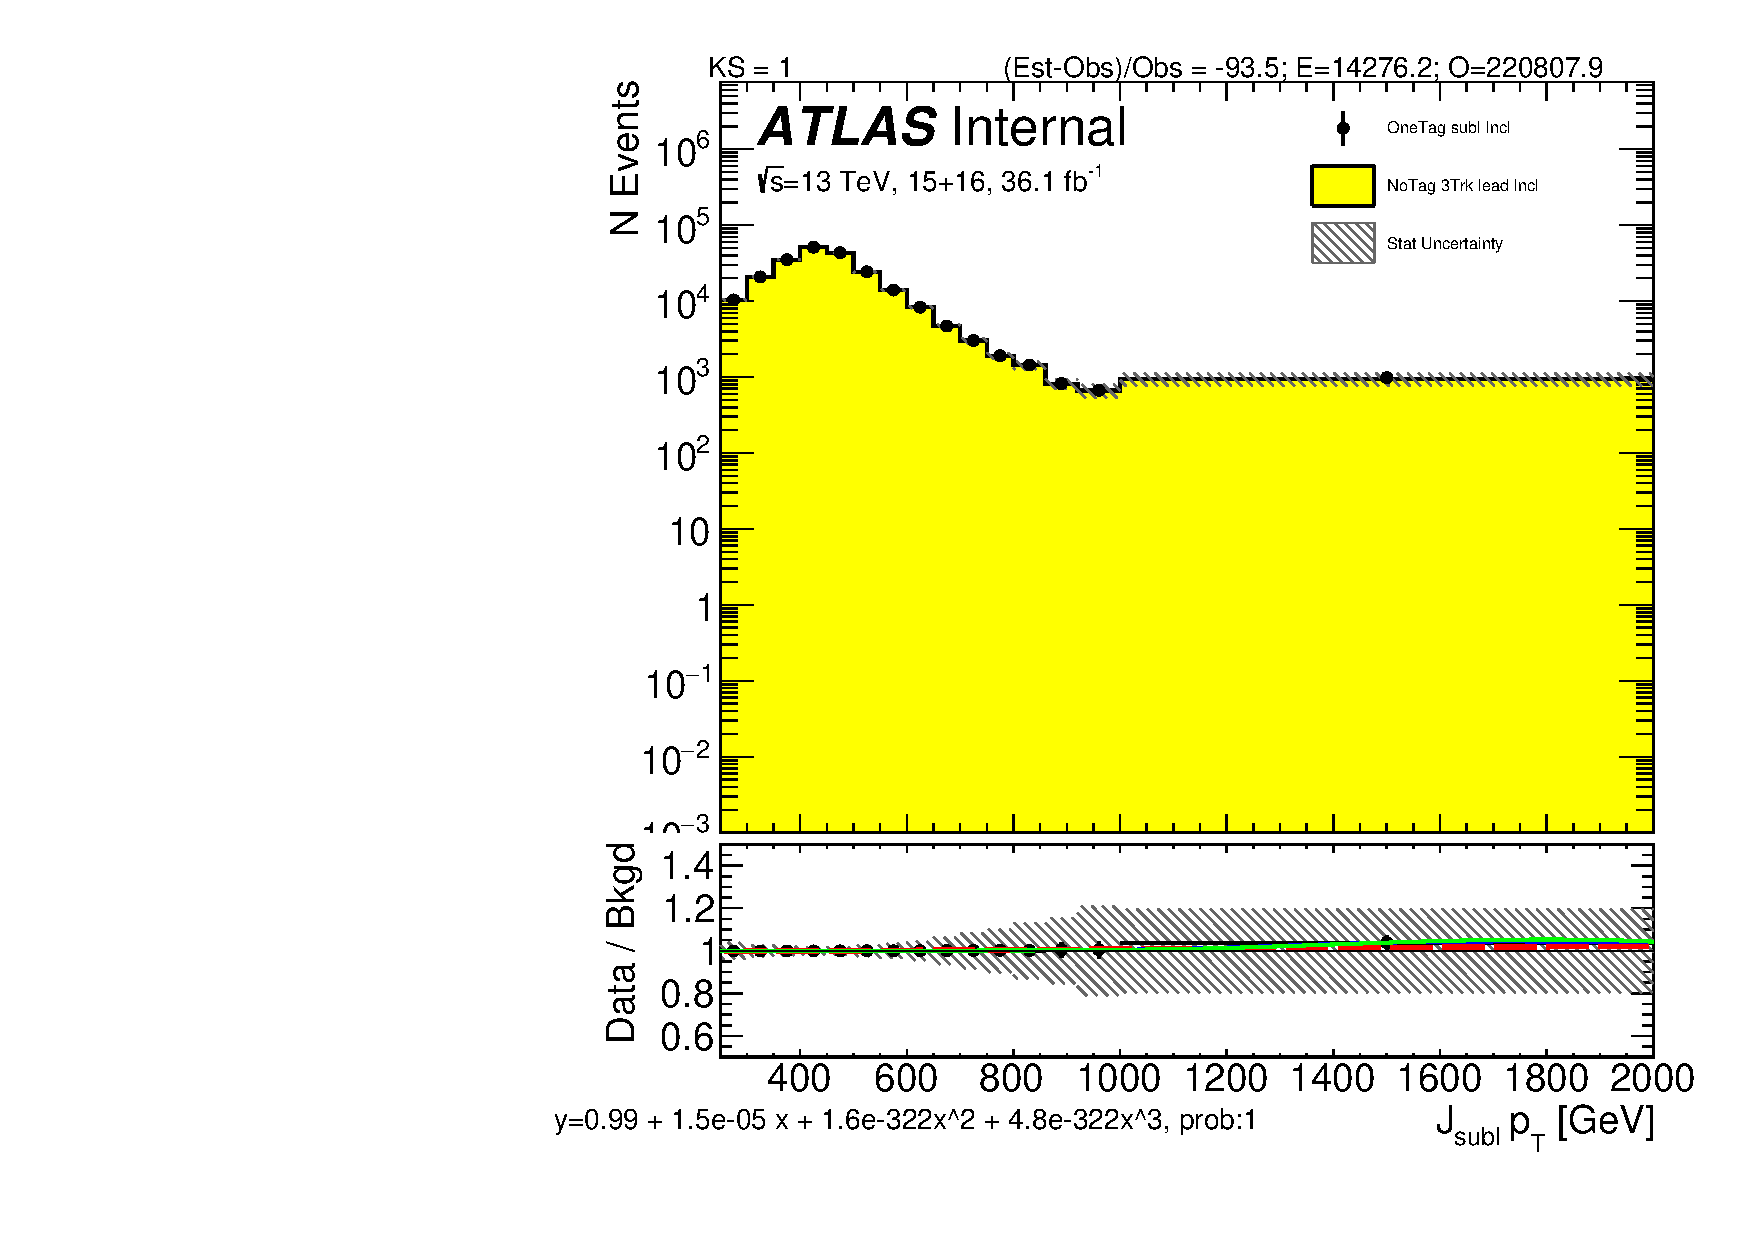
\includegraphics[width=0.25\textwidth,angle=-90]{figures/boosted/Reweight/Fits/Moriond_bkg_9_NoTag_3Trk_lead_Incl_sublHCand_Pt_m_1.pdf}
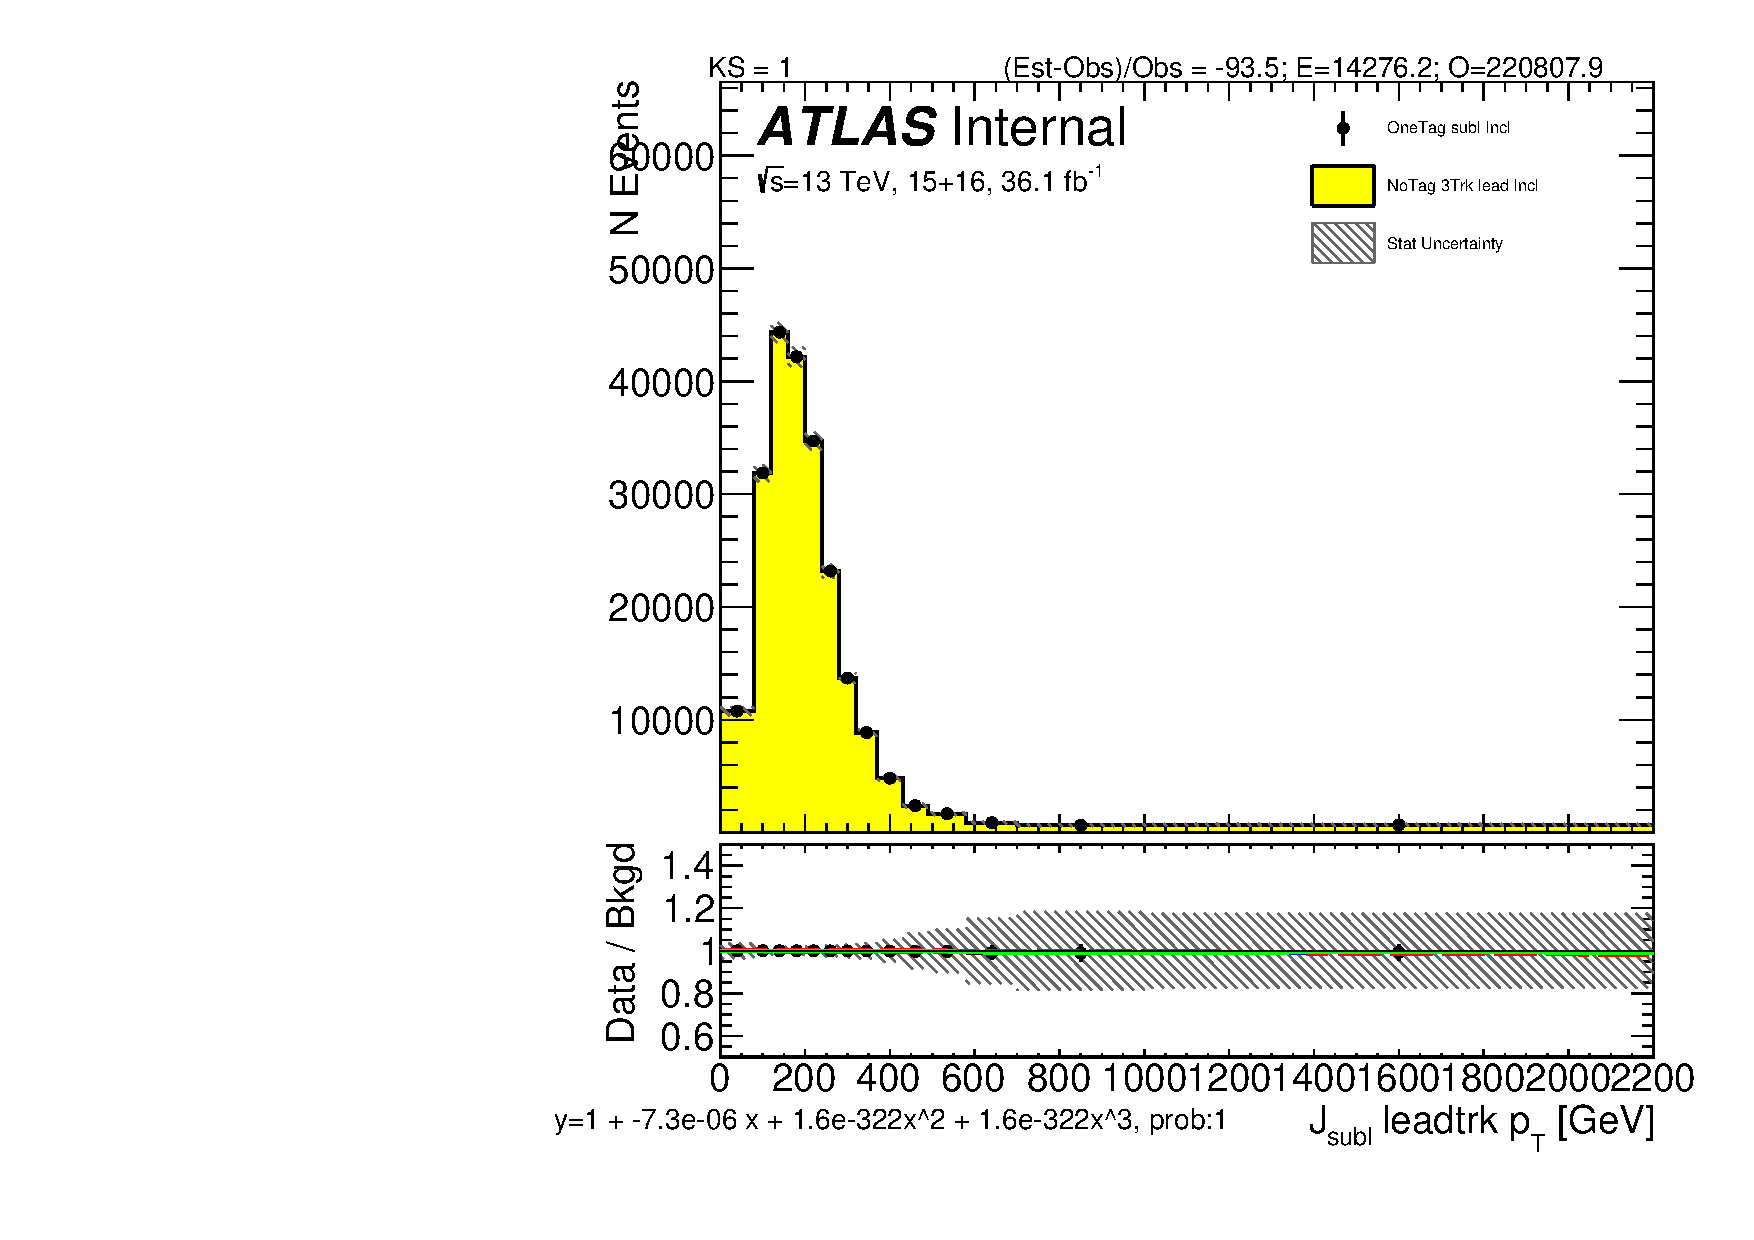
\includegraphics[width=0.25\textwidth,angle=-90]{figures/boosted/Reweight/Fits/Moriond_bkg_9_NoTag_3Trk_lead_Incl_sublHCand_trk0_Pt.pdf}
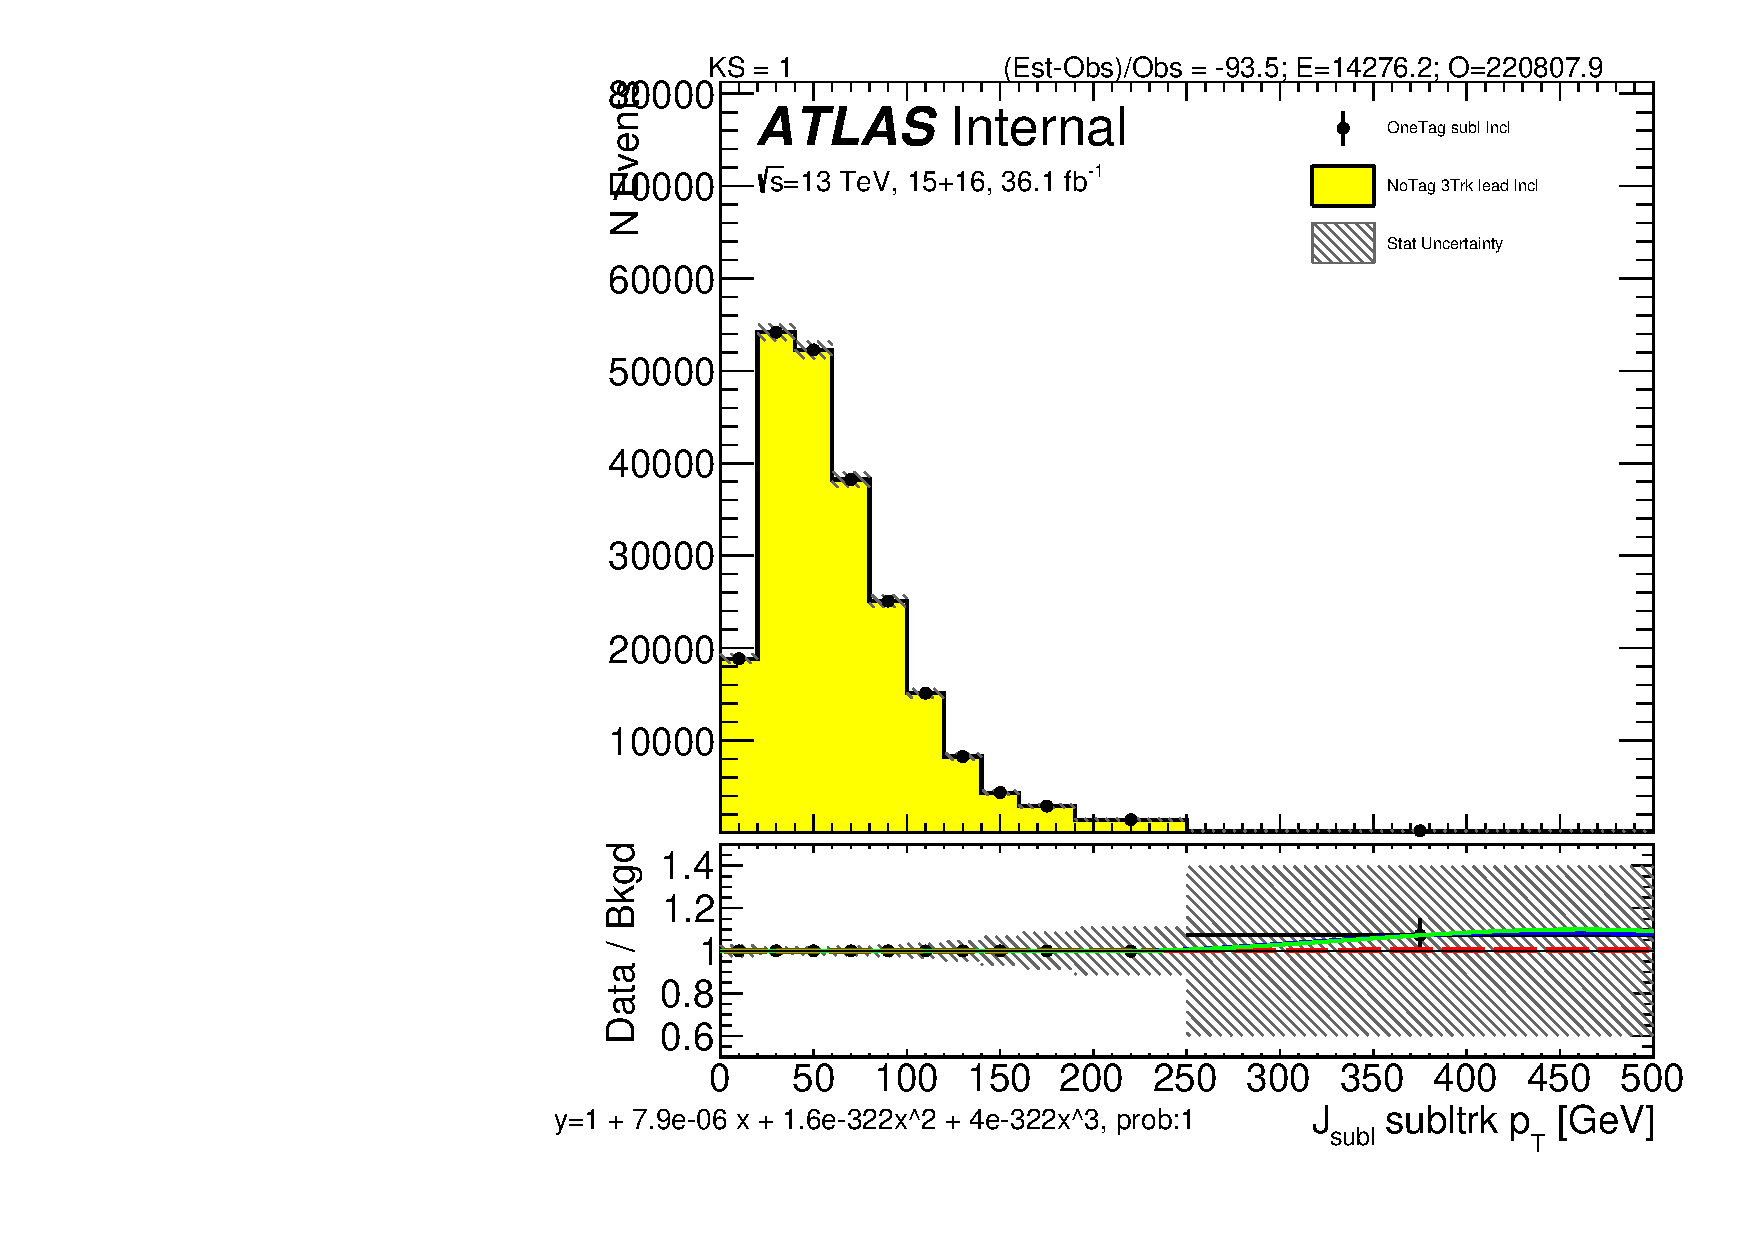
\includegraphics[width=0.25\textwidth,angle=-90]{figures/boosted/Reweight/Fits/Moriond_bkg_9_NoTag_3Trk_lead_Incl_sublHCand_trk1_Pt.pdf} \\
\caption{For $3b$ background estimate: the fits to the ratio of the data in the $2b$ category, of the subleading Higgs candidate $2b$-tagged events' subleading Higgs candidate distributions(black point), over the leading Higgs candidate $1b$-tagged events' subleading Higgs candidate distributions(yellow). Distributions and fits to the estimated QCD background for large-\R jet $p_{T}$ (left),  the large-\R jet's leading track jet $p_T$ (middle), and large-\R jet's subleading track jet $p_T$ (right) are shown.  Figures are before reweighting (top row), after the first iteration(second row), after the fourth iteration(third row), and after the last iteration (bottom row). The green line is the spline fit; the red line is a polynomial fit; the blue line is the spline interpolation.}
\label{fig:rw-3b-lead}
\end{center}
\end{figure*}

\begin{figure*}[htbp!]
\begin{center}
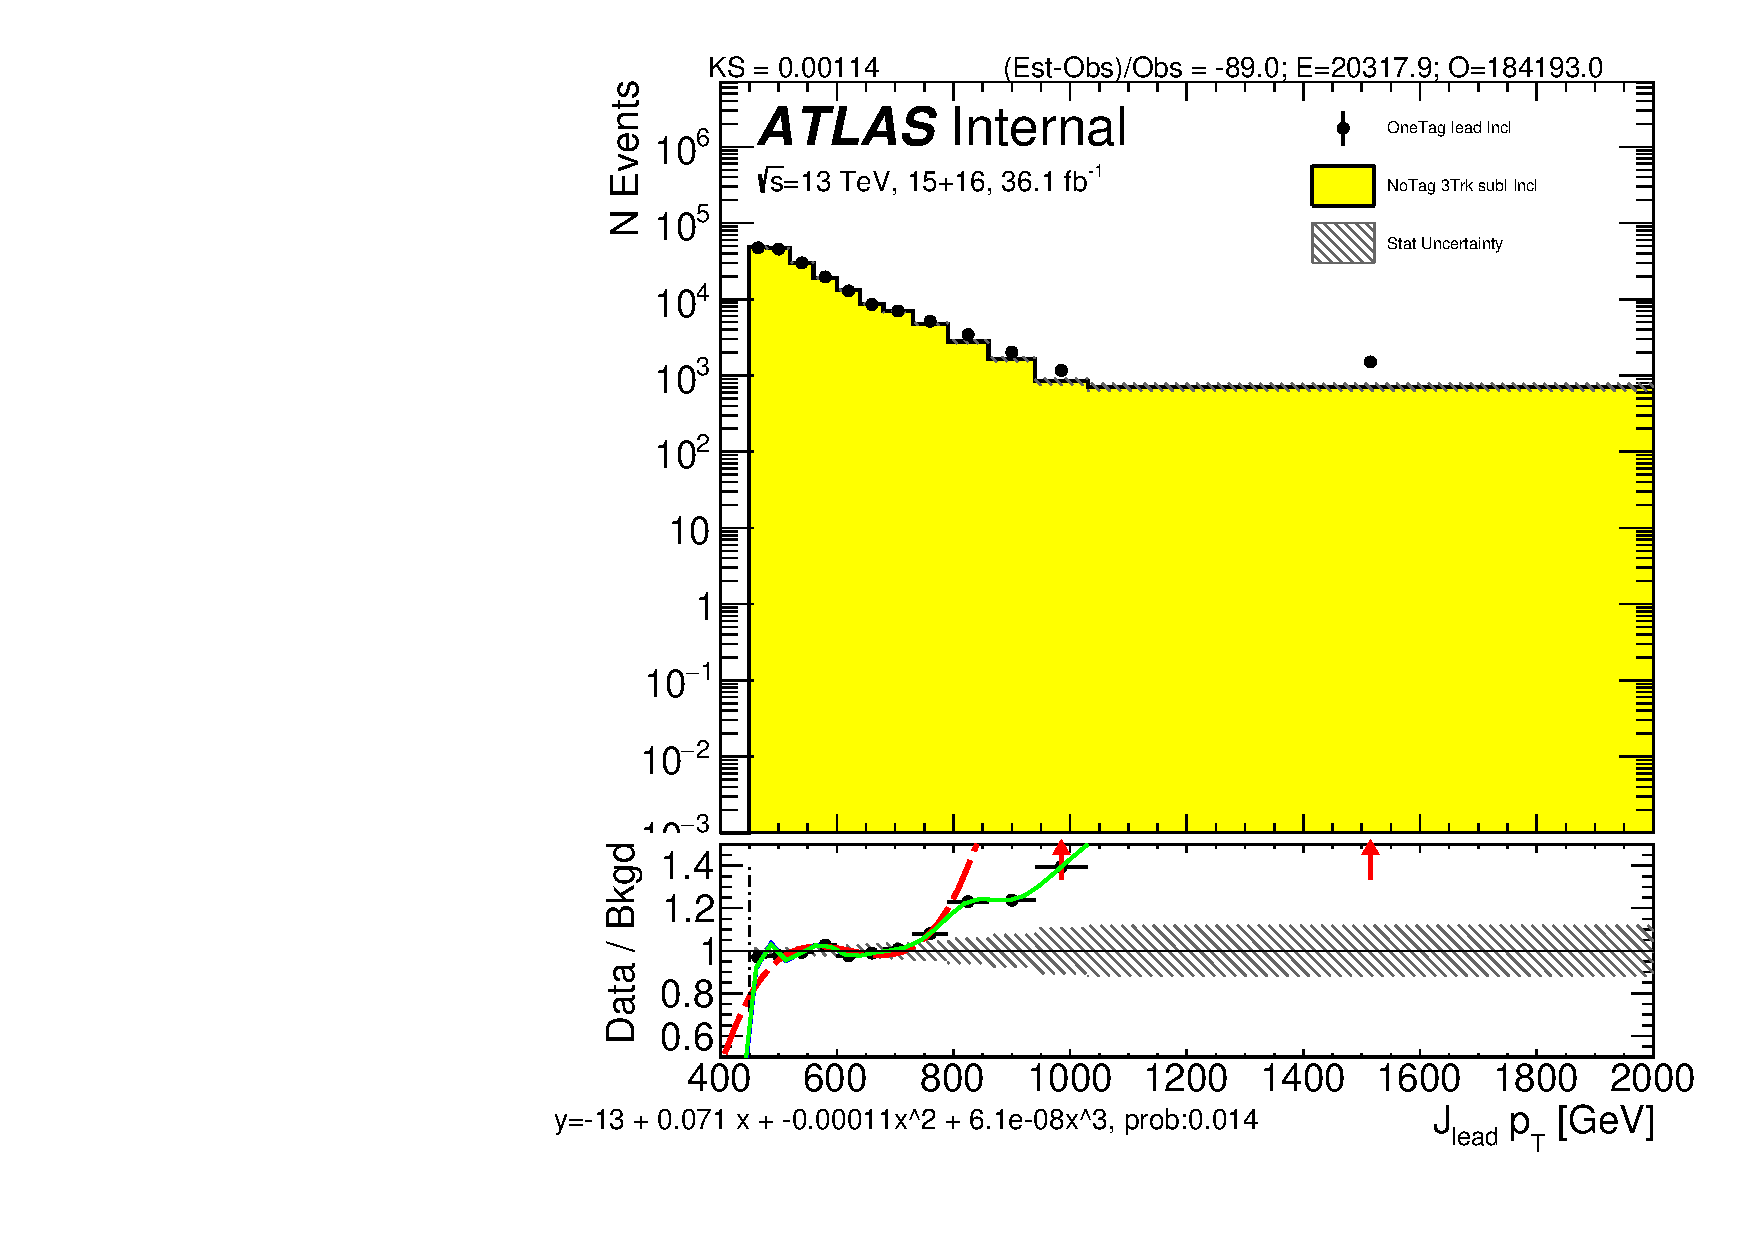
\includegraphics[width=0.25\textwidth,angle=-90]{figures/boosted/Reweight/Fits/Moriond_NoTag_3Trk_subl_Incl_leadHCand_Pt_m_1.pdf}
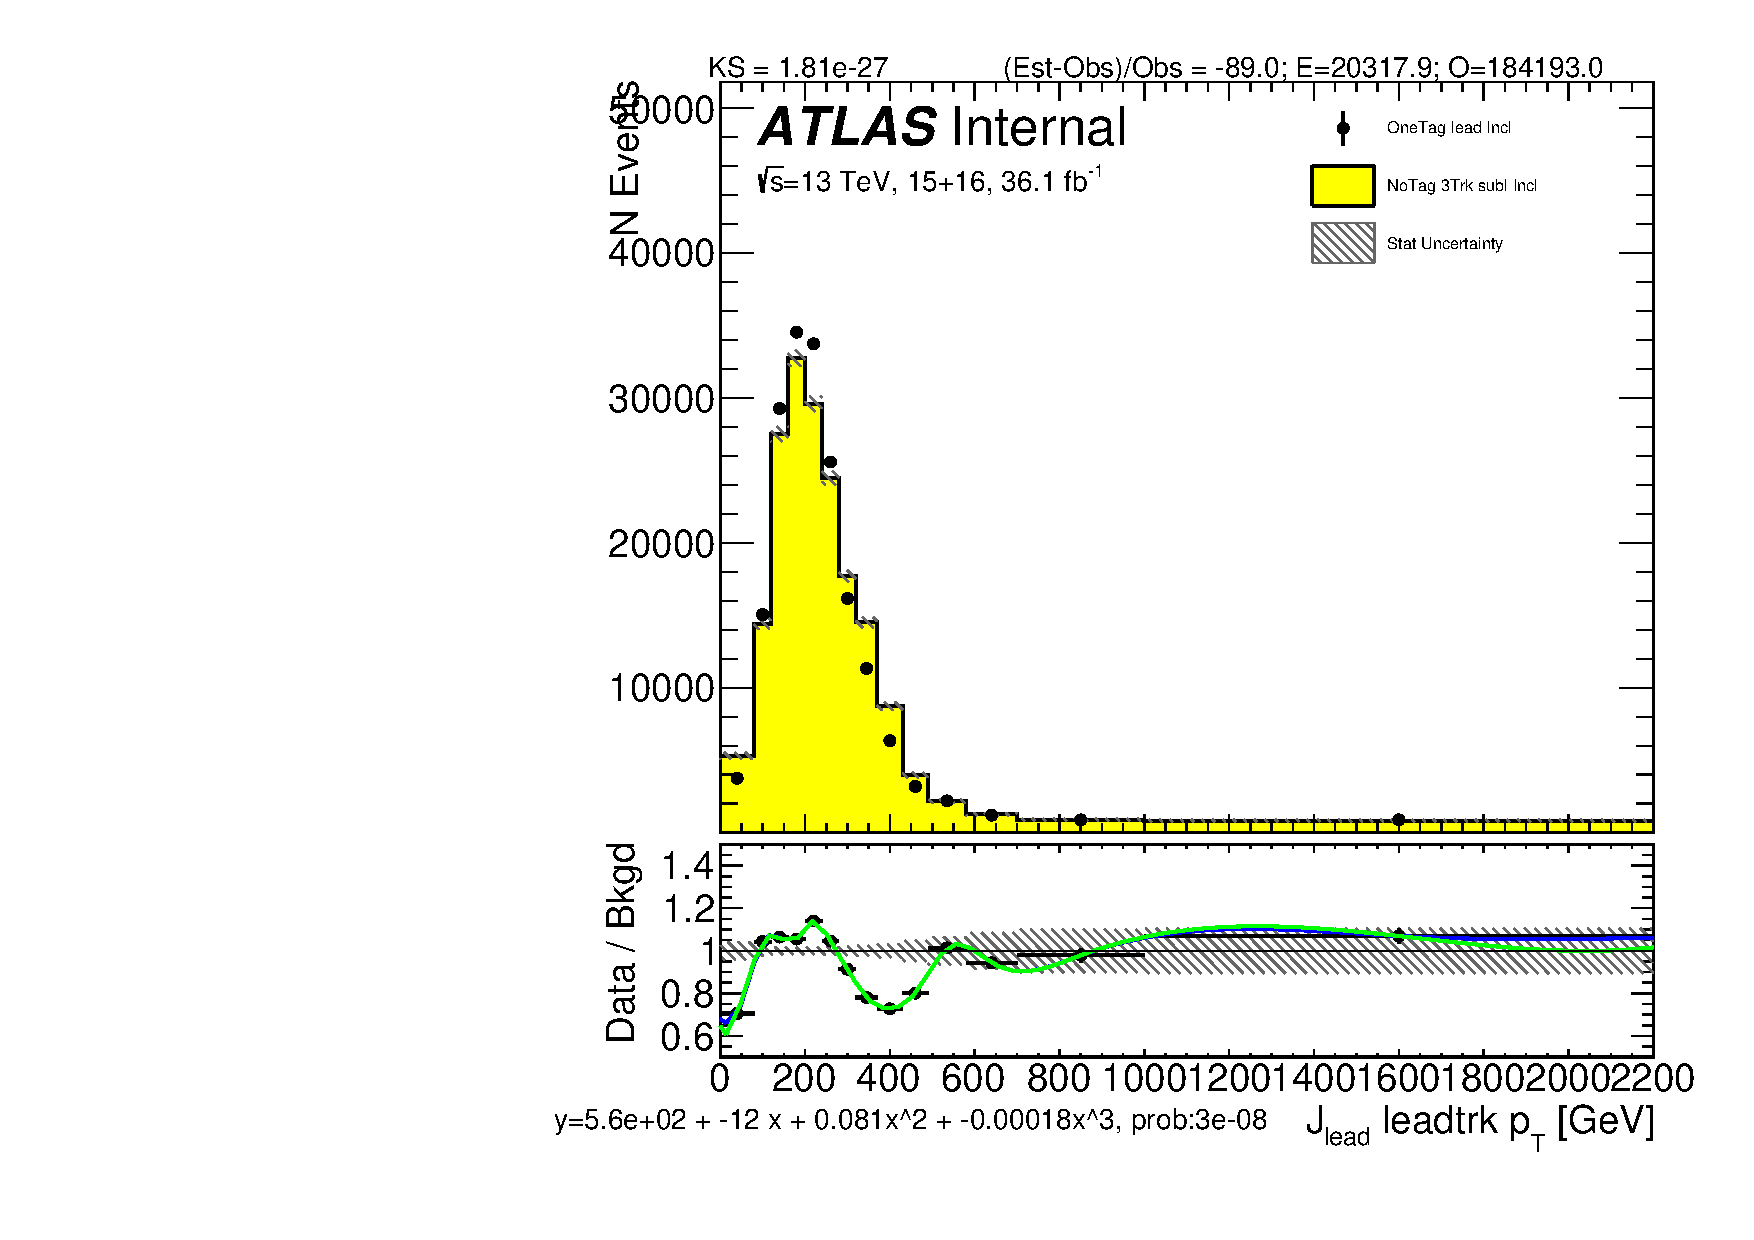
\includegraphics[width=0.25\textwidth,angle=-90]{figures/boosted/Reweight/Fits/Moriond_NoTag_3Trk_subl_Incl_leadHCand_trk0_Pt.pdf}
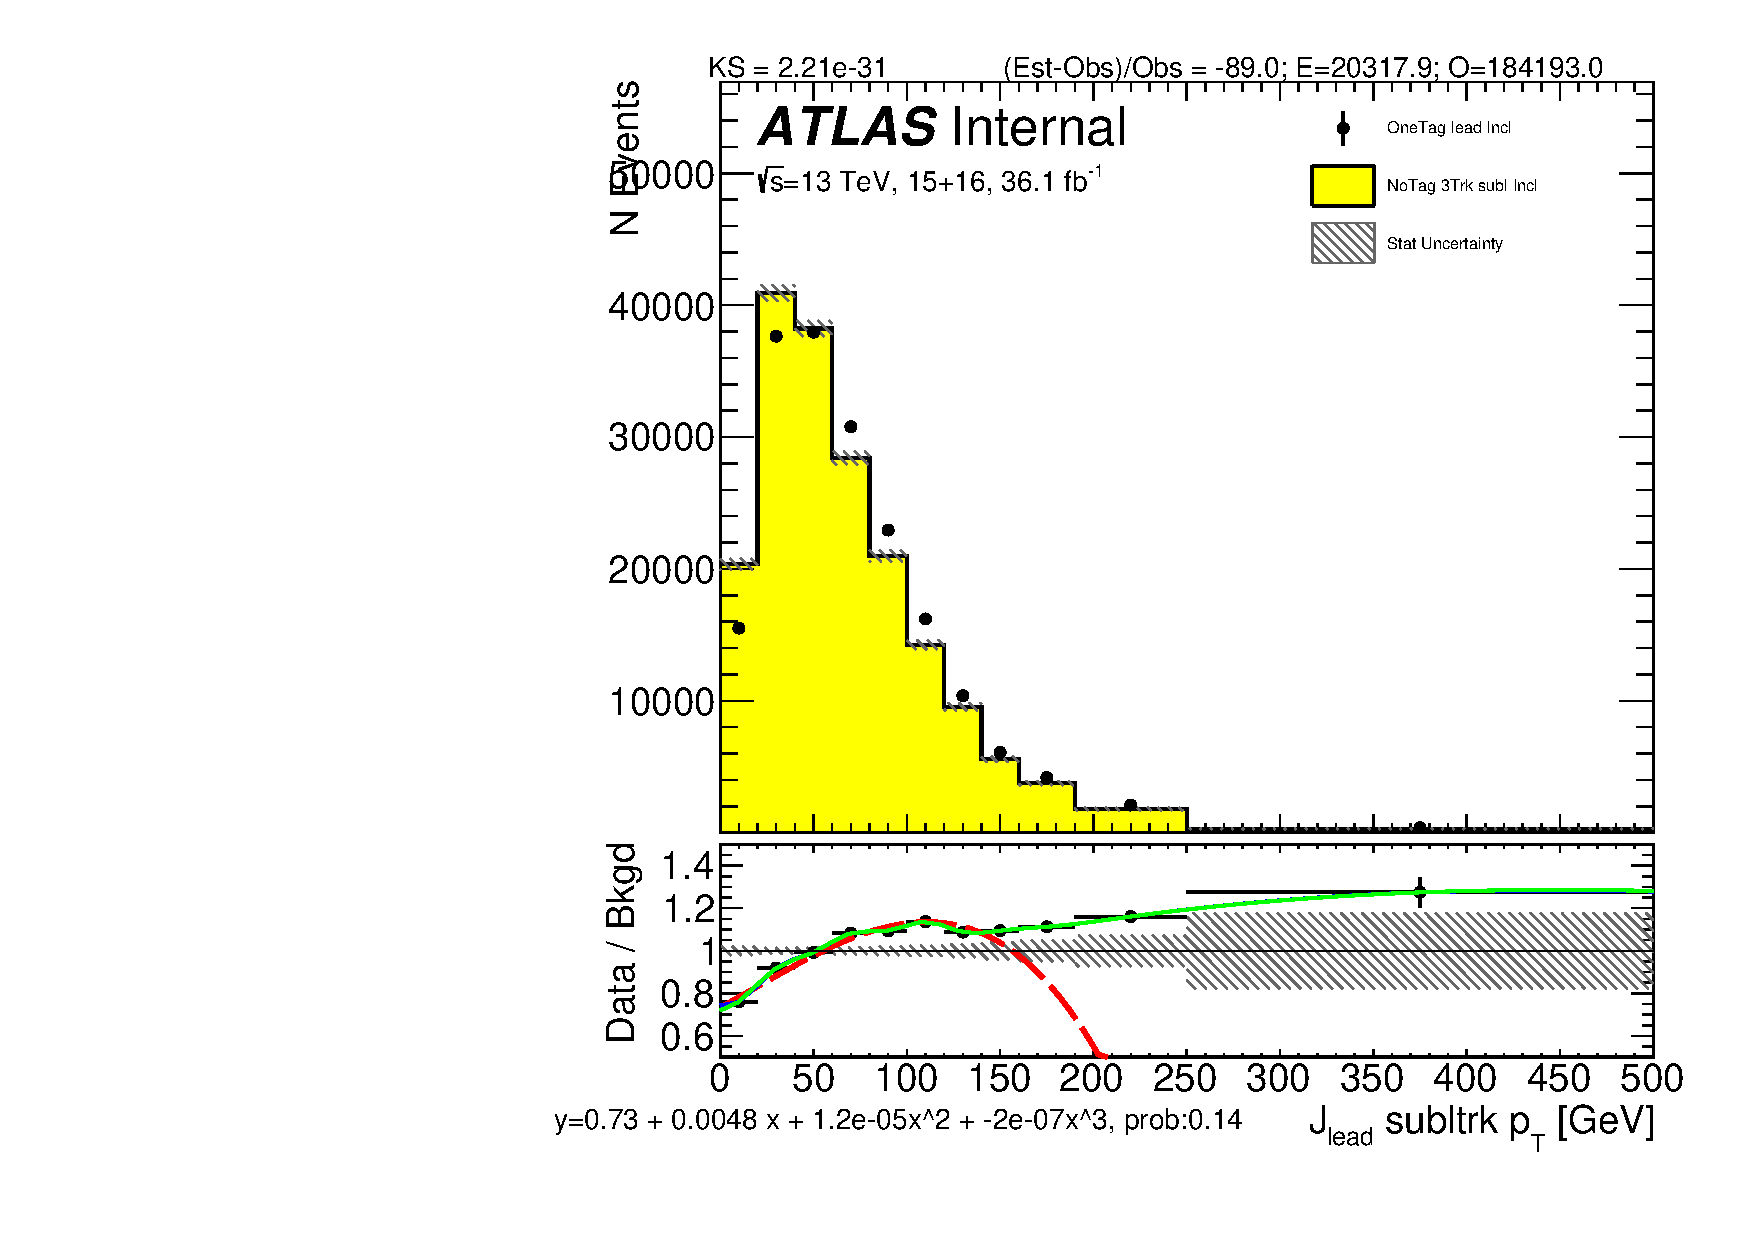
\includegraphics[width=0.25\textwidth,angle=-90]{figures/boosted/Reweight/Fits/Moriond_NoTag_3Trk_subl_Incl_leadHCand_trk1_Pt.pdf} \\
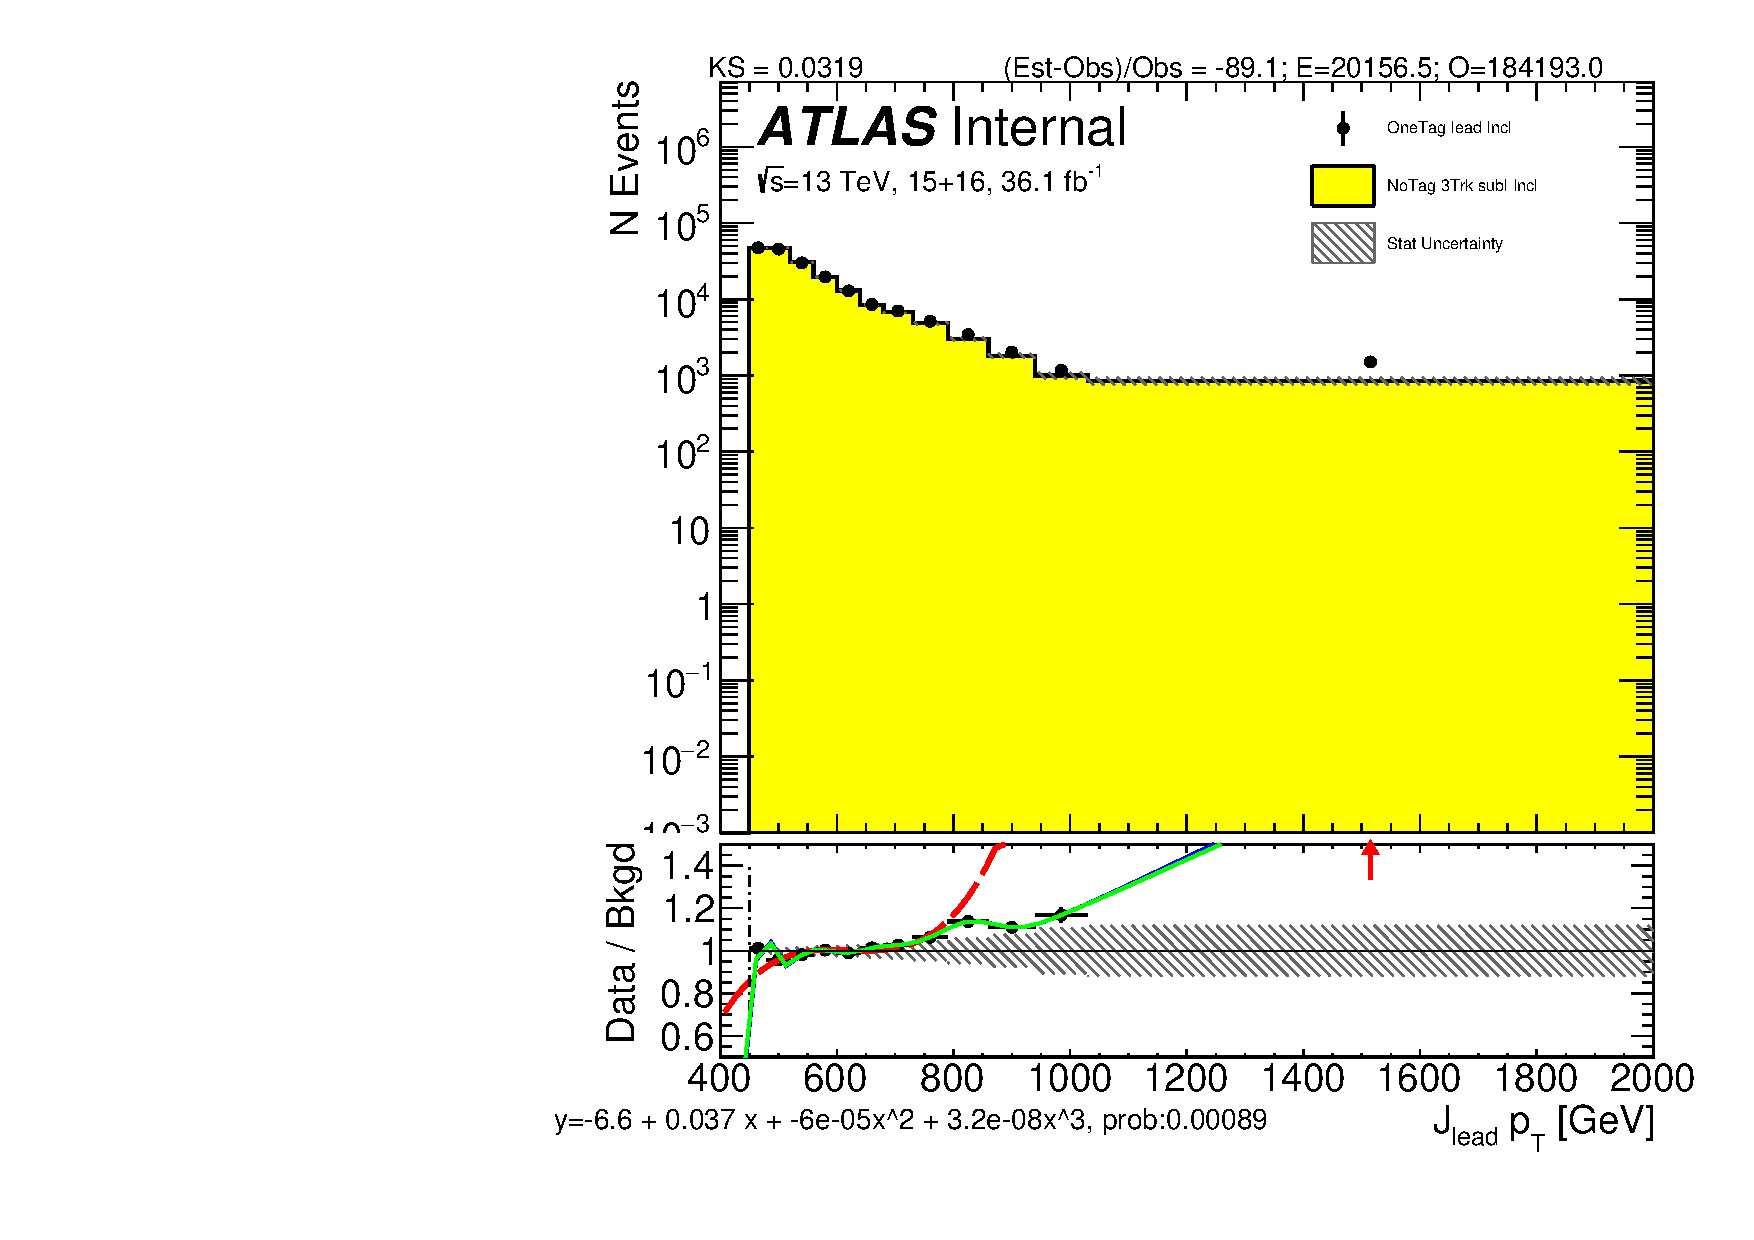
\includegraphics[width=0.25\textwidth,angle=-90]{figures/boosted/Reweight/Fits/Moriond_bkg_0_NoTag_3Trk_subl_Incl_leadHCand_Pt_m_1.pdf}
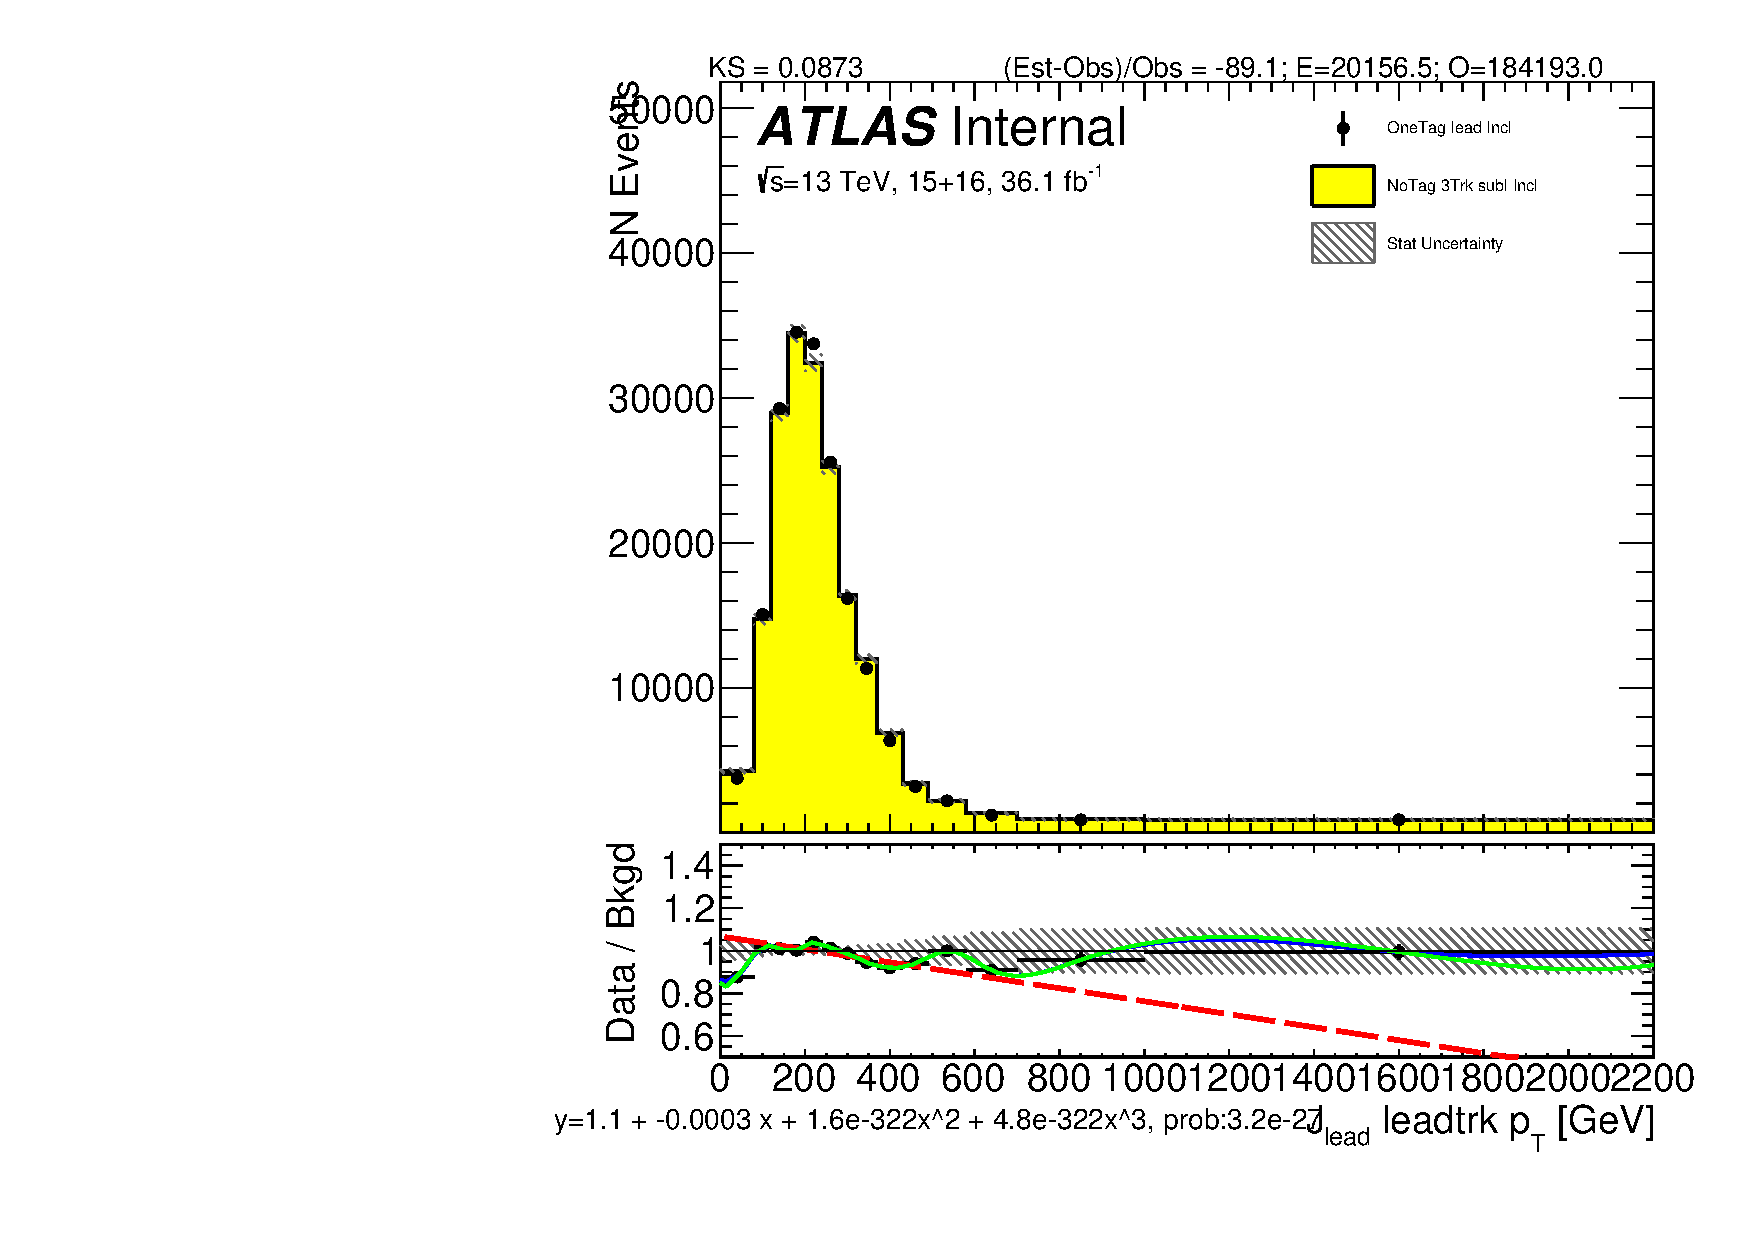
\includegraphics[width=0.25\textwidth,angle=-90]{figures/boosted/Reweight/Fits/Moriond_bkg_0_NoTag_3Trk_subl_Incl_leadHCand_trk0_Pt.pdf}
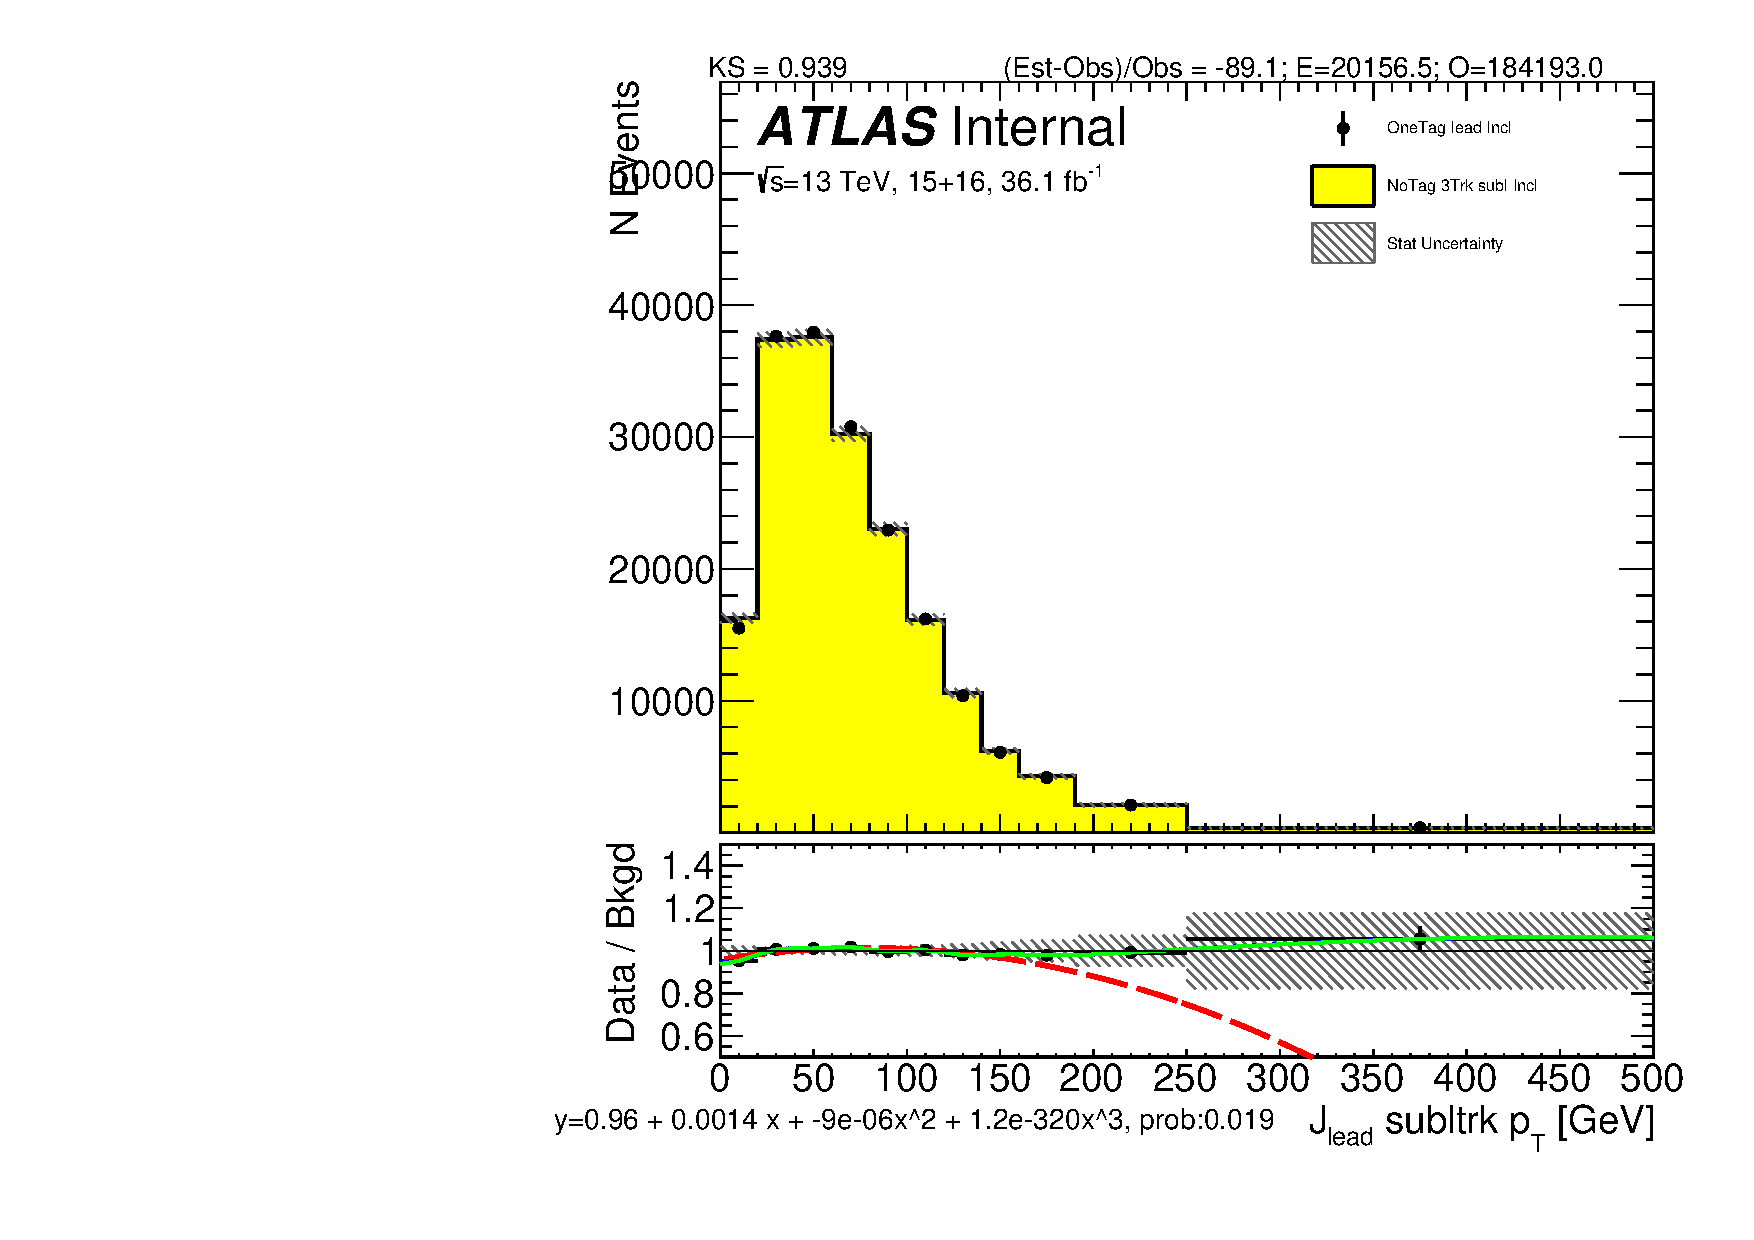
\includegraphics[width=0.25\textwidth,angle=-90]{figures/boosted/Reweight/Fits/Moriond_bkg_0_NoTag_3Trk_subl_Incl_leadHCand_trk1_Pt.pdf} \\
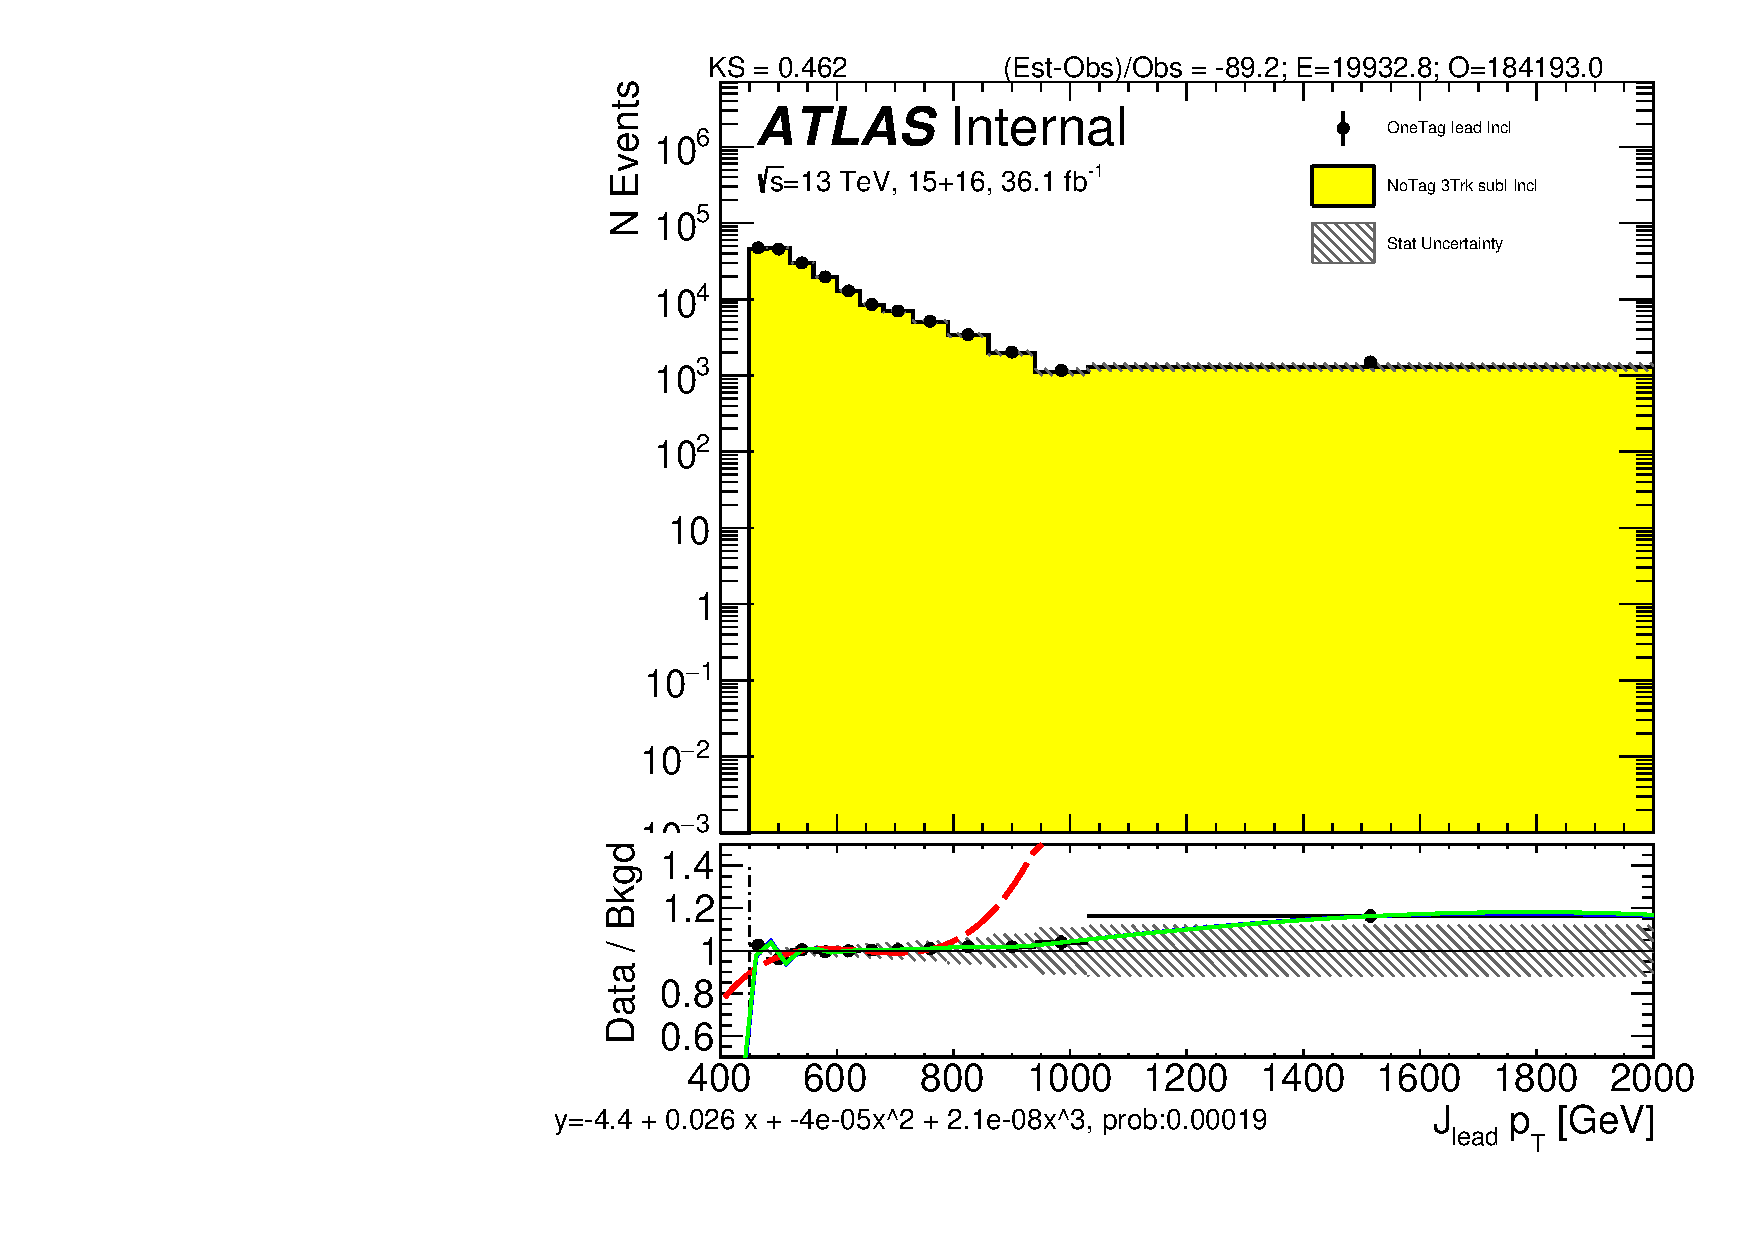
\includegraphics[width=0.25\textwidth,angle=-90]{figures/boosted/Reweight/Fits/Moriond_bkg_3_NoTag_3Trk_subl_Incl_leadHCand_Pt_m_1.pdf}
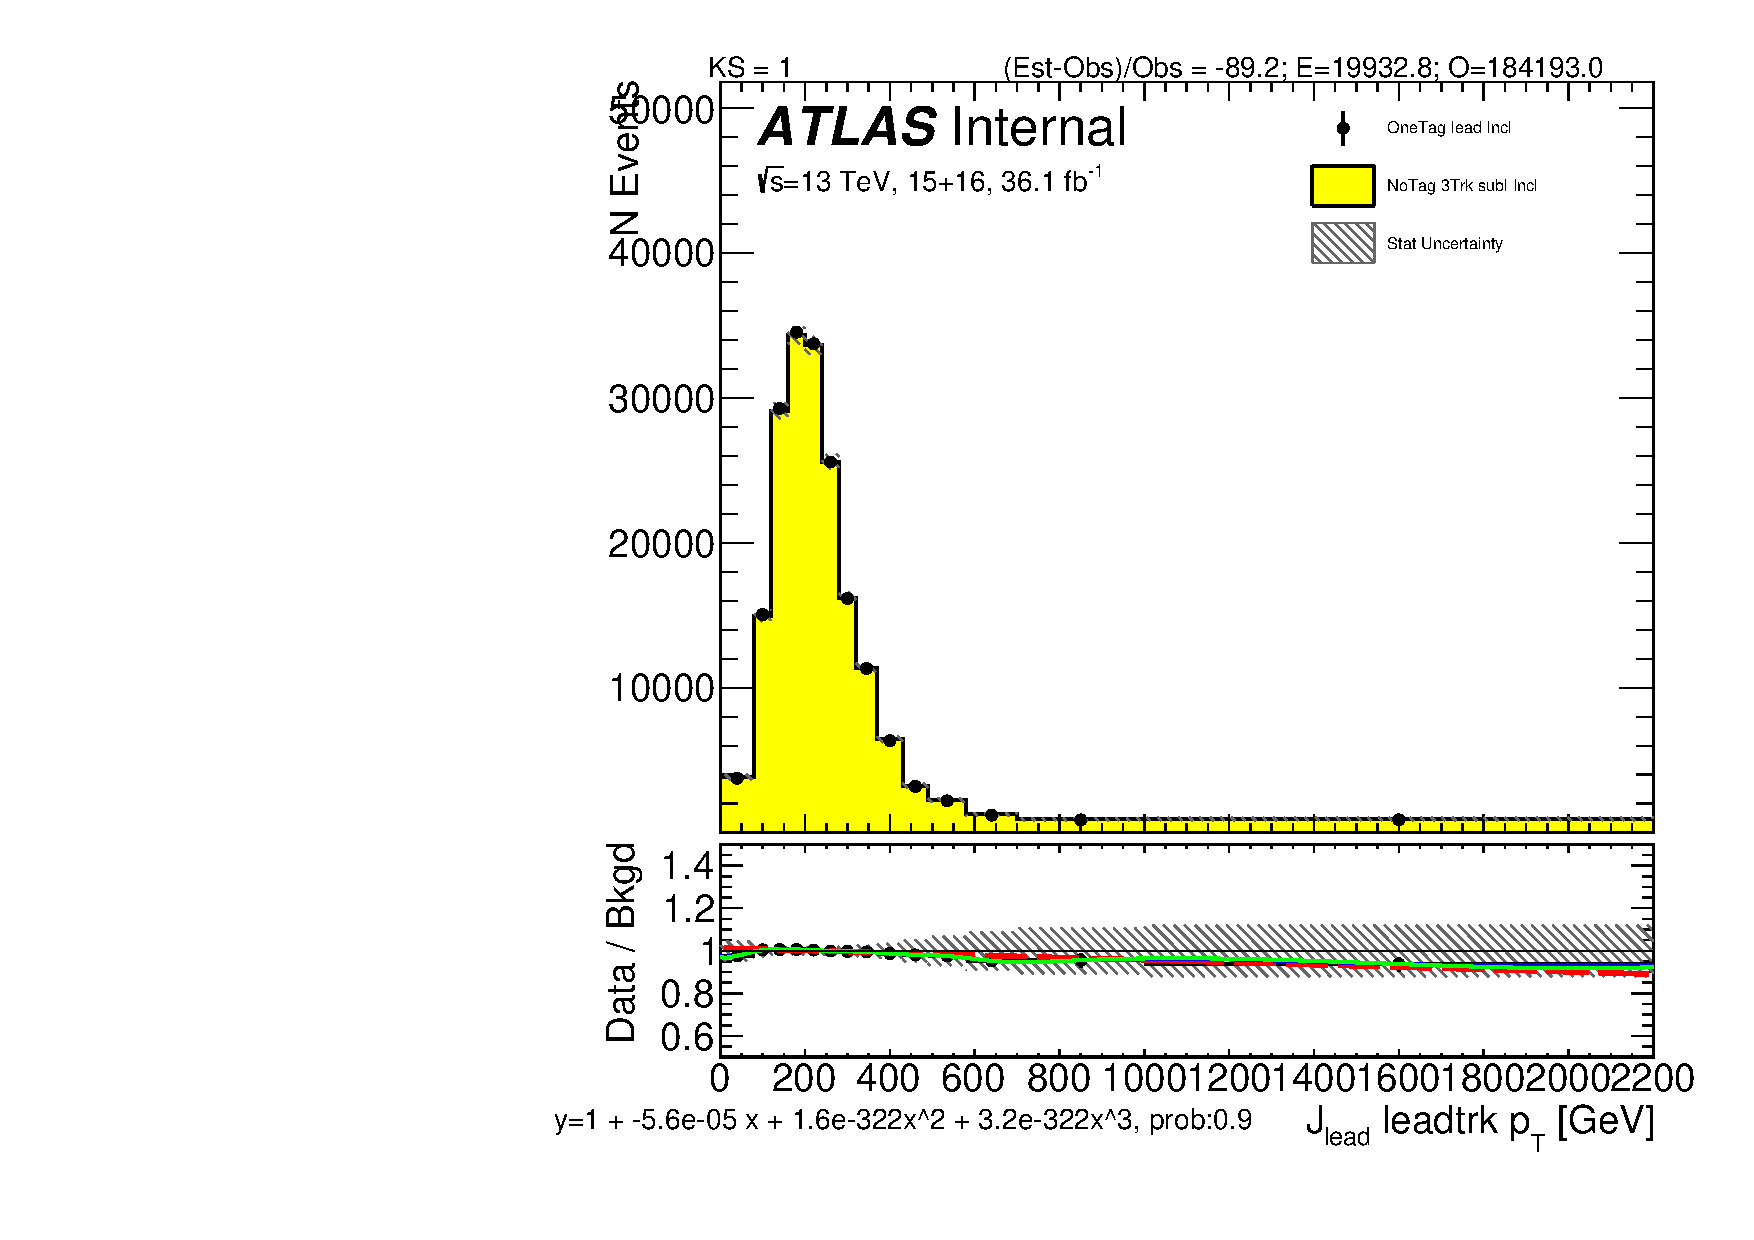
\includegraphics[width=0.25\textwidth,angle=-90]{figures/boosted/Reweight/Fits/Moriond_bkg_3_NoTag_3Trk_subl_Incl_leadHCand_trk0_Pt.pdf}
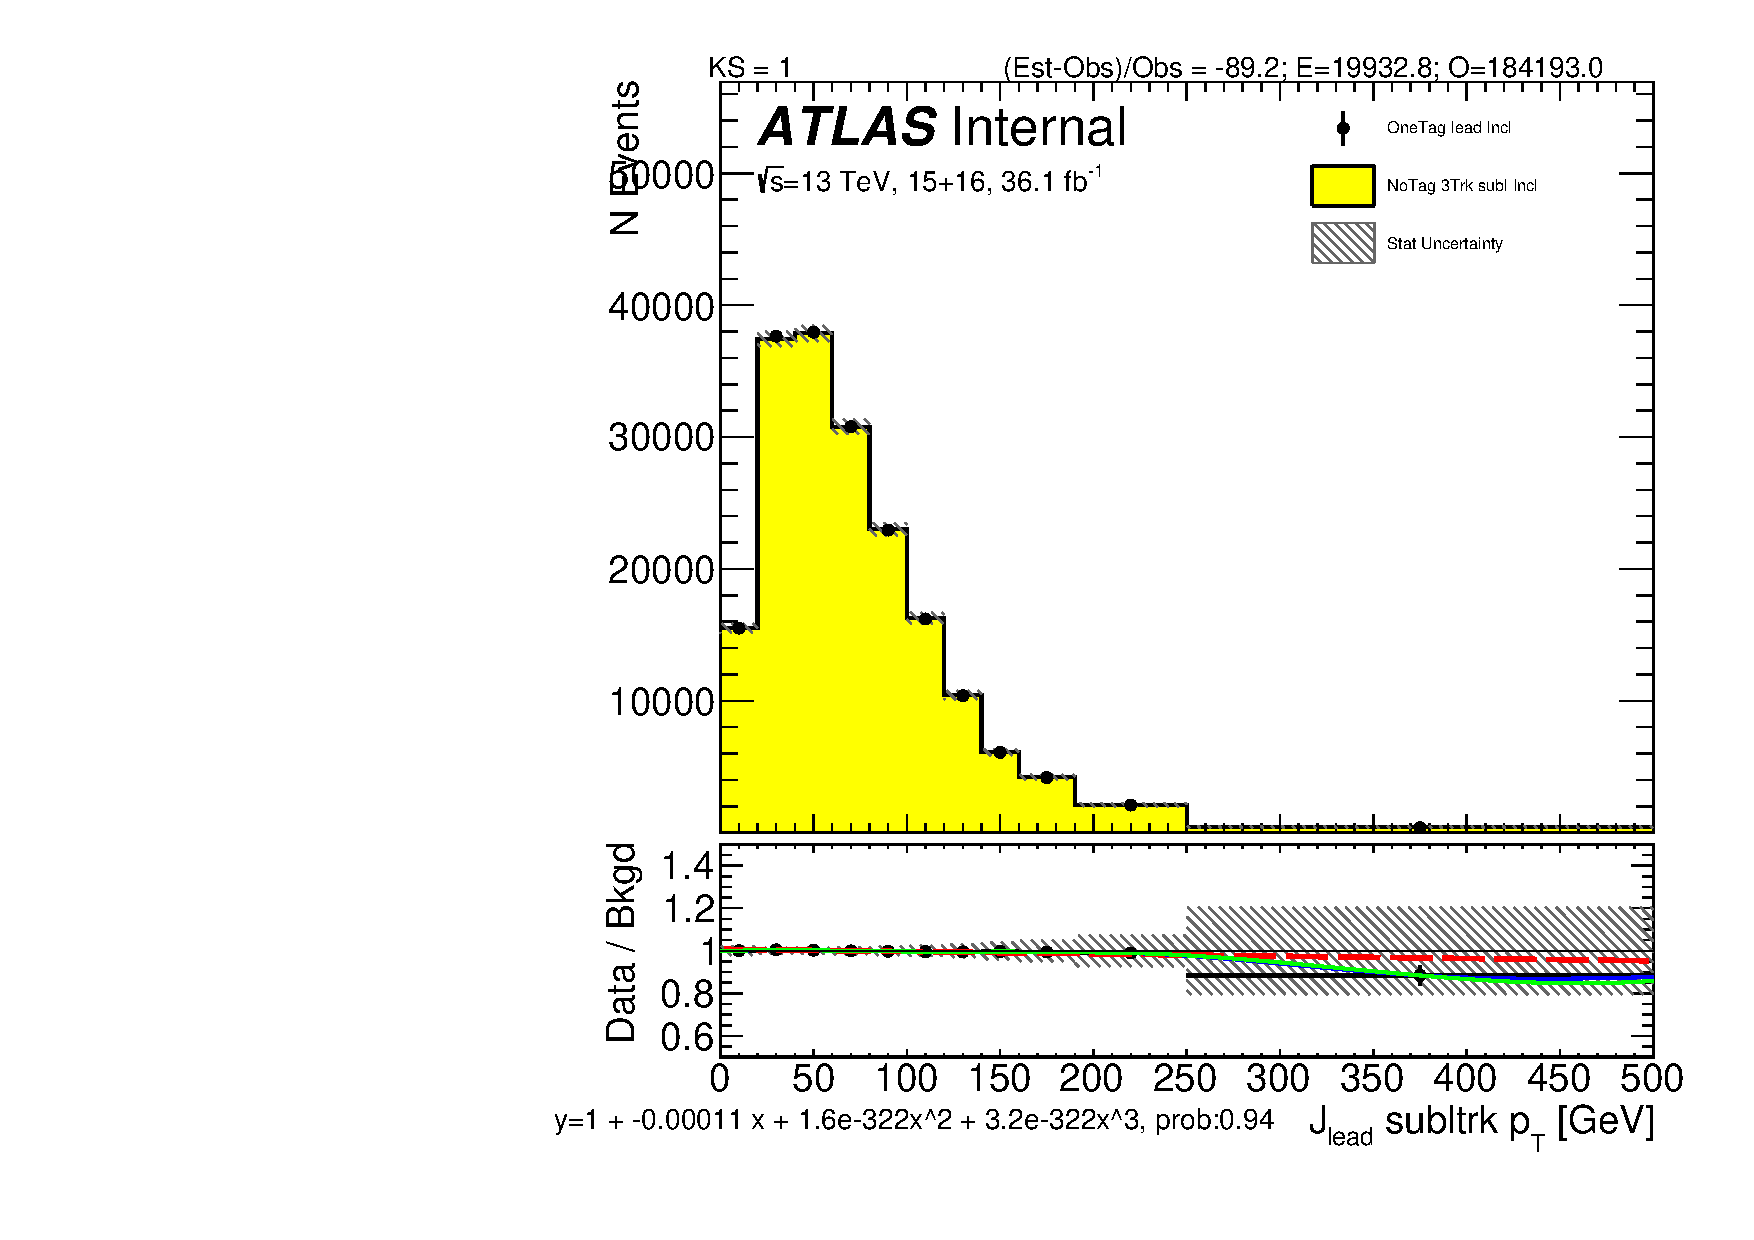
\includegraphics[width=0.25\textwidth,angle=-90]{figures/boosted/Reweight/Fits/Moriond_bkg_3_NoTag_3Trk_subl_Incl_leadHCand_trk1_Pt.pdf} \\
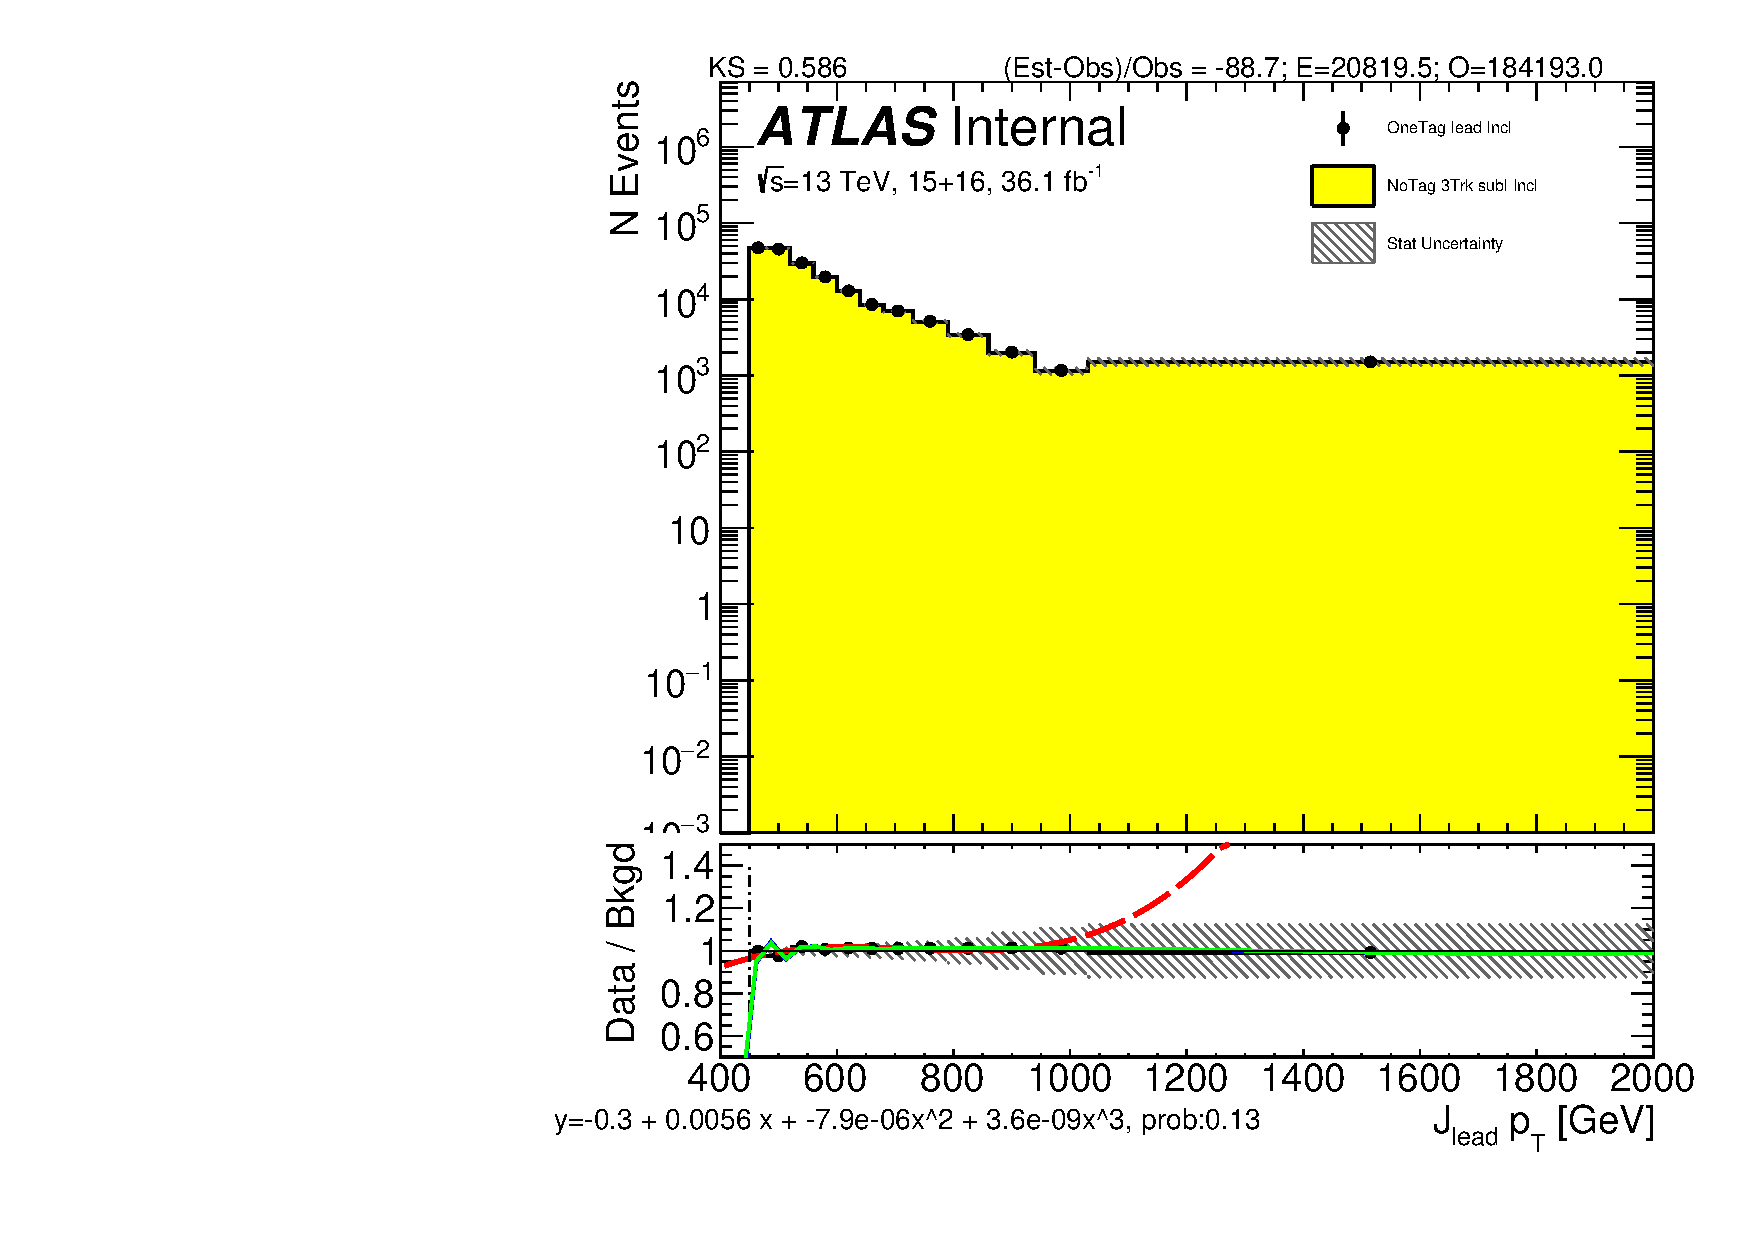
\includegraphics[width=0.25\textwidth,angle=-90]{figures/boosted/Reweight/Fits/Moriond_bkg_9_NoTag_3Trk_subl_Incl_leadHCand_Pt_m_1.pdf}
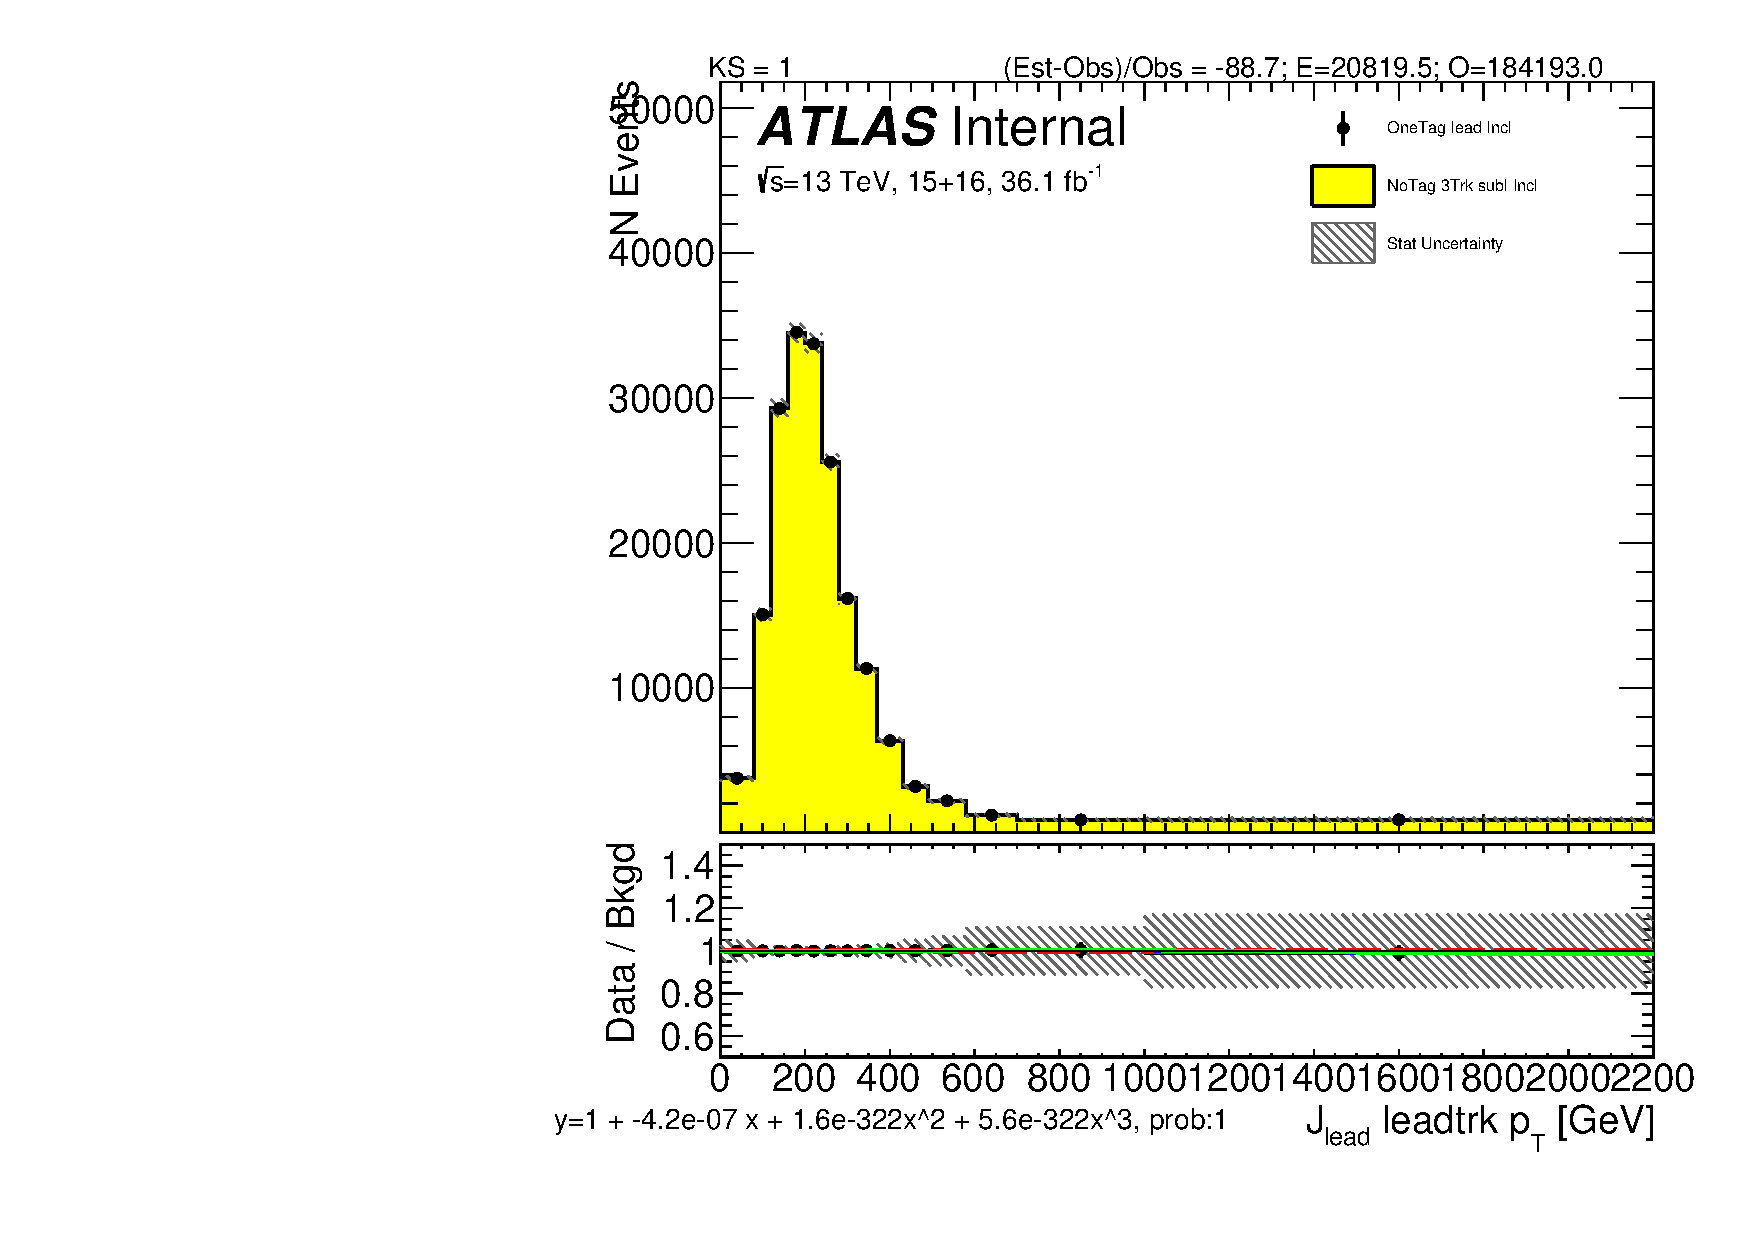
\includegraphics[width=0.25\textwidth,angle=-90]{figures/boosted/Reweight/Fits/Moriond_bkg_9_NoTag_3Trk_subl_Incl_leadHCand_trk0_Pt.pdf}
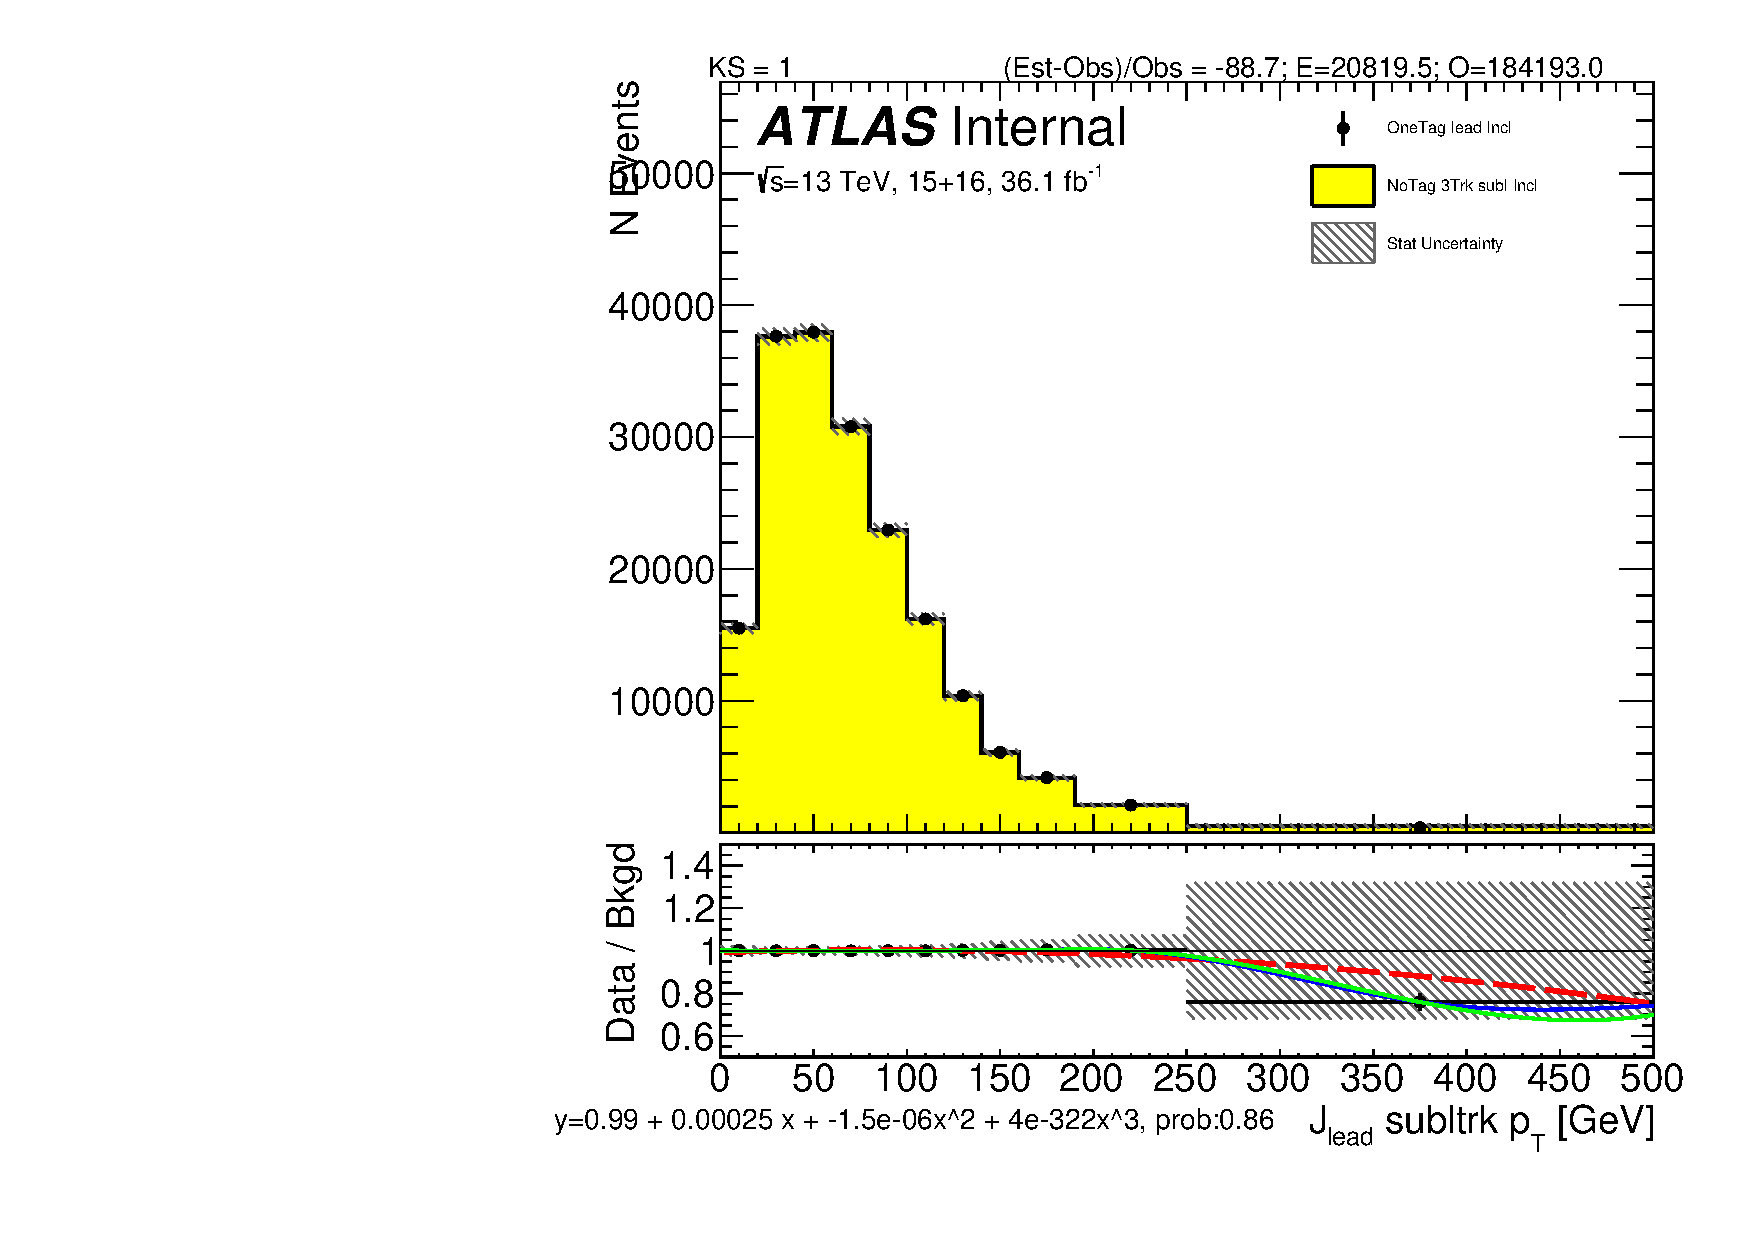
\includegraphics[width=0.25\textwidth,angle=-90]{figures/boosted/Reweight/Fits/Moriond_bkg_9_NoTag_3Trk_subl_Incl_leadHCand_trk1_Pt.pdf} \\
\caption{For $3b$ background estimate: the fits to the ratio of the data in the $2b$ category, of the leading Higgs candidate $2b$-tagged events' leading Higgs candidate distributions(black point), over the subleading Higgs candidate $1b$-tagged events' leading Higgs candidate distributions(yellow). Distributions and fits to the estimated QCD background for large-\R jet $p_{T}$ (left),  the large-\R jet's leading track jet $p_T$ (middle), and large-\R jet's subleading track jet $p_T$ (right) are shown.  Figures are before reweighting (top row), after the first iteration(second row), after the fourth iteration(third row), and after the last iteration (bottom row). The green line is the spline fit; the red line is a polynomial fit; the blue line is the spline interpolation.}
\label{fig:rw-3b-subl}
\end{center}
\end{figure*}

\begin{figure*}[htbp!]
\begin{center}
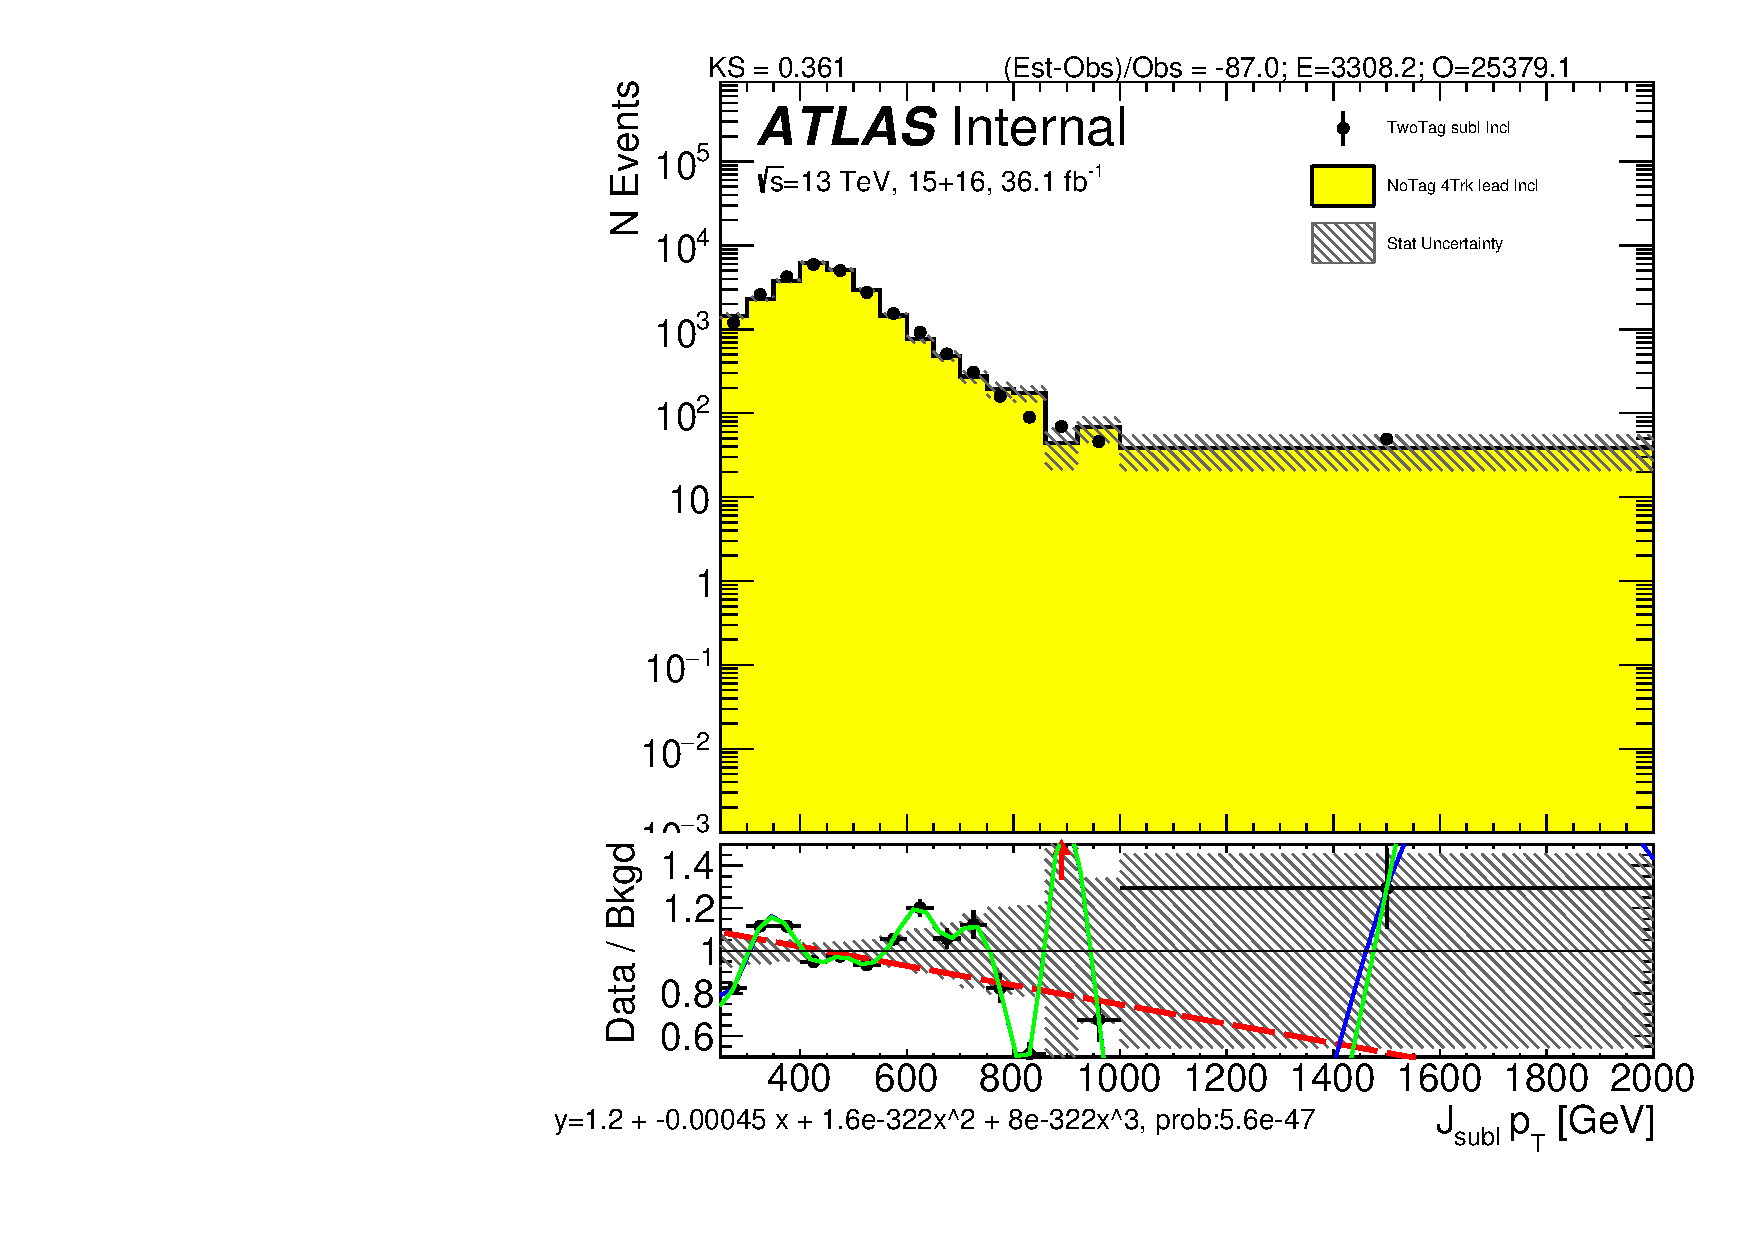
\includegraphics[width=0.25\textwidth,angle=-90]{figures/boosted/Reweight/Fits/Moriond_NoTag_4Trk_lead_Incl_sublHCand_Pt_m_1.pdf}
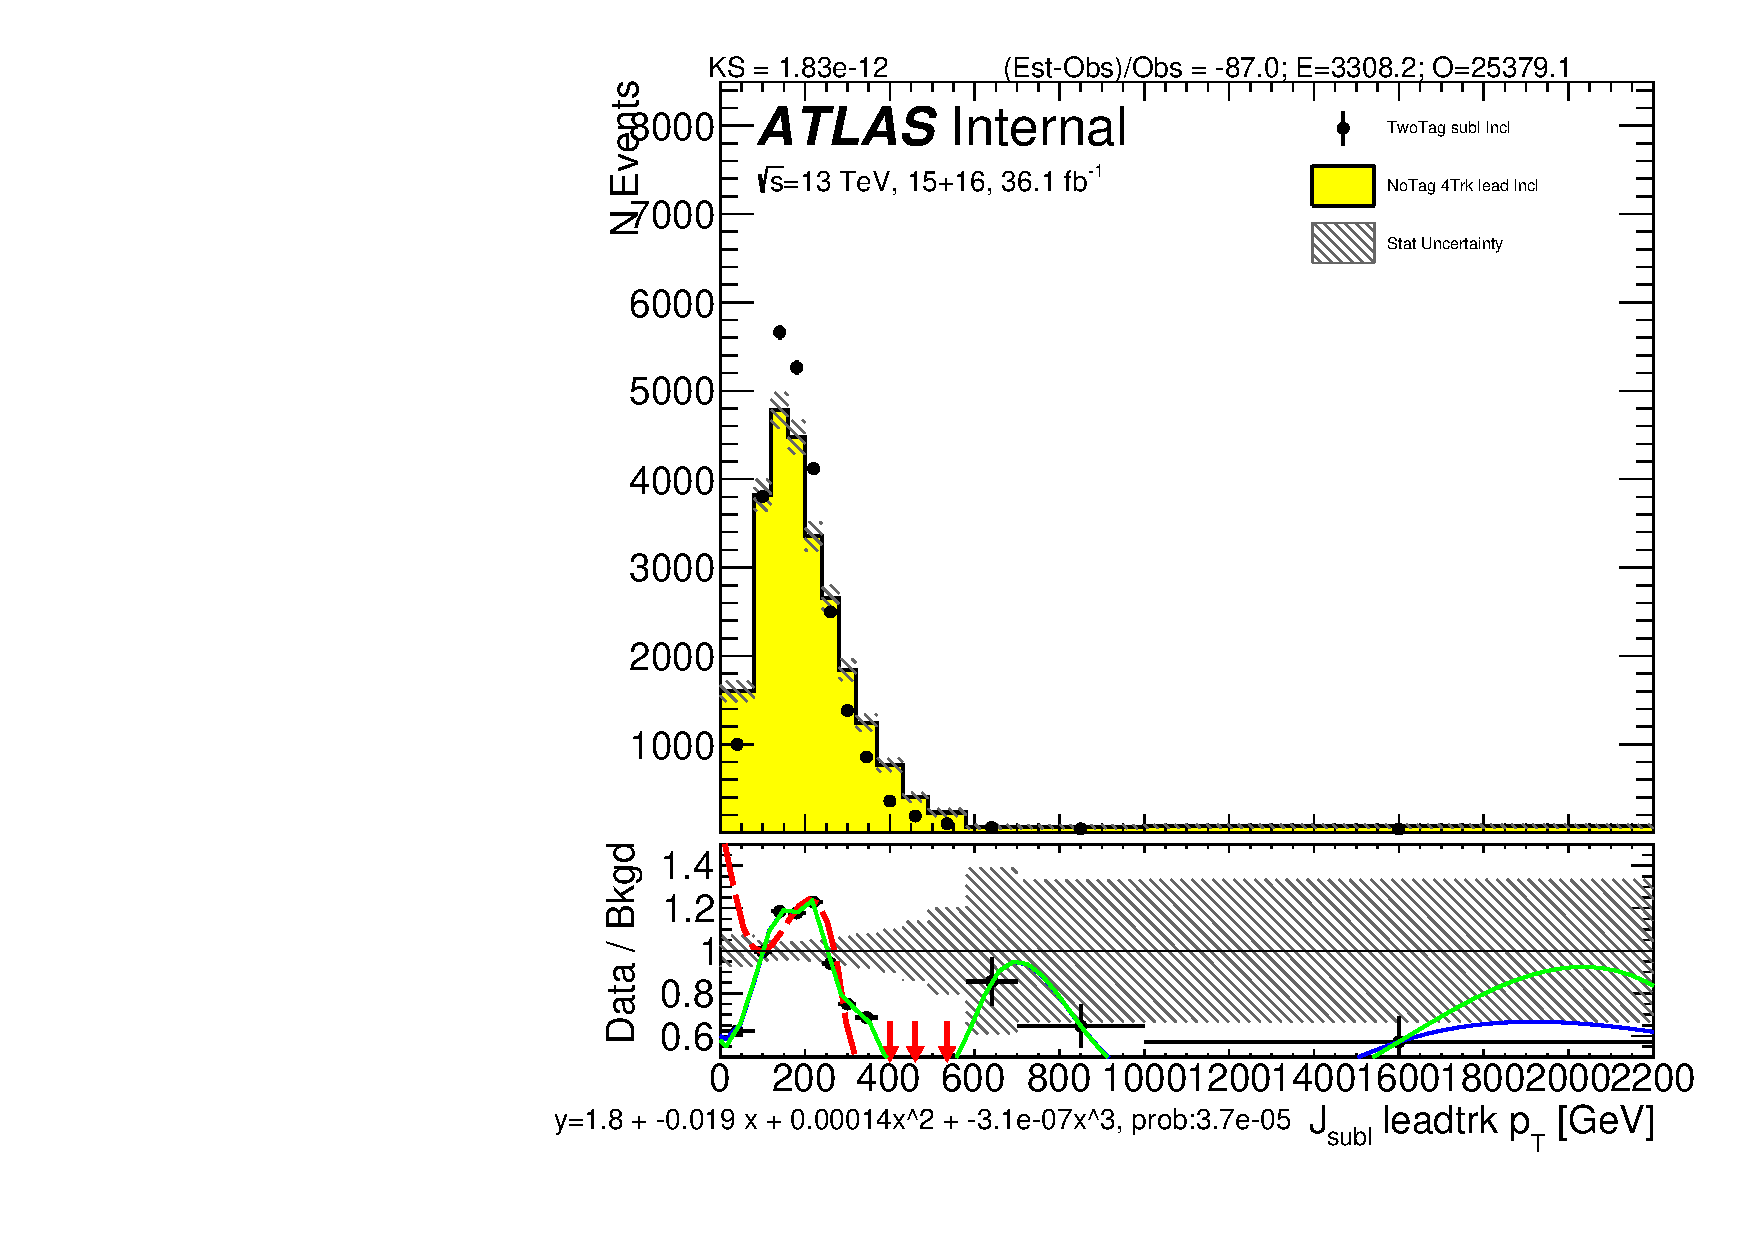
\includegraphics[width=0.25\textwidth,angle=-90]{figures/boosted/Reweight/Fits/Moriond_NoTag_4Trk_lead_Incl_sublHCand_trk0_Pt.pdf}
\includegraphics[width=0.25\textwidth,angle=-90]{figures/boosted/Reweight/Fits/Moriond_NoTag_4Trk_lead_Incl_sublHCand_trk1_Pt.pdf} \\
\includegraphics[width=0.25\textwidth,angle=-90]{figures/boosted/Reweight/Fits/Moriond_bkg_0_NoTag_4Trk_lead_Incl_sublHCand_Pt_m_1.pdf}
\includegraphics[width=0.25\textwidth,angle=-90]{figures/boosted/Reweight/Fits/Moriond_bkg_0_NoTag_4Trk_lead_Incl_sublHCand_trk0_Pt.pdf}
\includegraphics[width=0.25\textwidth,angle=-90]{figures/boosted/Reweight/Fits/Moriond_bkg_0_NoTag_4Trk_lead_Incl_sublHCand_trk1_Pt.pdf} \\
\includegraphics[width=0.25\textwidth,angle=-90]{figures/boosted/Reweight/Fits/Moriond_bkg_3_NoTag_4Trk_lead_Incl_sublHCand_Pt_m_1.pdf}
\includegraphics[width=0.25\textwidth,angle=-90]{figures/boosted/Reweight/Fits/Moriond_bkg_3_NoTag_4Trk_lead_Incl_sublHCand_trk0_Pt.pdf}
\includegraphics[width=0.25\textwidth,angle=-90]{figures/boosted/Reweight/Fits/Moriond_bkg_3_NoTag_4Trk_lead_Incl_sublHCand_trk1_Pt.pdf} \\
\includegraphics[width=0.25\textwidth,angle=-90]{figures/boosted/Reweight/Fits/Moriond_bkg_9_NoTag_4Trk_lead_Incl_sublHCand_Pt_m_1.pdf}
\includegraphics[width=0.25\textwidth,angle=-90]{figures/boosted/Reweight/Fits/Moriond_bkg_9_NoTag_4Trk_lead_Incl_sublHCand_trk0_Pt.pdf}
\includegraphics[width=0.25\textwidth,angle=-90]{figures/boosted/Reweight/Fits/Moriond_bkg_9_NoTag_4Trk_lead_Incl_sublHCand_trk1_Pt.pdf} \\
\caption{For $4b$ background estimate: the fits to the ratio of the data in the $2b$ category, of the subleading Higgs candidate $2b$-tagged events' subleading Higgs candidate distributions(black point), over the leading Higgs candidate $2b$-tagged events' subleading Higgs candidate distributions(yellow). Distributions and fits to the estimated QCD background for large-\R jet $p_{T}$ (left),  the large-\R jet's leading track jet $p_T$ (middle), and large-\R jet's subleading track jet $p_T$ (right) are shown.  Figures are before reweighting (top row), after the first iteration(second row), after the fourth iteration(third row), and after the last iteration (bottom row). The green line is the spline fit; the red line is a polynomial fit; the blue line is the spline interpolation.}
\label{fig:rw-4b-lead}
\end{center}
\end{figure*}

\begin{figure*}[htbp!]
\begin{center}
\includegraphics[width=0.25\textwidth,angle=-90]{figures/boosted/Reweight/Fits/Moriond_NoTag_4Trk_subl_Incl_leadHCand_Pt_m_1.pdf}
\includegraphics[width=0.25\textwidth,angle=-90]{figures/boosted/Reweight/Fits/Moriond_NoTag_4Trk_subl_Incl_leadHCand_trk0_Pt.pdf}
\includegraphics[width=0.25\textwidth,angle=-90]{figures/boosted/Reweight/Fits/Moriond_NoTag_4Trk_subl_Incl_leadHCand_trk1_Pt.pdf} \\
\includegraphics[width=0.25\textwidth,angle=-90]{figures/boosted/Reweight/Fits/Moriond_bkg_0_NoTag_4Trk_subl_Incl_leadHCand_Pt_m_1.pdf}
\includegraphics[width=0.25\textwidth,angle=-90]{figures/boosted/Reweight/Fits/Moriond_bkg_0_NoTag_4Trk_subl_Incl_leadHCand_trk0_Pt.pdf}
\includegraphics[width=0.25\textwidth,angle=-90]{figures/boosted/Reweight/Fits/Moriond_bkg_0_NoTag_4Trk_subl_Incl_leadHCand_trk1_Pt.pdf} \\
\includegraphics[width=0.25\textwidth,angle=-90]{figures/boosted/Reweight/Fits/Moriond_bkg_3_NoTag_4Trk_subl_Incl_leadHCand_Pt_m_1.pdf}
\includegraphics[width=0.25\textwidth,angle=-90]{figures/boosted/Reweight/Fits/Moriond_bkg_3_NoTag_4Trk_subl_Incl_leadHCand_trk0_Pt.pdf}
\includegraphics[width=0.25\textwidth,angle=-90]{figures/boosted/Reweight/Fits/Moriond_bkg_3_NoTag_4Trk_subl_Incl_leadHCand_trk1_Pt.pdf} \\
\includegraphics[width=0.25\textwidth,angle=-90]{figures/boosted/Reweight/Fits/Moriond_bkg_9_NoTag_4Trk_subl_Incl_leadHCand_Pt_m_1.pdf}
\includegraphics[width=0.25\textwidth,angle=-90]{figures/boosted/Reweight/Fits/Moriond_bkg_9_NoTag_4Trk_subl_Incl_leadHCand_trk0_Pt.pdf}
\includegraphics[width=0.25\textwidth,angle=-90]{figures/boosted/Reweight/Fits/Moriond_bkg_9_NoTag_4Trk_subl_Incl_leadHCand_trk1_Pt.pdf} \\
\caption{For $4b$ background estimate: the fits to the ratio of the data in the $2b$ category, of the leading Higgs candidate $2b$-tagged events' leading Higgs candidate distributions(black point), over the subleading Higgs candidate $2b$-tagged events' leading Higgs candidate distributions(yellow). Distributions and fits to the estimated QCD background for large-\R jet $p_{T}$ (left),  the large-\R jet's leading track jet $p_T$ (middle), and large-\R jet's subleading track jet $p_T$ (right) are shown.  Figures are before reweighting (top row), after the first iteration(second row), after the fourth iteration(third row), and after the last iteration (bottom row). The green line is the spline fit; the red line is a polynomial fit; the blue line is the spline interpolation.}
\label{fig:rw-4b-subl}
\end{center}
\end{figure*}


\paragraph{}
A comparison of the SB shapes before and after reweighting for $2bs$, $3b$ and $4b$ are shown in Figures~\ref{fig:rw-2bs-comp-sb},~\ref{fig:rw-3b-comp-sb}, and ~\ref{fig:rw-4b-comp-sb}. 
Also, a comparison of the CR shapes before and after reweighting for $2bs$, $3b$ and $4b$ can be seen in Figures~\ref{fig:rw-2bs-comp-cr},~\ref{fig:rw-3b-comp-cr}, and ~\ref{fig:rw-4b-comp-cr}. 
In almost all cases, both the reweighted/non-reweighted prediction agrees fairly well with the data, and the reweighted plots' KS scores are greater than those from non-reweighted distributions. 
%%%%%%%%%%%%%%%%%%%%%%%%%%%
\begin{figure*}[htbp!]
\begin{center}
\includegraphics[width=0.31\textwidth,angle=-90]{figures/boosted/Prereweight/Moriond_TwoTag_split_Sideband_mHH_l_1.pdf}
\includegraphics[width=0.31\textwidth,angle=-90]{figures/boosted/Sideband/b77_TwoTag_split_Sideband_mHH_l_1.pdf}\\
\includegraphics[width=0.31\textwidth,angle=-90]{figures/boosted/Prereweight/Moriond_TwoTag_split_Sideband_leadHCand_Pt_m.pdf}
\includegraphics[width=0.31\textwidth,angle=-90]{figures/boosted/Sideband/b77_TwoTag_split_Sideband_leadHCand_Pt_m.pdf}\\
\includegraphics[width=0.31\textwidth,angle=-90]{figures/boosted/Prereweight/Moriond_TwoTag_split_Sideband_leadHCand_trk0_Pt.pdf}
\includegraphics[width=0.31\textwidth,angle=-90]{figures/boosted/Sideband/b77_TwoTag_split_Sideband_leadHCand_trk0_Pt.pdf}\\
\includegraphics[width=0.31\textwidth,angle=-90]{figures/boosted/Prereweight/Moriond_TwoTag_split_Sideband_sublHCand_trk0_Pt.pdf}
\includegraphics[width=0.31\textwidth,angle=-90]{figures/boosted/Sideband/b77_TwoTag_split_Sideband_sublHCand_trk0_Pt.pdf}\\
\caption{Reweighed $2bs$ sideband region predictions comparison. Top row is the dijet Mass, second row is leading large-\R jet $p_{T}$, third row is the leading large-\R jet's leading track jet $p_T$ and the last row subleading large-\R jet's leading track jet $p_T$. On the left are the distributions before reweighting, and on the right are the distributions after reweighting.}
\label{fig:rw-2bs-comp-sb}
\end{center}
\end{figure*}


\begin{figure*}[htbp!]
\begin{center}
\includegraphics[width=0.31\textwidth,angle=-90]{figures/boosted/Prereweight/Moriond_ThreeTag_Sideband_mHH_l_1.pdf}
\includegraphics[width=0.31\textwidth,angle=-90]{figures/boosted/Sideband/b77_ThreeTag_Sideband_mHH_l_1.pdf}\\
\includegraphics[width=0.31\textwidth,angle=-90]{figures/boosted/Prereweight/Moriond_ThreeTag_Sideband_leadHCand_Pt_m.pdf}
\includegraphics[width=0.31\textwidth,angle=-90]{figures/boosted/Sideband/b77_ThreeTag_Sideband_leadHCand_Pt_m.pdf}\\
\includegraphics[width=0.31\textwidth,angle=-90]{figures/boosted/Prereweight/Moriond_ThreeTag_Sideband_leadHCand_trk0_Pt.pdf}
\includegraphics[width=0.31\textwidth,angle=-90]{figures/boosted/Sideband/b77_ThreeTag_Sideband_leadHCand_trk0_Pt.pdf}\\
\includegraphics[width=0.31\textwidth,angle=-90]{figures/boosted/Prereweight/Moriond_ThreeTag_Sideband_sublHCand_trk0_Pt.pdf}
\includegraphics[width=0.31\textwidth,angle=-90]{figures/boosted/Sideband/b77_ThreeTag_Sideband_sublHCand_trk0_Pt.pdf}\\
\caption{Reweighed $3b$ sideband region predictions comparison. Top row is the dijet Mass, second row is leading large-\R jet $p_{T}$, third row is the leading large-\R jet's leading track jet $p_T$ and the last row subleading large-\R jet's leading track jet $p_T$. On the left are the distributions before reweighting, and on the right are the distributions after reweighting.}
\label{fig:rw-3b-comp-sb}
\end{center}
\end{figure*}


\begin{figure*}[htbp!]
\begin{center}
\includegraphics[width=0.31\textwidth,angle=-90]{figures/boosted/Prereweight/Moriond_FourTag_Sideband_mHH_l_1.pdf}
\includegraphics[width=0.31\textwidth,angle=-90]{figures/boosted/Sideband/b77_FourTag_Sideband_mHH_l_1.pdf}\\
\includegraphics[width=0.31\textwidth,angle=-90]{figures/boosted/Prereweight/Moriond_FourTag_Sideband_leadHCand_Pt_m.pdf}
\includegraphics[width=0.31\textwidth,angle=-90]{figures/boosted/Sideband/b77_FourTag_Sideband_leadHCand_Pt_m.pdf}\\
\includegraphics[width=0.31\textwidth,angle=-90]{figures/boosted/Prereweight/Moriond_FourTag_Sideband_leadHCand_trk0_Pt.pdf}
\includegraphics[width=0.31\textwidth,angle=-90]{figures/boosted/Sideband/b77_FourTag_Sideband_leadHCand_trk0_Pt.pdf}\\
\includegraphics[width=0.31\textwidth,angle=-90]{figures/boosted/Prereweight/Moriond_FourTag_Sideband_sublHCand_trk0_Pt.pdf}
\includegraphics[width=0.31\textwidth,angle=-90]{figures/boosted/Sideband/b77_FourTag_Sideband_sublHCand_trk0_Pt.pdf}\\
\caption{Reweighted $4b$ sideband region predictions comparison. Top row is the dijet Mass, second row is leading large-\R jet $p_{T}$, third row is the leading large-\R jet's leading track jet $p_T$ and the last row subleading large-\R jet's leading track jet $p_T$. On the left are the distributions before reweighting, and on the right are the distributions after reweighting.}
\label{fig:rw-4b-comp-sb}
\end{center}
\end{figure*}


\begin{figure*}[htbp!]
\begin{center}
\includegraphics[width=0.31\textwidth,angle=-90]{figures/boosted/Prereweight/Moriond_TwoTag_split_Control_mHH_l_1.pdf}
\includegraphics[width=0.31\textwidth,angle=-90]{figures/boosted/Control/b77_TwoTag_split_Control_mHH_l_1.pdf}\\
\includegraphics[width=0.31\textwidth,angle=-90]{figures/boosted/Prereweight/Moriond_TwoTag_split_Control_leadHCand_Pt_m.pdf}
\includegraphics[width=0.31\textwidth,angle=-90]{figures/boosted/Control/b77_TwoTag_split_Control_leadHCand_Pt_m.pdf}\\
\includegraphics[width=0.31\textwidth,angle=-90]{figures/boosted/Prereweight/Moriond_TwoTag_split_Control_leadHCand_trk0_Pt.pdf}
\includegraphics[width=0.31\textwidth,angle=-90]{figures/boosted/Control/b77_TwoTag_split_Control_leadHCand_trk0_Pt.pdf}\\
\includegraphics[width=0.31\textwidth,angle=-90]{figures/boosted/Prereweight/Moriond_TwoTag_split_Control_sublHCand_trk0_Pt.pdf}
\includegraphics[width=0.31\textwidth,angle=-90]{figures/boosted/Control/b77_TwoTag_split_Control_sublHCand_trk0_Pt.pdf}\\
\caption{Reweighted $2bs$ control region predictions comparison. Top row is the dijet Mass, second row is leading large-\R jet $p_{T}$, third row is the leading large-\R jet's leading track jet $p_T$ and the last row subleading large-\R jet's leading track jet $p_T$. On the left are the distributions before reweighting, and on the right are the distributions after reweighting.}
\label{fig:rw-2bs-comp-cr}
\end{center}
\end{figure*}


\begin{figure*}[htbp!]
\begin{center}
\includegraphics[width=0.31\textwidth,angle=-90]{figures/boosted/Prereweight/Moriond_ThreeTag_Control_mHH_l_1.pdf}
\includegraphics[width=0.31\textwidth,angle=-90]{figures/boosted/Control/b77_ThreeTag_Control_mHH_l_1.pdf}\\
\includegraphics[width=0.31\textwidth,angle=-90]{figures/boosted/Prereweight/Moriond_ThreeTag_Control_leadHCand_Pt_m.pdf}
\includegraphics[width=0.31\textwidth,angle=-90]{figures/boosted/Control/b77_ThreeTag_Control_leadHCand_Pt_m.pdf}\\
\includegraphics[width=0.31\textwidth,angle=-90]{figures/boosted/Prereweight/Moriond_ThreeTag_Control_leadHCand_trk0_Pt.pdf}
\includegraphics[width=0.31\textwidth,angle=-90]{figures/boosted/Control/b77_ThreeTag_Control_leadHCand_trk0_Pt.pdf}\\
\includegraphics[width=0.31\textwidth,angle=-90]{figures/boosted/Prereweight/Moriond_ThreeTag_Control_sublHCand_trk0_Pt.pdf}
\includegraphics[width=0.31\textwidth,angle=-90]{figures/boosted/Control/b77_ThreeTag_Control_sublHCand_trk0_Pt.pdf}\\
\caption{Reweighted $3b$ control region predictions comparison. Top row is the dijet Mass, second row is leading large-\R jet $p_{T}$, third row is the leading large-\R jet's leading track jet $p_T$ and the last row subleading large-\R jet's leading track jet $p_T$. On the left are the distributions before reweighting, and on the right are the distributions after reweighting.}
\label{fig:rw-3b-comp-cr}
\end{center}
\end{figure*}


\begin{figure*}[htbp!]
\begin{center}
\includegraphics[width=0.31\textwidth,angle=-90]{figures/boosted/Prereweight/Moriond_FourTag_Control_mHH_l_1.pdf}
\includegraphics[width=0.31\textwidth,angle=-90]{figures/boosted/Control/b77_FourTag_Control_mHH_l_1.pdf}\\
\includegraphics[width=0.31\textwidth,angle=-90]{figures/boosted/Prereweight/Moriond_FourTag_Control_leadHCand_Pt_m.pdf}
\includegraphics[width=0.31\textwidth,angle=-90]{figures/boosted/Control/b77_FourTag_Control_leadHCand_Pt_m.pdf}\\
\includegraphics[width=0.31\textwidth,angle=-90]{figures/boosted/Prereweight/Moriond_FourTag_Control_leadHCand_trk0_Pt.pdf}
\includegraphics[width=0.31\textwidth,angle=-90]{figures/boosted/Control/b77_FourTag_Control_leadHCand_trk0_Pt.pdf}\\
\includegraphics[width=0.31\textwidth,angle=-90]{figures/boosted/Prereweight/Moriond_FourTag_Control_sublHCand_trk0_Pt.pdf}
\includegraphics[width=0.31\textwidth,angle=-90]{figures/boosted/Control/b77_FourTag_Control_sublHCand_trk0_Pt.pdf}\\
\caption{Reweighted $4b$ control region predictions comparison. Top row is the dijet Mass, second row is leading large-\R jet $p_{T}$, third row is the leading large-\R jet's leading track jet $p_T$ and the last row subleading large-\R jet's leading track jet $p_T$. On the left are the distributions before reweighting, and on the right are the distributions after reweighting.}
\label{fig:rw-4b-comp-cr}
\end{center}
\end{figure*}



\paragraph{}
More reweighting methods are tested to further validate our current reweighting method. 
The original method tries to reweight the non-Tagged Higgs candidate in the lower $b$-tagged region to be like a $b$-tagged Higgs candidate. 
This AddTag reweighting is done on three variables: large-\R jet $p_{T}$ and the two track jet $p_{T}$s, which is counted as one iteration of reweighting.

\paragraph{}
Other reweighting methods, that share similar idea with the AddTag method, where $1/2b$ samples are inclusively reweighted, have been tested:
\begin{itemize}
	\item bkgeta: AddTag reweighting, but on four variables: large-\R jet $p_{T}$, the two track jet $p_{T}$s, and large-\R jet $\eta$.
	\item bkgdr: AddTag reweighting, but on four variables: large-\R jet $p_{T}$, the two track jet $p_{T}$s, and two track jet $\Delta R$.
	\item bkgtrk: AddTag reweighting, but on two variables: only the two track jet $p_{T}$s.
	\item bkgsb: AddTag reweighting, using the same three variables but instead of reweighting the $1b$ non-tagged Higgs candidate to be like the $1b$ tagged Higgs candidate, reweight $1b$ non-tagged Higgs candidate's distributions to be like the $2bs$ Higgs candidate in the sideband. Similarly, for $3b$, reweight $2b$ non-tagged Higgs candidate's distributions to be like the $3b$ Higgs candidate in the sideband, and for $4b$, reweight $2b$ non-tagged Higgs candidate's distributions to be like the $4b$ Higgs candidate in the sideband.
\end{itemize}

\paragraph{}
Also, reweighting the $1b$ Sideband directly to be like $2bs$ Sideband, and propagate the weight to control and signal regions, as the method used for previous analysis, has been tested:
\begin{itemize}
	\item leadtrk: on three variables: leading Higgs candidate large-\R jet $p_{T}$, the two lead-track jet $p_{T}$s.
	\item subltrk: on three variables: leading Higgs candidate large-\R jet $p_{T}$, the two subllead-track jet $p_{T}$s.
	\item alltrk: on five variables: leading Higgs candidate large-\R jet $p_{T}$, the two lead-track jet $p_{T}$s, and the two subllead-track jet $p_{T}$s.
\end{itemize}

\paragraph{}
For \mtwoJ, the dijet mass distribution, the distribution comparisons are shown in Figure ~\ref{fig:app-rw-comp}. Signal regions are blinded, and the data distribution is replaced with the non-reweighted background estimate. 
For track jet \pt distributions, the comparisons are shown in Figure ~\ref{fig:app-rw-comp-2bs-trkjet}, ~\ref{fig:app-rw-comp-3b-trkjet}, ~\ref{fig:app-rw-comp-4b-trkjet}. 
In most cases, the $\chi^2$ per degree of freedom is improved for the background estimations, and very similar distributions in signal region is observed. Hence no extra systematics is assigned for the reweighting method.

\begin{figure*}[htbp!]
\begin{center}
\includegraphics[width=0.3\textwidth,angle=-90]{figures/boosted/AppendixReweight/Compare/Data_TwoTag_split_Sideband_directcompare_mHH_l_1.pdf}
\includegraphics[width=0.3\textwidth,angle=-90]{figures/boosted/AppendixReweight/Compare/Data_ThreeTag_Sideband_directcompare_mHH_l_1.pdf}
\includegraphics[width=0.3\textwidth,angle=-90]{figures/boosted/AppendixReweight/Compare/Data_FourTag_Sideband_directcompare_mHH_l_1.pdf}\\
\includegraphics[width=0.3\textwidth,angle=-90]{figures/boosted/AppendixReweight/Compare/Data_TwoTag_split_Control_directcompare_mHH_l_1.pdf}
\includegraphics[width=0.3\textwidth,angle=-90]{figures/boosted/AppendixReweight/Compare/Data_ThreeTag_Control_directcompare_mHH_l_1.pdf}
\includegraphics[width=0.3\textwidth,angle=-90]{figures/boosted/AppendixReweight/Compare/Data_FourTag_Control_directcompare_mHH_l_1.pdf}\\
\includegraphics[width=0.3\textwidth,angle=-90]{figures/boosted/AppendixReweight/Compare/Data_TwoTag_split_Signal_directcompare_mHH_l_1.pdf}
\includegraphics[width=0.3\textwidth,angle=-90]{figures/boosted/AppendixReweight/Compare/Data_ThreeTag_Signal_directcompare_mHH_l_1.pdf}
\includegraphics[width=0.3\textwidth,angle=-90]{figures/boosted/AppendixReweight/Compare/Data_FourTag_Signal_directcompare_mHH_l_1.pdf}
\caption{Reweighted $2bs$ (left column), $3b$ (middle column), and $4b$ (right column) sideband (top row), control (middle row) and signal (bottom row) region predictions comparison, for MJJ. The Signal region is blinded, and the data distribution is replaced with the non-reweighted background predictions.}
\label{fig:app-rw-comp}
\end{center}
\end{figure*}

\begin{figure*}[htbp!]
\begin{center}
\includegraphics[width=0.21\textwidth,angle=-90]{figures/boosted/AppendixReweight/Compare/Data_TwoTag_split_Sideband_directcompare_leadHCand_trk0_Pt_1.pdf}
\includegraphics[width=0.21\textwidth,angle=-90]{figures/boosted/AppendixReweight/Compare/Data_TwoTag_split_Sideband_directcompare_leadHCand_trk1_Pt_1.pdf}
\includegraphics[width=0.21\textwidth,angle=-90]{figures/boosted/AppendixReweight/Compare/Data_TwoTag_split_Sideband_directcompare_sublHCand_trk0_Pt_1.pdf}
\includegraphics[width=0.21\textwidth,angle=-90]{figures/boosted/AppendixReweight/Compare/Data_TwoTag_split_Sideband_directcompare_sublHCand_trk1_Pt_1.pdf}\\
\includegraphics[width=0.21\textwidth,angle=-90]{figures/boosted/AppendixReweight/Compare/Data_TwoTag_split_Control_directcompare_leadHCand_trk0_Pt_1.pdf}
\includegraphics[width=0.21\textwidth,angle=-90]{figures/boosted/AppendixReweight/Compare/Data_TwoTag_split_Control_directcompare_leadHCand_trk1_Pt_1.pdf}
\includegraphics[width=0.21\textwidth,angle=-90]{figures/boosted/AppendixReweight/Compare/Data_TwoTag_split_Control_directcompare_sublHCand_trk0_Pt_1.pdf}
\includegraphics[width=0.21\textwidth,angle=-90]{figures/boosted/AppendixReweight/Compare/Data_TwoTag_split_Control_directcompare_sublHCand_trk1_Pt_1.pdf}\\
\includegraphics[width=0.21\textwidth,angle=-90]{figures/boosted/AppendixReweight/Compare/Data_TwoTag_split_Signal_directcompare_leadHCand_trk0_Pt_1.pdf}
\includegraphics[width=0.21\textwidth,angle=-90]{figures/boosted/AppendixReweight/Compare/Data_TwoTag_split_Signal_directcompare_leadHCand_trk1_Pt_1.pdf}
\includegraphics[width=0.21\textwidth,angle=-90]{figures/boosted/AppendixReweight/Compare/Data_TwoTag_split_Signal_directcompare_sublHCand_trk0_Pt_1.pdf}
\includegraphics[width=0.21\textwidth,angle=-90]{figures/boosted/AppendixReweight/Compare/Data_TwoTag_split_Signal_directcompare_sublHCand_trk1_Pt_1.pdf}\\
\caption{Reweighted $2bs$ sideband (top row), control (middle row) and signal (bottom row) region predictions comparison, for leading Higgs Candidate leading track jet \pt~ (first column),  leading Higgs Candidate subleading track jet \pt~ (second column), subleading Higgs Candidate leading track jet \pt~ (third column), subleading Higgs Candidate subleading track jet \pt~ (fourth column). The signal region is blinded, where the distribution is replaced with the non-reweighted predictions.}
\label{fig:app-rw-comp-2bs-trkjet}
\end{center}
\end{figure*}

\begin{figure*}[htbp!]
\begin{center}
\includegraphics[width=0.21\textwidth,angle=-90]{figures/boosted/AppendixReweight/Compare/Data_ThreeTag_Sideband_directcompare_leadHCand_trk0_Pt_1.pdf}
\includegraphics[width=0.21\textwidth,angle=-90]{figures/boosted/AppendixReweight/Compare/Data_ThreeTag_Sideband_directcompare_leadHCand_trk1_Pt_1.pdf}
\includegraphics[width=0.21\textwidth,angle=-90]{figures/boosted/AppendixReweight/Compare/Data_ThreeTag_Sideband_directcompare_sublHCand_trk0_Pt_1.pdf}
\includegraphics[width=0.21\textwidth,angle=-90]{figures/boosted/AppendixReweight/Compare/Data_ThreeTag_Sideband_directcompare_sublHCand_trk1_Pt_1.pdf}\\
\includegraphics[width=0.21\textwidth,angle=-90]{figures/boosted/AppendixReweight/Compare/Data_ThreeTag_Control_directcompare_leadHCand_trk0_Pt_1.pdf}
\includegraphics[width=0.21\textwidth,angle=-90]{figures/boosted/AppendixReweight/Compare/Data_ThreeTag_Control_directcompare_leadHCand_trk1_Pt_1.pdf}
\includegraphics[width=0.21\textwidth,angle=-90]{figures/boosted/AppendixReweight/Compare/Data_ThreeTag_Control_directcompare_sublHCand_trk0_Pt_1.pdf}
\includegraphics[width=0.21\textwidth,angle=-90]{figures/boosted/AppendixReweight/Compare/Data_ThreeTag_Control_directcompare_sublHCand_trk1_Pt_1.pdf}\\
\includegraphics[width=0.21\textwidth,angle=-90]{figures/boosted/AppendixReweight/Compare/Data_ThreeTag_Signal_directcompare_leadHCand_trk0_Pt_1.pdf}
\includegraphics[width=0.21\textwidth,angle=-90]{figures/boosted/AppendixReweight/Compare/Data_ThreeTag_Signal_directcompare_leadHCand_trk1_Pt_1.pdf}
\includegraphics[width=0.21\textwidth,angle=-90]{figures/boosted/AppendixReweight/Compare/Data_ThreeTag_Signal_directcompare_sublHCand_trk0_Pt_1.pdf}
\includegraphics[width=0.21\textwidth,angle=-90]{figures/boosted/AppendixReweight/Compare/Data_ThreeTag_Signal_directcompare_sublHCand_trk1_Pt_1.pdf}\\
\caption{Reweighted $3b$ sideband (top row), control (middle row) and signal (bottom row) predictions comparison, for leading Higgs Candidate leading track jet \pt~ (first column),  leading Higgs Candidate subleading track jet \pt~ (second column), subleading Higgs Candidate leading track jet \pt (third column), subleading Higgs Candidate subleading track jet \pt~ (fourth column). The signal region is blinded, where the distribution is replaced with the non-reweighted predictions.}
\label{fig:app-rw-comp-3b-trkjet}
\end{center}
\end{figure*}

\begin{figure*}[htbp!]
\begin{center}
\includegraphics[width=0.21\textwidth,angle=-90]{figures/boosted/AppendixReweight/Compare/Data_FourTag_Sideband_directcompare_leadHCand_trk0_Pt_1.pdf}
\includegraphics[width=0.21\textwidth,angle=-90]{figures/boosted/AppendixReweight/Compare/Data_FourTag_Sideband_directcompare_leadHCand_trk1_Pt_1.pdf}
\includegraphics[width=0.21\textwidth,angle=-90]{figures/boosted/AppendixReweight/Compare/Data_FourTag_Sideband_directcompare_sublHCand_trk0_Pt_1.pdf}
\includegraphics[width=0.21\textwidth,angle=-90]{figures/boosted/AppendixReweight/Compare/Data_FourTag_Sideband_directcompare_sublHCand_trk1_Pt_1.pdf}\\
\includegraphics[width=0.21\textwidth,angle=-90]{figures/boosted/AppendixReweight/Compare/Data_FourTag_Control_directcompare_leadHCand_trk0_Pt_1.pdf}
\includegraphics[width=0.21\textwidth,angle=-90]{figures/boosted/AppendixReweight/Compare/Data_FourTag_Control_directcompare_leadHCand_trk1_Pt_1.pdf}
\includegraphics[width=0.21\textwidth,angle=-90]{figures/boosted/AppendixReweight/Compare/Data_FourTag_Control_directcompare_sublHCand_trk0_Pt_1.pdf}
\includegraphics[width=0.21\textwidth,angle=-90]{figures/boosted/AppendixReweight/Compare/Data_FourTag_Control_directcompare_sublHCand_trk1_Pt_1.pdf}\\
\includegraphics[width=0.21\textwidth,angle=-90]{figures/boosted/AppendixReweight/Compare/Data_FourTag_Signal_directcompare_leadHCand_trk0_Pt_1.pdf}
\includegraphics[width=0.21\textwidth,angle=-90]{figures/boosted/AppendixReweight/Compare/Data_FourTag_Signal_directcompare_leadHCand_trk1_Pt_1.pdf}
\includegraphics[width=0.21\textwidth,angle=-90]{figures/boosted/AppendixReweight/Compare/Data_FourTag_Signal_directcompare_sublHCand_trk0_Pt_1.pdf}
\includegraphics[width=0.21\textwidth,angle=-90]{figures/boosted/AppendixReweight/Compare/Data_FourTag_Signal_directcompare_sublHCand_trk1_Pt_1.pdf}\\
\caption{Reweighted $4b$ sideband (top row), control (middle row) and signal (bottom row) region predictions comparison, for leading Higgs Candidate leading track jet \pt~ (first column),  leading Higgs Candidate subleading track jet \pt~ (second column), subleading Higgs Candidate leading track jet \pt~ (third column), subleading Higgs Candidate subleading track jet \pt (fourth column). The signal region is blinded, where the distribution is replaced with the non-reweighted predictions.}
\label{fig:app-rw-comp-4b-trkjet}
\end{center}
\end{figure*}


\paragraph{}
The reweighting method can be further validated using Dijet MC. 
Due to the limited statistics, only $2bs$ dijet MC has enough event for testing. The weights derived in data are applied in the MC $1b$ using the AddTag method, and compared with the $1b$ un-reweighted distribution and the $2bs$ distribution. 
The inclusive region (sideband + control + signal) track jet \pt~ distributions are shown in Figure ~\ref{fig:app-rw-comp-dijet-2bs-trkjet}. As can be seen, reweighting helps to model different $b$ tagging sculpting effect. 
The \mtwoJ~ distributions can be seen in Figure ~\ref{fig:app-rw-comp-dijet-2bs}. 
Reweighting differs from the non-reweighted distribution only by a small amount, yet improves the overall $\chi^2$ per degree of freedom.

%%%%%%%%%%%%%%%%%%%%%%%%%%%
\begin{figure*}[htbp!]
\begin{center}
\includegraphics[width=0.48\textwidth,angle=-90]{figures/boosted/AppendixReweight/Compare/Dijet_Incl_directcompare_leadHCand_trk0_Pt_1.pdf}
\includegraphics[width=0.48\textwidth,angle=-90]{figures/boosted/AppendixReweight/Compare/Dijet_Incl_directcompare_leadHCand_trk1_Pt_1.pdf}\\
\includegraphics[width=0.48\textwidth,angle=-90]{figures/boosted/AppendixReweight/Compare/Dijet_Incl_directcompare_sublHCand_trk0_Pt_1.pdf}
\includegraphics[width=0.48\textwidth,angle=-90]{figures/boosted/AppendixReweight/Compare/Dijet_Incl_directcompare_sublHCand_trk1_Pt_1.pdf}\\
\caption{Reweighted $2bs$ inclusive region predictions comparison in dijet MC, for leading Higgs Candidate leading track jet \pt (top left),  leading Higgs Candidate subleading track jet \pt (top right), subleading Higgs Candidate leading track jet \pt (bottom left), subleading Higgs Candidate subleading track jet \pt (bottom right). $1b$ and reweighted $1b$ distributions are normalized to $2bs$.}
\label{fig:app-rw-comp-dijet-2bs-trkjet}
\end{center}
\end{figure*}

\begin{figure*}[htbp!]
\begin{center}
\includegraphics[width=0.4\textwidth,angle=-90]{figures/boosted/AppendixReweight/Compare/Dijet_Sideband_directcompare_mHH_l_1.pdf}\\
\includegraphics[width=0.4\textwidth,angle=-90]{figures/boosted/AppendixReweight/Compare/Dijet_Control_directcompare_mHH_l_1.pdf}\\
\includegraphics[width=0.4\textwidth,angle=-90]{figures/boosted/AppendixReweight/Compare/Dijet_Signal_directcompare_mHH_l_1.pdf}
\caption{Reweighted $2bs$ sideband (top) / control (middle) / signal (bottom) region predictions comparison, for MJJ. The signal region is not blinded, since it is dijet MC distribution. $1b$ and reweighted $1b$ distributions are normalized to $2bs$.}
\label{fig:app-rw-comp-dijet-2bs}
\end{center}
\end{figure*}

\clearpage